\documentclass[twoside]{book}

% Packages required by doxygen
\usepackage{fixltx2e}
\usepackage{calc}
\usepackage{doxygen}
\usepackage[export]{adjustbox} % also loads graphicx
\usepackage{graphicx}
\usepackage[utf8]{inputenc}
\usepackage{makeidx}
\usepackage{multicol}
\usepackage{multirow}
\PassOptionsToPackage{warn}{textcomp}
\usepackage{textcomp}
\usepackage[nointegrals]{wasysym}
\usepackage[table]{xcolor}

% Font selection
\usepackage[T1]{fontenc}
\usepackage[scaled=.90]{helvet}
\usepackage{courier}
\usepackage{amssymb}
\usepackage{sectsty}
\renewcommand{\familydefault}{\sfdefault}
\allsectionsfont{%
  \fontseries{bc}\selectfont%
  \color{darkgray}%
}
\renewcommand{\DoxyLabelFont}{%
  \fontseries{bc}\selectfont%
  \color{darkgray}%
}
\newcommand{\+}{\discretionary{\mbox{\scriptsize$\hookleftarrow$}}{}{}}

% Page & text layout
\usepackage{geometry}
\geometry{%
  a4paper,%
  top=2.5cm,%
  bottom=2.5cm,%
  left=2.5cm,%
  right=2.5cm%
}
\tolerance=750
\hfuzz=15pt
\hbadness=750
\setlength{\emergencystretch}{15pt}
\setlength{\parindent}{0cm}
\setlength{\parskip}{3ex plus 2ex minus 2ex}
\makeatletter
\renewcommand{\paragraph}{%
  \@startsection{paragraph}{4}{0ex}{-1.0ex}{1.0ex}{%
    \normalfont\normalsize\bfseries\SS@parafont%
  }%
}
\renewcommand{\subparagraph}{%
  \@startsection{subparagraph}{5}{0ex}{-1.0ex}{1.0ex}{%
    \normalfont\normalsize\bfseries\SS@subparafont%
  }%
}
\makeatother

% Headers & footers
\usepackage{fancyhdr}
\pagestyle{fancyplain}
\fancyhead[LE]{\fancyplain{}{\bfseries\thepage}}
\fancyhead[CE]{\fancyplain{}{}}
\fancyhead[RE]{\fancyplain{}{\bfseries\leftmark}}
\fancyhead[LO]{\fancyplain{}{\bfseries\rightmark}}
\fancyhead[CO]{\fancyplain{}{}}
\fancyhead[RO]{\fancyplain{}{\bfseries\thepage}}
\fancyfoot[LE]{\fancyplain{}{}}
\fancyfoot[CE]{\fancyplain{}{}}
\fancyfoot[RE]{\fancyplain{}{\bfseries\scriptsize Generated by Doxygen }}
\fancyfoot[LO]{\fancyplain{}{\bfseries\scriptsize Generated by Doxygen }}
\fancyfoot[CO]{\fancyplain{}{}}
\fancyfoot[RO]{\fancyplain{}{}}
\renewcommand{\footrulewidth}{0.4pt}
\renewcommand{\chaptermark}[1]{%
  \markboth{#1}{}%
}
\renewcommand{\sectionmark}[1]{%
  \markright{\thesection\ #1}%
}

% Indices & bibliography
\usepackage{natbib}
\usepackage[titles]{tocloft}
\setcounter{tocdepth}{3}
\setcounter{secnumdepth}{5}
\makeindex

% Hyperlinks (required, but should be loaded last)
\usepackage{ifpdf}
\ifpdf
  \usepackage[pdftex,pagebackref=true]{hyperref}
\else
  \usepackage[ps2pdf,pagebackref=true]{hyperref}
\fi
\hypersetup{%
  colorlinks=true,%
  linkcolor=blue,%
  citecolor=blue,%
  unicode%
}

% Custom commands
\newcommand{\clearemptydoublepage}{%
  \newpage{\pagestyle{empty}\cleardoublepage}%
}

\usepackage{caption}
\captionsetup{labelsep=space,justification=centering,font={bf},singlelinecheck=off,skip=4pt,position=top}

%===== C O N T E N T S =====

\begin{document}

% Titlepage & ToC
\hypersetup{pageanchor=false,
             bookmarksnumbered=true,
             pdfencoding=unicode
            }
\pagenumbering{roman}
\begin{titlepage}
\vspace*{7cm}
\begin{center}%
{\Large Bio\+C\+A\+Se Monitor \\[1ex]\large 2.\+1 }\\
\vspace*{1cm}
{\large Generated by Doxygen 1.8.11}\\
\end{center}
\end{titlepage}
\clearemptydoublepage
\tableofcontents
\clearemptydoublepage
\pagenumbering{arabic}
\hypersetup{pageanchor=true}

%--- Begin generated contents ---
\chapter{Bio\+C\+A\+Se Monitor 2.1}
\label{index}\hypertarget{index}{}\begin{DoxyCopyright}{Copyright}
(C) 2013-\/2018 www.\+naturkundemuseum.\+berlin
\end{DoxyCopyright}
\begin{DoxyAuthor}{Author}
\href{mailto:thomas.pfuhl@mfn-berlin.de}{\tt thomas.\+pfuhl@mfn-\/berlin.\+de}
\end{DoxyAuthor}
based on Version 1.\+4 written by \href{mailto:falko.gloeckler@mfn-berlin.de}{\tt falko.\+gloeckler@mfn-\/berlin.\+de}

This program is free software\+: you can redistribute it and/or modify it under the terms of the G\+NU General Public License as published by the Free Software Foundation, either version 3 of the License, or (at your option) any later version.

This program is distributed in the hope that it will be useful, but W\+I\+T\+H\+O\+UT A\+NY W\+A\+R\+R\+A\+N\+TY; without even the implied warranty of M\+E\+R\+C\+H\+A\+N\+T\+A\+B\+I\+L\+I\+TY or F\+I\+T\+N\+E\+SS F\+OR A P\+A\+R\+T\+I\+C\+U\+L\+AR P\+U\+R\+P\+O\+SE. See the G\+NU General Public License for more details.

You should have received a copy of the G\+NU General Public License along with this program. If not, see \href{http://www.gnu.org/licenses/}{\tt http\+://www.\+gnu.\+org/licenses/}.





\section*{Purpose}

The Bio\+C\+A\+Se Monitor Service (B\+MS) is a tool for coordinators of networks of biodiversity databases that are based on the Bio\+C\+A\+Se Provider Software (B\+PS).

The backend part of the tool allows registration of Bio\+C\+A\+Se providers and their data sources in a user-\/friendly UI.

In the frontend, all relevant information are displayed in an aggregated view, e.\+g.
\begin{DoxyItemize}
\item provider name (linking to the access point U\+RL),
\item list of data sources, total number of records and of unique values per concept (i.\+e. number of units, number of multimedia objects),
\item link to the consistency checker tool
\item link to archives
\item other useful links.
\end{DoxyItemize}

In the EU funded project Open\+Up! the Bio\+C\+A\+Se Monitor Service is used to monitor the progress of the provision of multimedia objects to Europeana.

Furthermore, it is a useful tool for the coordinators of the content-\/providing work packages as a quality check of the mapping of the associated metadata in the A\+B\+CD or A\+B\+C\+D\+E\+FG schema and its required compliance with the Europeana Sematic Elements (E\+SE), the Europeana standard. The tool has been developed in close collaboration between the Open\+Up! team (Work Package 4 \& 7) and the G\+B\+I\+F-\/D team at the Museum für Naturkunde Berlin, Germany.

The version series 2.\+x code has been completely rewritten, and relies on a sqlite3 database.

A more detailed description has been published in the \href{https://www.ncbi.nlm.nih.gov/pmc/articles/PMC3964725/}{\tt Biodiversity Data Journal}

\section*{\hyperlink{namespace_webservices}{Webservices}}

As a complement of the G\+UI, the software offers \hyperlink{namespace_webservices}{Webservices}. The entry point is \href{/services/}{\tt services/}





\section*{Installation}

\subsection*{Requirements}


\begin{DoxyItemize}
\item Webserver, e.\+g. apache2
\item Database engine, e.\+g. sqlite3
\item P\+DO
\item P\+HP 5.\+6
\item php5-\/curl, php5-\/sqlite, php5-\/xsl
\end{DoxyItemize}

\subsection*{Installation steps}


\begin{DoxyEnumerate}
\item copy everything to a webfolder
\item edit configuration file {\ttfamily config/config.\+php}
\item set files permissions
\begin{DoxyItemize}
\item all files must be readable by webuser
\item DB file {\ttfamily provider.\+sqlite} must be writable by webuser
\item Cache folder {\ttfamily data\+\_\+cache} must be writable by webuser
\end{DoxyItemize}
\item create and populate database
\begin{DoxyItemize}
\item run statements defined in {\ttfamily install/sampledata.\+sql}
\end{DoxyItemize}
\end{DoxyEnumerate}

The following shell script {\ttfamily install/install.\+sh} does the job for an installation on linux. You might be required to have sudoer\textquotesingle{}s rights\+: \begin{DoxyVerb}#!/bin/bash
# please edit these settings
DBDIR=/my/db/folder/ 
WEBDIR=/var/www/bms 
WEBUSER=www-data  
# running the commands
mkdir $DBDIR  
mkdir $WEBDIR  
cd $WEBDIR  
chgrp -R $WEBUSER .  
chmod -R g+w $DBDIR   
mkdir data_cache  
chmod g+w data_cache 
cd config
ln -s config.sample.php config.php
mv sampledata.sql $DBDIR  
sqlite3 $DBDIR/provider.sqlite < $DBDIR/sampledata.sql
chgrp $WEBUSER $DBDIR/provider.sqlite
\end{DoxyVerb}


\subsection*{Backend}

In the navigation bar, log in. Default administrator account\+: {\ttfamily username=admin}, {\ttfamily password=admin}.

\subsection*{A\+PI Documentation}

Point your browser to {\ttfamily info/doc/api/html/index.\+html}

\subsection*{Typical Administrator\textquotesingle{}s Workflow}


\begin{DoxyEnumerate}
\item Login
\begin{DoxyItemize}
\item Login via the navigation bar
\item type in your credentials and validate
\item select a provider in the dropdown list
\end{DoxyItemize}
\item Main Metadata
\begin{DoxyItemize}
\item edit the provider\textquotesingle{}s Main Metadata
\end{DoxyItemize}
\item Count Concepts
\begin{DoxyItemize}
\item example\+: {\ttfamily /\+Data\+Set/\+Units/\+Unit/\+Multi\+Media\+Objects/\+Multi\+Media\+Object/\+File\+U\+RI}
\item modify a concept\+: autocompletion from all concepts defined in A\+B\+C\+D2
\item move a concept up and down, using the handle
\item save the current concept count
\item delete the current concept count
\item add a new concept count
\end{DoxyItemize}
\item Data Source Access Points (D\+S\+As)
\begin{DoxyItemize}
\item Data Sources
\begin{DoxyItemize}
\item Data Sources are presented in tabs\+: a tab for each data set, one data source visible
\item operations\+: {\ttfamily add}, {\ttfamily delete}, {\ttfamily save}
\item edit required fields
\begin{DoxyItemize}
\item status\+: active/inactive
\end{DoxyItemize}
\item data-\/source\+: select select a specific Data Source in the dropdown list
\item title\+: type a human readable full title
\item data-\/set\+: select a specific Data Set in the dropdown list
\item landing-\/page\+: select type of landingpge\+:
\begin{DoxyItemize}
\item automatically generated\+: this is the default landingpage, based on a scan request for the concept {\ttfamily /\+Data\+Sets/\+Data\+Set/\+Units/\+Unit/\+Multi\+Media\+Objects/\+Multi\+Media\+Object/\+File\+U\+RI}.
\item user-\/defined U\+RL\+: enter an U\+RL
\end{DoxyItemize}
\item for advanced users only\+:
\begin{DoxyItemize}
\item filter\+: define a complex filter
\item Beware ! The filter is applied {\bfseries as is} (not validated) to the request sent to the pywrapper
\end{DoxyItemize}
\end{DoxyItemize}
\item Archives
\begin{DoxyItemize}
\item add an arbitrary list of archives
\item an archive is a U\+RL pointing to a downloadable file
\item one archive must be marked as \char`\"{}latest\char`\"{}
\end{DoxyItemize}
\item Useful Links
\begin{DoxyItemize}
\item add an arbitrary list of links
\item a link is a U\+RL pointing to a downloadable file and should be one of the following types\+:
\begin{DoxyItemize}
\item Bio\+C\+A\+Se Query Tool
\item G\+B\+IF
\item Europaeana
\item Deutsche Digitale Bibliothek
\item Geo\+C\+A\+Se
\item Bi\+N\+Hum
\item Pangaea
\item G\+F\+Bio
\end{DoxyItemize}
\item example\+: {\ttfamily \href{http://www.gbif.org/dataset/71f03224-f762-11e1-a439-00145eb45e9a}{\tt http\+://www.\+gbif.\+org/dataset/71f03224-\/f762-\/11e1-\/a439-\/00145eb45e9a}} (G\+B\+IF)
\end{DoxyItemize}
\end{DoxyItemize}
\item Logout
\begin{DoxyItemize}
\item log out via the navigation bar
\end{DoxyItemize}
\end{DoxyEnumerate}





\section*{Issues}

The B\+MS has been tested on Firefox and Chrome. It has been reported that Opera and IE do not display the data. 
\chapter{B\+MS Consistency Check -\/ Todo List}
\label{md_util_schemamappings_data_todo}
\hypertarget{md_util_schemamappings_data_todo}{}
\subsection*{Dw\+Core}


\begin{DoxyItemize}
\item use recommended version
\item take complete xpath
\item reference\+: \href{http://rs.tdwg.org/dwc/terms/Occurrence}{\tt http\+://rs.\+tdwg.\+org/dwc/terms/\+Occurrence}
\item make decision which A\+B\+CD xpath to select\+:

\{Data\+Sets/\+Data\+Set/\+Units/\+Unit/\+Record\+U\+RI {\bfseries or} Datasets/\+Dataset/\+Units/\+Unit/\+Unit\+References/\+Unit\+References {\bfseries or} Datasets/\+Dataset/\+Units/\+Unit/\+Source\+Reference {\bfseries or} Datasets/\+Dataset/\+Units/\+Unit/\+Identifications/\+Identification/\+References/\+Reference {\bfseries or} Datasets/\+Dataset/\+Units/\+Unit/\+Specimen\+Unit/\+Nomenclatural\+Type\+Designations/\+Nomenclatural\+Type\+Designation/\+Nomenclatural\+Reference {\bfseries or} Measurement\+Or\+Fact/\+Measurement\+Or\+Fact\+Atomised/\+Measurement\+Or\+Fact\+Reference\}
\item how to process things like\+:

associated\+Sequences Data\+Sets/\+Data\+Set/\+Units/\+Unit/\+Sequences/\+Sequence/\+I\+D-\/in-\/\+Database + constant previous\+Identifications Data\+Sets/\+Data\+Set/\+Units/\+Unit/\+Identifications/\+Identification with Preferred\+Flag = false continent Data\+Sets/\+Data\+Set/\+Units/\+Unit/\+Gathering/\+Named\+Areas/\+Named\+Area/\+Area\+Name with Named\+Areas/\+Named\+Area/\+Area\+Class= Continent 
\end{DoxyItemize}
\chapter{Todo List}
\label{todo}
\hypertarget{todo}{}

\begin{DoxyRefList}
\item[\label{todo__todo000008}%
\hypertarget{todo__todo000008}{}%
Global \hyperlink{backend_8js_a771a32402016a259aee9ff74cd879048}{add\+Count} ()]\+: attach count concepts to each D\+SA, since d\+D\+S\+As may have distinct schemas  
\item[\label{todo__todo000002}%
\hypertarget{todo__todo000002}{}%
File \hyperlink{check_for_errors_8php}{check\+For\+Errors.php} ]classify rules depending on the weight 
\item[\label{todo__todo000003}%
\hypertarget{todo__todo000003}{}%
File \hyperlink{check_rules_8php}{check\+Rules.php} ]C\+U\+RL request can be time consuming 
\item[\label{todo__todo000005}%
\hypertarget{todo__todo000005}{}%
Global \hyperlink{namespace_consistency_a6de4812dd264c558f2dadf3ae20b1da2}{Consistency\+:\+:\$concept\+\_\+xpath} ]compute element xpath with correct prefix for given schema  
\item[\label{todo__todo000006}%
\hypertarget{todo__todo000006}{}%
Global \hyperlink{namespace_consistency_aa98f8a888d842fcaefeca3407c10435c}{Consistency\+:\+:get\+Schema\+Mappings} (\$mapping)]add parameter dataset, and restrict result to supported Schemas  
\item[\label{todo__todo000001}%
\hypertarget{todo__todo000001}{}%
File \hyperlink{get_all_count_concepts_8php}{get\+All\+Count\+Concepts.php} ]filter through given schema 

move it to services 
\item[\label{todo__todo000004}%
\hypertarget{todo__todo000004}{}%
File \hyperlink{get_example_values_8php}{get\+Example\+Values.php} ]compute element xpath with correct prefix for given schema 
\item[\label{todo__todo000007}%
\hypertarget{todo__todo000007}{}%
File \hyperlink{consistency_2index_8php}{index.php} ]call webservice via A\+J\+AX\+: \char`\"{}../services/providers/index.\+php\char`\"{}  
\item[\label{todo__todo000010}%
\hypertarget{todo__todo000010}{}%
Global \hyperlink{consistency_8js_a0cd14e63b9113fcee3fa0e999aa1ada9}{is\+Valid\+Citation} (str)]adapt to consensus document 
\item[\label{todo__todo000009}%
\hypertarget{todo__todo000009}{}%
Global \hyperlink{consistency_8js_afe73f65f5154e4738551f8fe2172e4e1}{match\+Rule} (function\+Name, url)]to be written 
\end{DoxyRefList}
\chapter{Namespace Index}
\section{Namespace List}
Here is a list of all documented namespaces with brief descriptions\+:\begin{DoxyCompactList}
\item\contentsline{section}{\hyperlink{namespace_bms}{Bms} }{\pageref{namespace_bms}}{}
\item\contentsline{section}{\hyperlink{namespace_consistency}{Consistency} }{\pageref{namespace_consistency}}{}
\item\contentsline{section}{\hyperlink{namespace_webservices}{Webservices} }{\pageref{namespace_webservices}}{}
\end{DoxyCompactList}

\chapter{Data Structure Index}
\section{Data Structures}
Here are the data structures with brief descriptions\+:\begin{DoxyCompactList}
\item\contentsline{section}{\hyperlink{class_bms_1_1_bms}{Bms} }{\pageref{class_bms_1_1_bms}}{}
\end{DoxyCompactList}

\chapter{File Index}
\section{File List}
Here is a list of all documented files with brief descriptions\+:\begin{DoxyCompactList}
\item\contentsline{section}{\hyperlink{index_8php}{index.\+php} \\*Entry point, using class definition of \hyperlink{namespace_bms}{Bms} }{\pageref{index_8php}}{}
\item\contentsline{section}{\hyperlink{landingpage_8php}{landingpage.\+php} \\*Landing page for A\+B\+C\+D2.\+06 raw xml }{\pageref{landingpage_8php}}{}
\item\contentsline{section}{\hyperlink{logbook_8php}{logbook.\+php} \\*Statistics to log resquests to the B\+PS installations }{\pageref{logbook_8php}}{}
\item\contentsline{section}{admin/\hyperlink{add_archive_8php}{add\+Archive.\+php} \\*Backend\+: add an X\+ML Archive }{\pageref{add_archive_8php}}{}
\item\contentsline{section}{admin/\hyperlink{add_count_8php}{add\+Count.\+php} \\*Backend\+: add a Count Concept }{\pageref{add_count_8php}}{}
\item\contentsline{section}{admin/\hyperlink{add_d_s_a_8php}{add\+D\+S\+A.\+php} \\*Backend\+: add a D\+SA Point }{\pageref{add_d_s_a_8php}}{}
\item\contentsline{section}{admin/\hyperlink{add_useful_link_8php}{add\+Useful\+Link.\+php} \\*Backend\+: add a useful Link }{\pageref{add_useful_link_8php}}{}
\item\contentsline{section}{admin/\hyperlink{get_all_count_concepts_8php}{get\+All\+Count\+Concepts.\+php} \\*Backend\+: get all Count Concepts }{\pageref{get_all_count_concepts_8php}}{}
\item\contentsline{section}{admin/\hyperlink{get_count_concepts_8php}{get\+Count\+Concepts.\+php} \\*Backend\+: get Count\+Concepts }{\pageref{get_count_concepts_8php}}{}
\item\contentsline{section}{admin/\hyperlink{get_data_set_titles_8php}{get\+Data\+Set\+Titles.\+php} \\*Backend\+: get Dataset Titles }{\pageref{get_data_set_titles_8php}}{}
\item\contentsline{section}{admin/\hyperlink{get_data_sources_8php}{get\+Data\+Sources.\+php} \\*Backend\+: get Data Source Access Points }{\pageref{get_data_sources_8php}}{}
\item\contentsline{section}{admin/\hyperlink{get_datasource_schema_8php}{get\+Datasource\+Schema.\+php} \\*Backend\+: get Source Schema for given Data\+Source }{\pageref{get_datasource_schema_8php}}{}
\item\contentsline{section}{admin/\hyperlink{get_link_categories_8php}{get\+Link\+Categories.\+php} \\*Backend\+: get Link Categories }{\pageref{get_link_categories_8php}}{}
\item\contentsline{section}{admin/\hyperlink{get_provider_main_data_8php}{get\+Provider\+Main\+Data.\+php} \\*Backend\+: get Main Data from given provider }{\pageref{get_provider_main_data_8php}}{}
\item\contentsline{section}{admin/\hyperlink{admin_2index_8php}{index.\+php} \\*Backend entry point }{\pageref{admin_2index_8php}}{}
\item\contentsline{section}{admin/\hyperlink{manage_provider_8php}{manage\+Provider.\+php} \\*Backend\+: backend\+: manage Provider }{\pageref{manage_provider_8php}}{}
\item\contentsline{section}{admin/\hyperlink{manage_provider_form_8php}{manage\+Provider\+Form.\+php} \\*Backend\+: manage Provider (html form) }{\pageref{manage_provider_form_8php}}{}
\item\contentsline{section}{admin/\hyperlink{manage_superuser_form_8php}{manage\+Superuser\+Form.\+php} \\*Backend\+: manage Superuser (html form) }{\pageref{manage_superuser_form_8php}}{}
\item\contentsline{section}{admin/\hyperlink{manage_user_8php}{manage\+User.\+php} \\*Backend\+: manage user }{\pageref{manage_user_8php}}{}
\item\contentsline{section}{admin/\hyperlink{manage_user_form_8php}{manage\+User\+Form.\+php} \\*Backend\+: manage user (html form) }{\pageref{manage_user_form_8php}}{}
\item\contentsline{section}{admin/\hyperlink{admin_2navbar_8php}{navbar.\+php} \\*Backend\+: display navigation bar }{\pageref{admin_2navbar_8php}}{}
\item\contentsline{section}{admin/\hyperlink{remove_archive_8php}{remove\+Archive.\+php} \\*Backend\+: remove an Archive }{\pageref{remove_archive_8php}}{}
\item\contentsline{section}{admin/\hyperlink{remove_count_8php}{remove\+Count.\+php} \\*Backend\+: remove a Count Concept }{\pageref{remove_count_8php}}{}
\item\contentsline{section}{admin/\hyperlink{remove_d_s_a_8php}{remove\+D\+S\+A.\+php} \\*Backend\+: remove a Data Access Point }{\pageref{remove_d_s_a_8php}}{}
\item\contentsline{section}{admin/\hyperlink{remove_useful_link_8php}{remove\+Useful\+Link.\+php} \\*Backend\+: remove a useful Link }{\pageref{remove_useful_link_8php}}{}
\item\contentsline{section}{admin/\hyperlink{sort_archives_8php}{sort\+Archives.\+php} \\*Backend\+: sort Bio\+C\+A\+Se X\+ML Archives }{\pageref{sort_archives_8php}}{}
\item\contentsline{section}{admin/\hyperlink{sort_count_concepts_8php}{sort\+Count\+Concepts.\+php} \\*Backend\+: sort Count Concepts }{\pageref{sort_count_concepts_8php}}{}
\item\contentsline{section}{admin/\hyperlink{sort_useful_links_8php}{sort\+Useful\+Links.\+php} \\*Backend\+: sort Useful Links }{\pageref{sort_useful_links_8php}}{}
\item\contentsline{section}{admin/\hyperlink{update_archive_8php}{update\+Archive.\+php} \\*Backend\+: update X\+ML Archive }{\pageref{update_archive_8php}}{}
\item\contentsline{section}{admin/\hyperlink{update_count_concept_8php}{update\+Count\+Concept.\+php} \\*Backend\+: update Count Concept }{\pageref{update_count_concept_8php}}{}
\item\contentsline{section}{admin/\hyperlink{update_d_s_a_8php}{update\+D\+S\+A.\+php} \\*Backend\+: update Data Source Access Point }{\pageref{update_d_s_a_8php}}{}
\item\contentsline{section}{admin/\hyperlink{update_main_metadata_8php}{update\+Main\+Metadata.\+php} \\*Backend\+: update main metedata for a given provider }{\pageref{update_main_metadata_8php}}{}
\item\contentsline{section}{admin/\hyperlink{update_useful_link_8php}{update\+Useful\+Link.\+php} \\*Backend\+: update useful link }{\pageref{update_useful_link_8php}}{}
\item\contentsline{section}{config/\hyperlink{config_8sample_8php}{config.\+sample.\+php} \\*Configuration\+: constants and DB settings }{\pageref{config_8sample_8php}}{}
\item\contentsline{section}{config/custom/{\bfseries analyticstracking.\+php} }{\pageref{analyticstracking_8php}}{}
\item\contentsline{section}{config/custom/\hyperlink{customize_8php}{customize.\+php} \\*Customization }{\pageref{customize_8php}}{}
\item\contentsline{section}{consistency/\hyperlink{cardinal_concept_8php}{cardinal\+Concept.\+php} \\*Count the occurrences of given concept }{\pageref{cardinal_concept_8php}}{}
\item\contentsline{section}{consistency/\hyperlink{check_for_errors_8php}{check\+For\+Errors.\+php} \\*Checks errors for given concept in the consistency check output }{\pageref{check_for_errors_8php}}{}
\item\contentsline{section}{consistency/\hyperlink{check_rules_8php}{check\+Rules.\+php} \\*Get rules from DB table rule, get capabilities from B\+PS via C\+U\+RL, check the rules }{\pageref{check_rules_8php}}{}
\item\contentsline{section}{consistency/\hyperlink{get_example_values_8php}{get\+Example\+Values.\+php} \\*Get example values for given concept in the consistency check output }{\pageref{get_example_values_8php}}{}
\item\contentsline{section}{consistency/\hyperlink{get_schema_mappings_8php}{get\+Schema\+Mappings.\+php} \\*Get schema mappings from DB }{\pageref{get_schema_mappings_8php}}{}
\item\contentsline{section}{consistency/\hyperlink{consistency_2index_8php}{index.\+php} \\*Check consistency }{\pageref{consistency_2index_8php}}{}
\item\contentsline{section}{consistency/\hyperlink{consistency_2navbar_8php}{navbar.\+php} \\*Display bootstrap navigation bar }{\pageref{consistency_2navbar_8php}}{}
\item\contentsline{section}{js/\hyperlink{backend_8js}{backend.\+js} \\*Javascript functions used in the backend }{\pageref{backend_8js}}{}
\item\contentsline{section}{js/\hyperlink{consistency_8js}{consistency.\+js} \\*Javascript functions used in the consistency checker }{\pageref{consistency_8js}}{}
\item\contentsline{section}{js/\hyperlink{custom_8js}{custom.\+js} \\*Javascript for customizing }{\pageref{custom_8js}}{}
\item\contentsline{section}{js/\hyperlink{dev_8js}{dev.\+js} \\*Javascript loadedin development mode }{\pageref{dev_8js}}{}
\item\contentsline{section}{js/\hyperlink{frontend_8js}{frontend.\+js} \\*Javascript functions used in the frontend }{\pageref{frontend_8js}}{}
\item\contentsline{section}{js/\hyperlink{general_8js}{general.\+js} \\*Javascript general settings functions }{\pageref{general_8js}}{}
\item\contentsline{section}{js/\hyperlink{landingpage_8js}{landingpage.\+js} \\*Javascript statements for the landingpage }{\pageref{landingpage_8js}}{}
\item\contentsline{section}{services/\hyperlink{services_2index_8php}{index.\+php} \\*\hyperlink{namespace_webservices}{Webservices} G\+UI entry point }{\pageref{services_2index_8php}}{}
\item\contentsline{section}{services/\hyperlink{services_2navbar_8php}{navbar.\+php} \\*Display navigation bar }{\pageref{services_2navbar_8php}}{}
\item\contentsline{section}{services/capabilities/\hyperlink{services_2capabilities_2index_8php}{index.\+php} \\*\hyperlink{namespace_webservices}{Webservices} capabilities }{\pageref{services_2capabilities_2index_8php}}{}
\item\contentsline{section}{services/citations/\hyperlink{services_2citations_2index_8php}{index.\+php} \\*\hyperlink{namespace_webservices}{Webservices} citations }{\pageref{services_2citations_2index_8php}}{}
\item\contentsline{section}{services/data-\/sources/\hyperlink{services_2data-sources_2index_8php}{index.\+php} \\*\hyperlink{namespace_webservices}{Webservices} data sources }{\pageref{services_2data-sources_2index_8php}}{}
\item\contentsline{section}{services/landingpages/\hyperlink{services_2landingpages_2index_8php}{index.\+php} \\*\hyperlink{namespace_webservices}{Webservices} landingpages (Data\+Set A\+ND Data\+Unit) }{\pageref{services_2landingpages_2index_8php}}{}
\item\contentsline{section}{services/providers/\hyperlink{services_2providers_2index_8php}{index.\+php} \\*\hyperlink{namespace_webservices}{Webservices} providers }{\pageref{services_2providers_2index_8php}}{}
\item\contentsline{section}{services/providers/add/\hyperlink{services_2providers_2add_2index_8php}{index.\+php} \\*\hyperlink{namespace_webservices}{Webservices} add provider (needeed for automated population) }{\pageref{services_2providers_2add_2index_8php}}{}
\item\contentsline{section}{services/total-\/records/\hyperlink{services_2total-records_2index_8php}{index.\+php} \\*\hyperlink{namespace_webservices}{Webservices} total-\/records }{\pageref{services_2total-records_2index_8php}}{}
\item\contentsline{section}{services/useful-\/links/\hyperlink{services_2useful-links_2index_8php}{index.\+php} \\*\hyperlink{namespace_webservices}{Webservices} useful links }{\pageref{services_2useful-links_2index_8php}}{}
\item\contentsline{section}{services/xml-\/archives/\hyperlink{services_2xml-archives_2index_8php}{index.\+php} \\*\hyperlink{namespace_webservices}{Webservices} xml-\/archives }{\pageref{services_2xml-archives_2index_8php}}{}
\end{DoxyCompactList}

\chapter{Namespace Documentation}
\hypertarget{namespace_bms}{}\section{Bms Namespace Reference}
\label{namespace_bms}\index{Bms@{Bms}}
\subsection*{Data Structures}
\begin{DoxyCompactItemize}
\item 
class \hyperlink{class_bms_1_1_bms}{Bms}
\end{DoxyCompactItemize}
\subsection*{Functions}
\begin{DoxyCompactItemize}
\item 
\hyperlink{namespace_bms_a72bf47280fcd5e7b7521cecc39ffe509}{init} ()
\end{DoxyCompactItemize}
\subsection*{Variables}
\begin{DoxyCompactItemize}
\item 
const \hyperlink{namespace_bms_a28e24c389e469e22acd9d33abfe3fb4d}{D\+A\+T\+A\+C\+E\+N\+T\+E\+R\+\_\+\+N\+A\+ME} \char`\"{}Data Center \char`\"{}
\item 
const \hyperlink{namespace_bms_a6d448b74f10f8080293b329a47a046b4}{S\+A\+LT} \char`\"{}WE@leht-\/=13\char`\"{}
\item 
const \hyperlink{namespace_bms_af070310b6692d4e96af677af14648411}{V\+E\+R\+B\+O\+SE} 3
\item 
const \hyperlink{namespace_bms_a7af7ef3e15183adae80bfc7cf0272937}{D\+E\+B\+U\+G\+M\+O\+DE} 1
\item 
const \hyperlink{namespace_bms_a4b14ca0fbcdfa3f37da752304008a9c1}{C\+U\+S\+T\+OM} 1
\item 
const \hyperlink{namespace_bms_ac3ff4673172a882fa4a11351118e2716}{C\+A\+C\+H\+I\+N\+G\+\_\+\+I\+N\+T\+E\+R\+V\+AL} 604800
\item 
const \hyperlink{namespace_bms_a43e84be6597c73c02e67db0dc944cd1a}{C\+A\+C\+H\+E\+\_\+\+D\+I\+R\+E\+C\+T\+O\+RY} \char`\"{}data\+\_\+cache/\char`\"{}
\item 
const \hyperlink{namespace_bms_a83815bb64763ef7810008cfe96d0ecf7}{P\+R\+O\+X\+Y\+\_\+\+W\+O\+R\+K\+A\+R\+O\+U\+ND} false
\item 
const \hyperlink{namespace_bms_a796fca3489760c39de0d4efdd11c67de}{P\+R\+O\+X\+Y\+\_\+\+W\+O\+R\+K\+A\+R\+O\+U\+N\+D\+\_\+\+U\+RL} \char`\"{}http\+://192.\+168.\+101.\+160/biocasemonitor/gfbio\char`\"{}
\item 
const \hyperlink{namespace_bms_a525a6614ba9af7ba1f60bb7e60572a0c}{D\+B\+\_\+\+D\+IR} \char`\"{}/path/to/db/folder\char`\"{}
\item 
const \hyperlink{namespace_bms_abc05b2c0a077204fb0ef0f345a8f006f}{D\+B\+\_\+\+F\+I\+L\+E\+N\+A\+ME} \char`\"{}provider.\+sqlite\char`\"{}
\item 
\hyperlink{namespace_bms_a1fa3127fc82f96b1436d871ef02be319}{\$db} = null
\item 
const \hyperlink{namespace_bms_ad080a43f212802d39f67f19feeb26dfe}{T\+O\+T\+AL} (!defined(\char`\"{}J\+S\+O\+N\+\_\+\+P\+R\+E\+T\+T\+Y\+\_\+\+P\+R\+I\+NT\char`\"{})) 1
\item 
const \hyperlink{namespace_bms_a99cb80c249c1d51aa36375cca5921896}{D\+I\+S\+T\+I\+N\+CT} 2
\item 
const \hyperlink{namespace_bms_ac8aa145c99391c64083d1ab9451eedef}{D\+R\+O\+P\+P\+ED} 4
\item 
\hyperlink{namespace_bms_af4105acdee5d34dc96c2aec4058b81f9}{\$route} = filter\+\_\+input(I\+N\+P\+U\+T\+\_\+\+G\+ET, \textquotesingle{}action\textquotesingle{})
\end{DoxyCompactItemize}


\subsection{Detailed Description}
Bio\+C\+A\+Se Monitor 2.\+1 \begin{DoxyCopyright}{Copyright}
(C) 2013-\/2018 www.\+museumfuernaturkunde.\+berlin 
\end{DoxyCopyright}
\begin{DoxyAuthor}{Author}
\href{mailto:thomas.pfuhl@mfn.berlin}{\tt thomas.\+pfuhl@mfn.\+berlin} based on Version 1.\+4 written by \href{mailto:falko.gloeckler@mfn.berlin}{\tt falko.\+gloeckler@mfn.\+berlin} 
\end{DoxyAuthor}


\subsection{Function Documentation}
\index{Bms@{Bms}!init@{init}}
\index{init@{init}!Bms@{Bms}}
\subsubsection[{\texorpdfstring{init()}{init()}}]{\setlength{\rightskip}{0pt plus 5cm}Bms\textbackslash{}init (
\begin{DoxyParamCaption}
{}
\end{DoxyParamCaption}
)}\hypertarget{namespace_bms_a72bf47280fcd5e7b7521cecc39ffe509}{}\label{namespace_bms_a72bf47280fcd5e7b7521cecc39ffe509}
establish database connection 

Definition at line 100 of file config.\+sample.\+php.



\subsection{Variable Documentation}
\index{Bms@{Bms}!\$db@{\$db}}
\index{\$db@{\$db}!Bms@{Bms}}
\subsubsection[{\texorpdfstring{\$db}{$db}}]{\setlength{\rightskip}{0pt plus 5cm}\$db = null}\hypertarget{namespace_bms_a1fa3127fc82f96b1436d871ef02be319}{}\label{namespace_bms_a1fa3127fc82f96b1436d871ef02be319}
database handler 

Definition at line 95 of file config.\+sample.\+php.

\index{Bms@{Bms}!\$route@{\$route}}
\index{\$route@{\$route}!Bms@{Bms}}
\subsubsection[{\texorpdfstring{\$route}{$route}}]{\setlength{\rightskip}{0pt plus 5cm}\$route = filter\+\_\+input(I\+N\+P\+U\+T\+\_\+\+G\+ET, \textquotesingle{}action\textquotesingle{})}\hypertarget{namespace_bms_af4105acdee5d34dc96c2aec4058b81f9}{}\label{namespace_bms_af4105acdee5d34dc96c2aec4058b81f9}
G\+ET parameter for static routing, passed to the front\+Controller 

Definition at line 874 of file index.\+php.

\index{Bms@{Bms}!C\+A\+C\+H\+E\+\_\+\+D\+I\+R\+E\+C\+T\+O\+RY@{C\+A\+C\+H\+E\+\_\+\+D\+I\+R\+E\+C\+T\+O\+RY}}
\index{C\+A\+C\+H\+E\+\_\+\+D\+I\+R\+E\+C\+T\+O\+RY@{C\+A\+C\+H\+E\+\_\+\+D\+I\+R\+E\+C\+T\+O\+RY}!Bms@{Bms}}
\subsubsection[{\texorpdfstring{C\+A\+C\+H\+E\+\_\+\+D\+I\+R\+E\+C\+T\+O\+RY}{CACHE_DIRECTORY}}]{\setlength{\rightskip}{0pt plus 5cm}const C\+A\+C\+H\+E\+\_\+\+D\+I\+R\+E\+C\+T\+O\+RY \char`\"{}data\+\_\+cache/\char`\"{}}\hypertarget{namespace_bms_a43e84be6597c73c02e67db0dc944cd1a}{}\label{namespace_bms_a43e84be6597c73c02e67db0dc944cd1a}
set cache directory relative to root directory 

Definition at line 66 of file config.\+sample.\+php.

\index{Bms@{Bms}!C\+A\+C\+H\+I\+N\+G\+\_\+\+I\+N\+T\+E\+R\+V\+AL@{C\+A\+C\+H\+I\+N\+G\+\_\+\+I\+N\+T\+E\+R\+V\+AL}}
\index{C\+A\+C\+H\+I\+N\+G\+\_\+\+I\+N\+T\+E\+R\+V\+AL@{C\+A\+C\+H\+I\+N\+G\+\_\+\+I\+N\+T\+E\+R\+V\+AL}!Bms@{Bms}}
\subsubsection[{\texorpdfstring{C\+A\+C\+H\+I\+N\+G\+\_\+\+I\+N\+T\+E\+R\+V\+AL}{CACHING_INTERVAL}}]{\setlength{\rightskip}{0pt plus 5cm}const C\+A\+C\+H\+I\+N\+G\+\_\+\+I\+N\+T\+E\+R\+V\+AL 604800}\hypertarget{namespace_bms_ac3ff4673172a882fa4a11351118e2716}{}\label{namespace_bms_ac3ff4673172a882fa4a11351118e2716}
set interval for renewing the cache \mbox{[}in seconds\mbox{]}\+: every 7 days 

Definition at line 61 of file config.\+sample.\+php.

\index{Bms@{Bms}!C\+U\+S\+T\+OM@{C\+U\+S\+T\+OM}}
\index{C\+U\+S\+T\+OM@{C\+U\+S\+T\+OM}!Bms@{Bms}}
\subsubsection[{\texorpdfstring{C\+U\+S\+T\+OM}{CUSTOM}}]{\setlength{\rightskip}{0pt plus 5cm}const C\+U\+S\+T\+OM 1}\hypertarget{namespace_bms_a4b14ca0fbcdfa3f37da752304008a9c1}{}\label{namespace_bms_a4b14ca0fbcdfa3f37da752304008a9c1}
set customize (0 or 1) 

Definition at line 56 of file config.\+sample.\+php.

\index{Bms@{Bms}!D\+A\+T\+A\+C\+E\+N\+T\+E\+R\+\_\+\+N\+A\+ME@{D\+A\+T\+A\+C\+E\+N\+T\+E\+R\+\_\+\+N\+A\+ME}}
\index{D\+A\+T\+A\+C\+E\+N\+T\+E\+R\+\_\+\+N\+A\+ME@{D\+A\+T\+A\+C\+E\+N\+T\+E\+R\+\_\+\+N\+A\+ME}!Bms@{Bms}}
\subsubsection[{\texorpdfstring{D\+A\+T\+A\+C\+E\+N\+T\+E\+R\+\_\+\+N\+A\+ME}{DATACENTER_NAME}}]{\setlength{\rightskip}{0pt plus 5cm}const D\+A\+T\+A\+C\+E\+N\+T\+E\+R\+\_\+\+N\+A\+ME \char`\"{}Data Center \char`\"{}}\hypertarget{namespace_bms_a28e24c389e469e22acd9d33abfe3fb4d}{}\label{namespace_bms_a28e24c389e469e22acd9d33abfe3fb4d}
set datacenter denomination 

Definition at line 36 of file config.\+sample.\+php.

\index{Bms@{Bms}!D\+B\+\_\+\+D\+IR@{D\+B\+\_\+\+D\+IR}}
\index{D\+B\+\_\+\+D\+IR@{D\+B\+\_\+\+D\+IR}!Bms@{Bms}}
\subsubsection[{\texorpdfstring{D\+B\+\_\+\+D\+IR}{DB_DIR}}]{\setlength{\rightskip}{0pt plus 5cm}const D\+B\+\_\+\+D\+IR \char`\"{}/path/to/db/folder\char`\"{}}\hypertarget{namespace_bms_a525a6614ba9af7ba1f60bb7e60572a0c}{}\label{namespace_bms_a525a6614ba9af7ba1f60bb7e60572a0c}
sqlite3 set database folder 

Definition at line 84 of file config.\+sample.\+php.

\index{Bms@{Bms}!D\+B\+\_\+\+F\+I\+L\+E\+N\+A\+ME@{D\+B\+\_\+\+F\+I\+L\+E\+N\+A\+ME}}
\index{D\+B\+\_\+\+F\+I\+L\+E\+N\+A\+ME@{D\+B\+\_\+\+F\+I\+L\+E\+N\+A\+ME}!Bms@{Bms}}
\subsubsection[{\texorpdfstring{D\+B\+\_\+\+F\+I\+L\+E\+N\+A\+ME}{DB_FILENAME}}]{\setlength{\rightskip}{0pt plus 5cm}const D\+B\+\_\+\+F\+I\+L\+E\+N\+A\+ME \char`\"{}provider.\+sqlite\char`\"{}}\hypertarget{namespace_bms_abc05b2c0a077204fb0ef0f345a8f006f}{}\label{namespace_bms_abc05b2c0a077204fb0ef0f345a8f006f}
sqlite3 set database filename 

Definition at line 89 of file config.\+sample.\+php.

\index{Bms@{Bms}!D\+E\+B\+U\+G\+M\+O\+DE@{D\+E\+B\+U\+G\+M\+O\+DE}}
\index{D\+E\+B\+U\+G\+M\+O\+DE@{D\+E\+B\+U\+G\+M\+O\+DE}!Bms@{Bms}}
\subsubsection[{\texorpdfstring{D\+E\+B\+U\+G\+M\+O\+DE}{DEBUGMODE}}]{\setlength{\rightskip}{0pt plus 5cm}const D\+E\+B\+U\+G\+M\+O\+DE 1}\hypertarget{namespace_bms_a7af7ef3e15183adae80bfc7cf0272937}{}\label{namespace_bms_a7af7ef3e15183adae80bfc7cf0272937}
set debug level (0 or 1) 

Definition at line 51 of file config.\+sample.\+php.

\index{Bms@{Bms}!D\+I\+S\+T\+I\+N\+CT@{D\+I\+S\+T\+I\+N\+CT}}
\index{D\+I\+S\+T\+I\+N\+CT@{D\+I\+S\+T\+I\+N\+CT}!Bms@{Bms}}
\subsubsection[{\texorpdfstring{D\+I\+S\+T\+I\+N\+CT}{DISTINCT}}]{\setlength{\rightskip}{0pt plus 5cm}const D\+I\+S\+T\+I\+N\+CT 2}\hypertarget{namespace_bms_a99cb80c249c1d51aa36375cca5921896}{}\label{namespace_bms_a99cb80c249c1d51aa36375cca5921896}
all distinct records 

Definition at line 133 of file config.\+sample.\+php.

\index{Bms@{Bms}!D\+R\+O\+P\+P\+ED@{D\+R\+O\+P\+P\+ED}}
\index{D\+R\+O\+P\+P\+ED@{D\+R\+O\+P\+P\+ED}!Bms@{Bms}}
\subsubsection[{\texorpdfstring{D\+R\+O\+P\+P\+ED}{DROPPED}}]{\setlength{\rightskip}{0pt plus 5cm}const D\+R\+O\+P\+P\+ED 4}\hypertarget{namespace_bms_ac8aa145c99391c64083d1ab9451eedef}{}\label{namespace_bms_ac8aa145c99391c64083d1ab9451eedef}
all dropped records 

Definition at line 138 of file config.\+sample.\+php.

\index{Bms@{Bms}!P\+R\+O\+X\+Y\+\_\+\+W\+O\+R\+K\+A\+R\+O\+U\+ND@{P\+R\+O\+X\+Y\+\_\+\+W\+O\+R\+K\+A\+R\+O\+U\+ND}}
\index{P\+R\+O\+X\+Y\+\_\+\+W\+O\+R\+K\+A\+R\+O\+U\+ND@{P\+R\+O\+X\+Y\+\_\+\+W\+O\+R\+K\+A\+R\+O\+U\+ND}!Bms@{Bms}}
\subsubsection[{\texorpdfstring{P\+R\+O\+X\+Y\+\_\+\+W\+O\+R\+K\+A\+R\+O\+U\+ND}{PROXY_WORKAROUND}}]{\setlength{\rightskip}{0pt plus 5cm}const P\+R\+O\+X\+Y\+\_\+\+W\+O\+R\+K\+A\+R\+O\+U\+ND false}\hypertarget{namespace_bms_a83815bb64763ef7810008cfe96d0ecf7}{}\label{namespace_bms_a83815bb64763ef7810008cfe96d0ecf7}
set flag for proxy workaround Url 

Definition at line 71 of file config.\+sample.\+php.

\index{Bms@{Bms}!P\+R\+O\+X\+Y\+\_\+\+W\+O\+R\+K\+A\+R\+O\+U\+N\+D\+\_\+\+U\+RL@{P\+R\+O\+X\+Y\+\_\+\+W\+O\+R\+K\+A\+R\+O\+U\+N\+D\+\_\+\+U\+RL}}
\index{P\+R\+O\+X\+Y\+\_\+\+W\+O\+R\+K\+A\+R\+O\+U\+N\+D\+\_\+\+U\+RL@{P\+R\+O\+X\+Y\+\_\+\+W\+O\+R\+K\+A\+R\+O\+U\+N\+D\+\_\+\+U\+RL}!Bms@{Bms}}
\subsubsection[{\texorpdfstring{P\+R\+O\+X\+Y\+\_\+\+W\+O\+R\+K\+A\+R\+O\+U\+N\+D\+\_\+\+U\+RL}{PROXY_WORKAROUND_URL}}]{\setlength{\rightskip}{0pt plus 5cm}const P\+R\+O\+X\+Y\+\_\+\+W\+O\+R\+K\+A\+R\+O\+U\+N\+D\+\_\+\+U\+RL \char`\"{}http\+://192.\+168.\+101.\+160/biocasemonitor/gfbio\char`\"{}}\hypertarget{namespace_bms_a796fca3489760c39de0d4efdd11c67de}{}\label{namespace_bms_a796fca3489760c39de0d4efdd11c67de}
set fproxy workaround Url 

Definition at line 76 of file config.\+sample.\+php.

\index{Bms@{Bms}!S\+A\+LT@{S\+A\+LT}}
\index{S\+A\+LT@{S\+A\+LT}!Bms@{Bms}}
\subsubsection[{\texorpdfstring{S\+A\+LT}{SALT}}]{\setlength{\rightskip}{0pt plus 5cm}const S\+A\+LT \char`\"{}WE@leht-\/=13\char`\"{}}\hypertarget{namespace_bms_a6d448b74f10f8080293b329a47a046b4}{}\label{namespace_bms_a6d448b74f10f8080293b329a47a046b4}
set salt value for password encryption 

Definition at line 41 of file config.\+sample.\+php.

\index{Bms@{Bms}!T\+O\+T\+AL@{T\+O\+T\+AL}}
\index{T\+O\+T\+AL@{T\+O\+T\+AL}!Bms@{Bms}}
\subsubsection[{\texorpdfstring{T\+O\+T\+AL}{TOTAL}}]{\setlength{\rightskip}{0pt plus 5cm}const T\+O\+T\+AL(!defined(\char`\"{}J\+S\+O\+N\+\_\+\+P\+R\+E\+T\+T\+Y\+\_\+\+P\+R\+I\+NT\char`\"{})) 1}\hypertarget{namespace_bms_ad080a43f212802d39f67f19feeb26dfe}{}\label{namespace_bms_ad080a43f212802d39f67f19feeb26dfe}
all records 

Definition at line 128 of file config.\+sample.\+php.

\index{Bms@{Bms}!V\+E\+R\+B\+O\+SE@{V\+E\+R\+B\+O\+SE}}
\index{V\+E\+R\+B\+O\+SE@{V\+E\+R\+B\+O\+SE}!Bms@{Bms}}
\subsubsection[{\texorpdfstring{V\+E\+R\+B\+O\+SE}{VERBOSE}}]{\setlength{\rightskip}{0pt plus 5cm}const V\+E\+R\+B\+O\+SE 3}\hypertarget{namespace_bms_af070310b6692d4e96af677af14648411}{}\label{namespace_bms_af070310b6692d4e96af677af14648411}
set verbose level 

Definition at line 46 of file config.\+sample.\+php.


\hypertarget{namespace_consistency}{}\section{Consistency Namespace Reference}
\label{namespace_consistency}\index{Consistency@{Consistency}}
\subsection*{Functions}
\begin{DoxyCompactItemize}
\item 
\hyperlink{namespace_consistency_ab1a6caf75ca08c5daec473d54c0416da}{get\+\_\+tag} (\$tag, \$xml)
\item 
\hyperlink{namespace_consistency_a4359f5b054e4c15acb39a611e29e17c8}{get\+Schema\+Info} (\$schema)
\item 
\hyperlink{namespace_consistency_a1e0e4ba06ca24d6cd0bda99a99ce9f5d}{get\+Rule\+Info} (\$concept, \$mapping)
\item 
\hyperlink{namespace_consistency_ac3ce77dc252c4606ec6b0378f5d79ac7}{get\+Schemas} ()
\item 
\hyperlink{namespace_consistency_a9bf0ee2da6d3a74ee9dbfcf73ae9842e}{get\+Schema\+Mapping\+Info} (\$mapping)
\item 
\hyperlink{namespace_consistency_a2be2339d3806b3febbdb87bd1c27e603}{get\+Mapped\+Elements\+Without\+Rules} (\$mapping)
\item 
\hyperlink{namespace_consistency_a489e7863dc1879d02c46deb03793bc03}{get\+Mapped\+Elements} (\$mapping)
\item 
\hyperlink{namespace_consistency_aa98f8a888d842fcaefeca3407c10435c}{get\+Schema\+Mappings} (\$mapping)
\end{DoxyCompactItemize}
\subsection*{Variables}
\begin{DoxyCompactItemize}
\item 
\hyperlink{namespace_consistency_aac53bdb48bdd96ff9c20e2a86f48ce5f}{\$filter} = filter\+\_\+input(I\+N\+P\+U\+T\+\_\+\+G\+ET, \textquotesingle{}filter\textquotesingle{})
\item 
\hyperlink{namespace_consistency_a2c93d0b89d7eadb6b8dfb7c83bc991f9}{\$mapping} = \$\+\_\+\+R\+E\+Q\+U\+E\+ST\mbox{[}\char`\"{}mapping\char`\"{}\mbox{]}
\item 
\hyperlink{namespace_consistency_aca6ad28ee812df74bbd827a9d244055e}{\$dsa} = \$\+\_\+\+R\+E\+Q\+U\+E\+ST\mbox{[}\char`\"{}dsa\char`\"{}\mbox{]}
\item 
\hyperlink{namespace_consistency_a7ab539c1f2610226e15527ae9f66d1b4}{\$aconcept} = explode(\char`\"{}/\char`\"{}, \$concept)
\item 
\hyperlink{namespace_consistency_a6de4812dd264c558f2dadf3ae20b1da2}{\$concept\+\_\+xpath} = implode(\char`\"{}/abcd\+:\char`\"{}, \$aconcept)
\item 
\hyperlink{namespace_consistency_a7c95ff52e91cdd46d783255e270c6d7f}{\$id\+Provider} = \$\+\_\+\+G\+ET\mbox{[}\char`\"{}provider\char`\"{}\mbox{]}
\item 
\hyperlink{namespace_consistency_ae760b4b690dd68b19e3624cdaddb5ad1}{\$source\+\_\+schema} = \$\+\_\+\+G\+ET\mbox{[}\char`\"{}source\+\_\+schema\char`\"{}\mbox{]}
\item 
\hyperlink{namespace_consistency_a43945d5f5c2b8601a121f40a2db7b5b2}{\$target\+\_\+schema} = \$\+\_\+\+G\+ET\mbox{[}\char`\"{}target\+\_\+schema\char`\"{}\mbox{]}
\end{DoxyCompactItemize}


\subsection{Detailed Description}
Bio\+C\+A\+Se Monitor 2.\+1 \begin{DoxyCopyright}{Copyright}
(C) 2013-\/2018 www.\+museumfuernaturkunde.\+berlin 
\end{DoxyCopyright}
\begin{DoxyAuthor}{Author}
\href{mailto:thomas.pfuhl@mfn.berlin}{\tt thomas.\+pfuhl@mfn.\+berlin} based on Version 1.\+4 written by \href{mailto:falko.gloeckler@mfn.berlin}{\tt falko.\+gloeckler@mfn.\+berlin}
\end{DoxyAuthor}
Bio\+C\+A\+Se Monitor 2.\+1 \begin{DoxyCopyright}{Copyright}
(C) 2015 www.\+mfn-\/berlin.\+de 
\end{DoxyCopyright}
\begin{DoxyAuthor}{Author}
\href{mailto:thomas.pfuhl@mfn.berlin}{\tt thomas.\+pfuhl@mfn.\+berlin} based on Version 1.\+4 written by \href{mailto:falko.gloeckler@mfn.berlin}{\tt falko.\+gloeckler@mfn.\+berlin}
\end{DoxyAuthor}
Bio\+C\+A\+Se Monitor 2.\+1 \begin{DoxyCopyright}{Copyright}
(C) 2013-\/2018 www.\+museumfuernaturkunde.\+berlin 
\end{DoxyCopyright}
\begin{DoxyAuthor}{Author}
\href{mailto:thomas.pfuhl@mfn.berlin}{\tt thomas.\+pfuhl@mfn.\+berlin}/$\ast$$\ast$
\end{DoxyAuthor}
based on Version 1.\+4 written by \href{mailto:falko.gloeckler@mfn.berlin}{\tt falko.\+gloeckler@mfn.\+berlin} 

\subsection{Function Documentation}
\index{Consistency@{Consistency}!get\+\_\+tag@{get\+\_\+tag}}
\index{get\+\_\+tag@{get\+\_\+tag}!Consistency@{Consistency}}
\subsubsection[{\texorpdfstring{get\+\_\+tag(\$tag, \$xml)}{get_tag($tag, $xml)}}]{\setlength{\rightskip}{0pt plus 5cm}Consistency\textbackslash{}get\+\_\+tag (
\begin{DoxyParamCaption}
\item[{}]{\$tag, }
\item[{}]{\$xml}
\end{DoxyParamCaption}
)}\hypertarget{namespace_consistency_ab1a6caf75ca08c5daec473d54c0416da}{}\label{namespace_consistency_ab1a6caf75ca08c5daec473d54c0416da}

\begin{DoxyParams}[1]{Parameters}
type & {\em \$tag} & \\
\hline
type & {\em \$xml} & \\
\hline
\end{DoxyParams}
\begin{DoxyReturn}{Returns}
string 
\end{DoxyReturn}


Definition at line 58 of file cardinal\+Concept.\+php.

\index{Consistency@{Consistency}!get\+Mapped\+Elements@{get\+Mapped\+Elements}}
\index{get\+Mapped\+Elements@{get\+Mapped\+Elements}!Consistency@{Consistency}}
\subsubsection[{\texorpdfstring{get\+Mapped\+Elements(\$mapping)}{getMappedElements($mapping)}}]{\setlength{\rightskip}{0pt plus 5cm}Consistency\textbackslash{}get\+Mapped\+Elements (
\begin{DoxyParamCaption}
\item[{}]{\$mapping}
\end{DoxyParamCaption}
)}\hypertarget{namespace_consistency_a489e7863dc1879d02c46deb03793bc03}{}\label{namespace_consistency_a489e7863dc1879d02c46deb03793bc03}
get element pairs, with associated rule


\begin{DoxyParams}[1]{Parameters}
string & {\em \$mapping} & \\
\hline
\end{DoxyParams}
\begin{DoxyReturn}{Returns}
array 
\end{DoxyReturn}


Definition at line 142 of file check\+Rules.\+php.



Here is the call graph for this function\+:\nopagebreak
\begin{figure}[H]
\begin{center}
\leavevmode
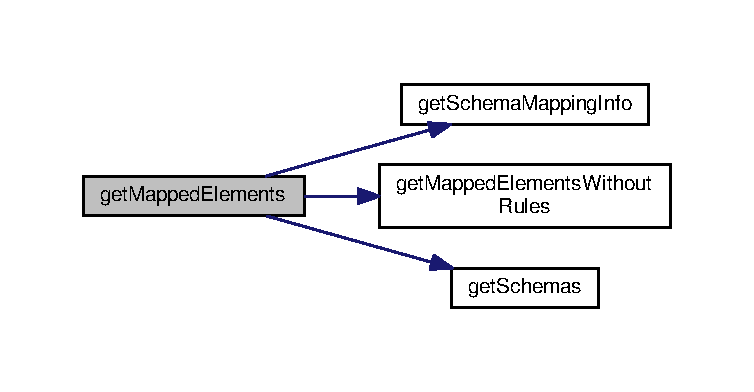
\includegraphics[width=350pt]{namespace_consistency_a489e7863dc1879d02c46deb03793bc03_cgraph}
\end{center}
\end{figure}


\index{Consistency@{Consistency}!get\+Mapped\+Elements\+Without\+Rules@{get\+Mapped\+Elements\+Without\+Rules}}
\index{get\+Mapped\+Elements\+Without\+Rules@{get\+Mapped\+Elements\+Without\+Rules}!Consistency@{Consistency}}
\subsubsection[{\texorpdfstring{get\+Mapped\+Elements\+Without\+Rules(\$mapping)}{getMappedElementsWithoutRules($mapping)}}]{\setlength{\rightskip}{0pt plus 5cm}Consistency\textbackslash{}get\+Mapped\+Elements\+Without\+Rules (
\begin{DoxyParamCaption}
\item[{}]{\$mapping}
\end{DoxyParamCaption}
)}\hypertarget{namespace_consistency_a2be2339d3806b3febbdb87bd1c27e603}{}\label{namespace_consistency_a2be2339d3806b3febbdb87bd1c27e603}
get elements, without associated rules


\begin{DoxyParams}[1]{Parameters}
string & {\em \$mapping} & \\
\hline
\end{DoxyParams}
\begin{DoxyReturn}{Returns}
array 
\end{DoxyReturn}


Definition at line 102 of file check\+Rules.\+php.



Here is the caller graph for this function\+:\nopagebreak
\begin{figure}[H]
\begin{center}
\leavevmode
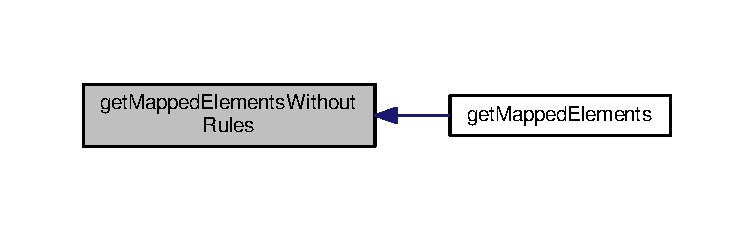
\includegraphics[width=350pt]{namespace_consistency_a2be2339d3806b3febbdb87bd1c27e603_icgraph}
\end{center}
\end{figure}


\index{Consistency@{Consistency}!get\+Rule\+Info@{get\+Rule\+Info}}
\index{get\+Rule\+Info@{get\+Rule\+Info}!Consistency@{Consistency}}
\subsubsection[{\texorpdfstring{get\+Rule\+Info(\$concept, \$mapping)}{getRuleInfo($concept, $mapping)}}]{\setlength{\rightskip}{0pt plus 5cm}Consistency\textbackslash{}get\+Rule\+Info (
\begin{DoxyParamCaption}
\item[{}]{\$concept, }
\item[{}]{\$mapping}
\end{DoxyParamCaption}
)}\hypertarget{namespace_consistency_a1e0e4ba06ca24d6cd0bda99a99ce9f5d}{}\label{namespace_consistency_a1e0e4ba06ca24d6cd0bda99a99ce9f5d}
get rule infos for given Concept and Schema mapping


\begin{DoxyParams}[1]{Parameters}
string & {\em \$concept} & source element \\
\hline
string & {\em \$mapping} & schema mapping \\
\hline
\end{DoxyParams}
\begin{DoxyReturn}{Returns}
array 
\end{DoxyReturn}


Definition at line 70 of file check\+For\+Errors.\+php.



Here is the call graph for this function\+:\nopagebreak
\begin{figure}[H]
\begin{center}
\leavevmode
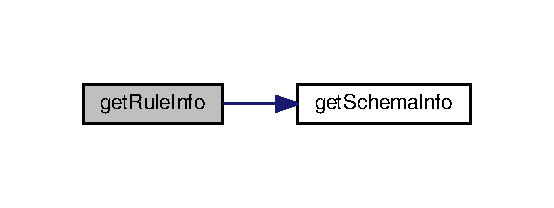
\includegraphics[width=266pt]{namespace_consistency_a1e0e4ba06ca24d6cd0bda99a99ce9f5d_cgraph}
\end{center}
\end{figure}


\index{Consistency@{Consistency}!get\+Schema\+Info@{get\+Schema\+Info}}
\index{get\+Schema\+Info@{get\+Schema\+Info}!Consistency@{Consistency}}
\subsubsection[{\texorpdfstring{get\+Schema\+Info(\$schema)}{getSchemaInfo($schema)}}]{\setlength{\rightskip}{0pt plus 5cm}Consistency\textbackslash{}get\+Schema\+Info (
\begin{DoxyParamCaption}
\item[{}]{\$schema}
\end{DoxyParamCaption}
)}\hypertarget{namespace_consistency_a4359f5b054e4c15acb39a611e29e17c8}{}\label{namespace_consistency_a4359f5b054e4c15acb39a611e29e17c8}
get schema infos for given Schema


\begin{DoxyParams}[1]{Parameters}
string & {\em \$schema} & \\
\hline
\end{DoxyParams}
\begin{DoxyReturn}{Returns}
array 
\end{DoxyReturn}


Definition at line 51 of file check\+For\+Errors.\+php.



Here is the caller graph for this function\+:\nopagebreak
\begin{figure}[H]
\begin{center}
\leavevmode
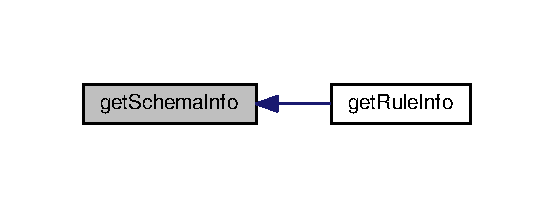
\includegraphics[width=266pt]{namespace_consistency_a4359f5b054e4c15acb39a611e29e17c8_icgraph}
\end{center}
\end{figure}


\index{Consistency@{Consistency}!get\+Schema\+Mapping\+Info@{get\+Schema\+Mapping\+Info}}
\index{get\+Schema\+Mapping\+Info@{get\+Schema\+Mapping\+Info}!Consistency@{Consistency}}
\subsubsection[{\texorpdfstring{get\+Schema\+Mapping\+Info(\$mapping)}{getSchemaMappingInfo($mapping)}}]{\setlength{\rightskip}{0pt plus 5cm}Consistency\textbackslash{}get\+Schema\+Mapping\+Info (
\begin{DoxyParamCaption}
\item[{}]{\$mapping}
\end{DoxyParamCaption}
)}\hypertarget{namespace_consistency_a9bf0ee2da6d3a74ee9dbfcf73ae9842e}{}\label{namespace_consistency_a9bf0ee2da6d3a74ee9dbfcf73ae9842e}
get Schema Mapping Info


\begin{DoxyParams}[1]{Parameters}
string & {\em \$mapping} & \\
\hline
\end{DoxyParams}
\begin{DoxyReturn}{Returns}
array 
\end{DoxyReturn}


Definition at line 68 of file check\+Rules.\+php.



Here is the caller graph for this function\+:\nopagebreak
\begin{figure}[H]
\begin{center}
\leavevmode
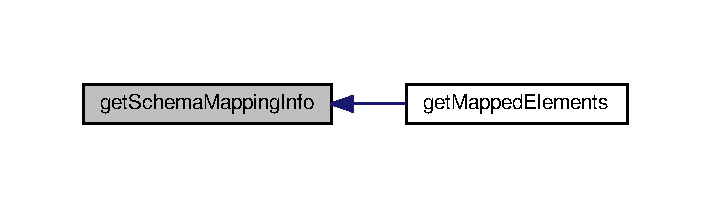
\includegraphics[width=341pt]{namespace_consistency_a9bf0ee2da6d3a74ee9dbfcf73ae9842e_icgraph}
\end{center}
\end{figure}


\index{Consistency@{Consistency}!get\+Schema\+Mappings@{get\+Schema\+Mappings}}
\index{get\+Schema\+Mappings@{get\+Schema\+Mappings}!Consistency@{Consistency}}
\subsubsection[{\texorpdfstring{get\+Schema\+Mappings(\$mapping)}{getSchemaMappings($mapping)}}]{\setlength{\rightskip}{0pt plus 5cm}Consistency\textbackslash{}get\+Schema\+Mappings (
\begin{DoxyParamCaption}
\item[{}]{\$mapping}
\end{DoxyParamCaption}
)}\hypertarget{namespace_consistency_aa98f8a888d842fcaefeca3407c10435c}{}\label{namespace_consistency_aa98f8a888d842fcaefeca3407c10435c}
get Schema Mappings

\begin{DoxyRefDesc}{Todo}
\item[\hyperlink{todo__todo000006}{Todo}]add parameter dataset, and restrict result to supported Schemas \end{DoxyRefDesc}

\begin{DoxyParams}[1]{Parameters}
string & {\em \$mapping} & \\
\hline
\end{DoxyParams}
\begin{DoxyReturn}{Returns}
string J\+S\+ON object 
\end{DoxyReturn}


Definition at line 40 of file get\+Schema\+Mappings.\+php.

\index{Consistency@{Consistency}!get\+Schemas@{get\+Schemas}}
\index{get\+Schemas@{get\+Schemas}!Consistency@{Consistency}}
\subsubsection[{\texorpdfstring{get\+Schemas()}{getSchemas()}}]{\setlength{\rightskip}{0pt plus 5cm}Consistency\textbackslash{}get\+Schemas (
\begin{DoxyParamCaption}
{}
\end{DoxyParamCaption}
)}\hypertarget{namespace_consistency_ac3ce77dc252c4606ec6b0378f5d79ac7}{}\label{namespace_consistency_ac3ce77dc252c4606ec6b0378f5d79ac7}
get Schemas

\begin{DoxyReturn}{Returns}
array 
\end{DoxyReturn}


Definition at line 46 of file check\+Rules.\+php.



\subsection{Variable Documentation}
\index{Consistency@{Consistency}!\$aconcept@{\$aconcept}}
\index{\$aconcept@{\$aconcept}!Consistency@{Consistency}}
\subsubsection[{\texorpdfstring{\$aconcept}{$aconcept}}]{\setlength{\rightskip}{0pt plus 5cm}\$aconcept = explode(\char`\"{}/\char`\"{}, \$concept)}\hypertarget{namespace_consistency_a7ab539c1f2610226e15527ae9f66d1b4}{}\label{namespace_consistency_a7ab539c1f2610226e15527ae9f66d1b4}
build array of parts of a concept, auxiliary step to add schema prefix to each part 

Definition at line 54 of file get\+Example\+Values.\+php.

\index{Consistency@{Consistency}!\$concept\+\_\+xpath@{\$concept\+\_\+xpath}}
\index{\$concept\+\_\+xpath@{\$concept\+\_\+xpath}!Consistency@{Consistency}}
\subsubsection[{\texorpdfstring{\$concept\+\_\+xpath}{$concept_xpath}}]{\setlength{\rightskip}{0pt plus 5cm}\$concept\+\_\+xpath = implode(\char`\"{}/abcd\+:\char`\"{}, \$aconcept)}\hypertarget{namespace_consistency_a6de4812dd264c558f2dadf3ae20b1da2}{}\label{namespace_consistency_a6de4812dd264c558f2dadf3ae20b1da2}
\begin{DoxyRefDesc}{Todo}
\item[\hyperlink{todo__todo000005}{Todo}]compute element xpath with correct prefix for given schema \end{DoxyRefDesc}


Definition at line 58 of file get\+Example\+Values.\+php.

\index{Consistency@{Consistency}!\$dsa@{\$dsa}}
\index{\$dsa@{\$dsa}!Consistency@{Consistency}}
\subsubsection[{\texorpdfstring{\$dsa}{$dsa}}]{\setlength{\rightskip}{0pt plus 5cm}\$dsa = \$\+\_\+\+R\+E\+Q\+U\+E\+ST\mbox{[}\char`\"{}dsa\char`\"{}\mbox{]}}\hypertarget{namespace_consistency_aca6ad28ee812df74bbd827a9d244055e}{}\label{namespace_consistency_aca6ad28ee812df74bbd827a9d244055e}
e.\+g. mfn\+\_\+pal 

Definition at line 36 of file check\+Rules.\+php.

\index{Consistency@{Consistency}!\$filter@{\$filter}}
\index{\$filter@{\$filter}!Consistency@{Consistency}}
\subsubsection[{\texorpdfstring{\$filter}{$filter}}]{\setlength{\rightskip}{0pt plus 5cm}\$filter = filter\+\_\+input(I\+N\+P\+U\+T\+\_\+\+G\+ET, \textquotesingle{}filter\textquotesingle{})}\hypertarget{namespace_consistency_aac53bdb48bdd96ff9c20e2a86f48ce5f}{}\label{namespace_consistency_aac53bdb48bdd96ff9c20e2a86f48ce5f}
e.\+g. $<$filter$>$$<$like path=\char`\"{}/\+Data\+Sets/\+Data\+Set/\+Metadata/\+Description/\+Representation/\+Title\char`\"{}$>$E\+D\+IT -\/ A\+T\+BI in Spreewald (Germany)$<$/like$>$$<$/filter$>$ 

Definition at line 42 of file cardinal\+Concept.\+php.

\index{Consistency@{Consistency}!\$id\+Provider@{\$id\+Provider}}
\index{\$id\+Provider@{\$id\+Provider}!Consistency@{Consistency}}
\subsubsection[{\texorpdfstring{\$id\+Provider}{$idProvider}}]{\setlength{\rightskip}{0pt plus 5cm}\$id\+Provider = \$\+\_\+\+G\+ET\mbox{[}\char`\"{}provider\char`\"{}\mbox{]}}\hypertarget{namespace_consistency_a7c95ff52e91cdd46d783255e270c6d7f}{}\label{namespace_consistency_a7c95ff52e91cdd46d783255e270c6d7f}
e.\+g. MfN 

Definition at line 43 of file index.\+php.

\index{Consistency@{Consistency}!\$mapping@{\$mapping}}
\index{\$mapping@{\$mapping}!Consistency@{Consistency}}
\subsubsection[{\texorpdfstring{\$mapping}{$mapping}}]{\setlength{\rightskip}{0pt plus 5cm}\$mapping = \$\+\_\+\+R\+E\+Q\+U\+E\+ST\mbox{[}\char`\"{}mapping\char`\"{}\mbox{]}}\hypertarget{namespace_consistency_a2c93d0b89d7eadb6b8dfb7c83bc991f9}{}\label{namespace_consistency_a2c93d0b89d7eadb6b8dfb7c83bc991f9}
e.\+g. abcd\+\_\+pansimple 

Definition at line 40 of file check\+For\+Errors.\+php.

\index{Consistency@{Consistency}!\$source\+\_\+schema@{\$source\+\_\+schema}}
\index{\$source\+\_\+schema@{\$source\+\_\+schema}!Consistency@{Consistency}}
\subsubsection[{\texorpdfstring{\$source\+\_\+schema}{$source_schema}}]{\setlength{\rightskip}{0pt plus 5cm}\$source\+\_\+schema = \$\+\_\+\+G\+ET\mbox{[}\char`\"{}source\+\_\+schema\char`\"{}\mbox{]}}\hypertarget{namespace_consistency_ae760b4b690dd68b19e3624cdaddb5ad1}{}\label{namespace_consistency_ae760b4b690dd68b19e3624cdaddb5ad1}
e.\+g. A\+B\+C\+D2.\+06 

Definition at line 63 of file index.\+php.

\index{Consistency@{Consistency}!\$target\+\_\+schema@{\$target\+\_\+schema}}
\index{\$target\+\_\+schema@{\$target\+\_\+schema}!Consistency@{Consistency}}
\subsubsection[{\texorpdfstring{\$target\+\_\+schema}{$target_schema}}]{\setlength{\rightskip}{0pt plus 5cm}\$target\+\_\+schema = \$\+\_\+\+G\+ET\mbox{[}\char`\"{}target\+\_\+schema\char`\"{}\mbox{]}}\hypertarget{namespace_consistency_a43945d5f5c2b8601a121f40a2db7b5b2}{}\label{namespace_consistency_a43945d5f5c2b8601a121f40a2db7b5b2}
e.\+g. pansimple 

Definition at line 67 of file index.\+php.


\hypertarget{namespace_webservices}{}\section{Webservices Namespace Reference}
\label{namespace_webservices}\index{Webservices@{Webservices}}
\subsection*{Functions}
\begin{DoxyCompactItemize}
\item 
\hyperlink{namespace_webservices_a4d1a72eadb36c3dbc90614be4c669e6d}{get\+Citations} (\$id\+D\+SA)
\item 
\hyperlink{namespace_webservices_a43ab3c5a3b6ac98afa231d961ffe33f9}{get\+Data\+Sources} (\$id\+Provider)
\item 
\hyperlink{namespace_webservices_a56703e6dd42e07b8734efeb0f2f7bd88}{get\+Provider\+Info} (\$id\+Provider)
\item 
\hyperlink{namespace_webservices_ad27d0dcb2a954ed5890f6c44c37e3d80}{get\+Landingpages} (\$provider, \$dsa, \$filter, \$inst, \$col, \$cat)
\item 
\hyperlink{namespace_webservices_a982728deb9ddc1d58b4496ef46159b73}{get\+Providers} (\$id, \$name)
\item 
\hyperlink{namespace_webservices_ac8ab1673965ee4402764681d199621d2}{get\+Total\+Records} (\$id\+D\+SA)
\item 
\hyperlink{namespace_webservices_ae993bcd484dd56a7995b75671c97c0ba}{get\+Useful\+Links} (\$id\+D\+SA, \$id\+Provider)
\item 
\hyperlink{namespace_webservices_a120cf6b05d30673945818b2e9dadcba4}{get\+Xml\+Archives} (\$id\+Provider, \$id\+D\+SA)
\end{DoxyCompactItemize}


\subsection{Detailed Description}
Bio\+C\+A\+Se Monitor 2.\+1 \begin{DoxyCopyright}{Copyright}
(C) 2013-\/2018 www.\+museumfuernaturkunde.\+berlin 
\end{DoxyCopyright}
\begin{DoxyAuthor}{Author}
\href{mailto:thomas.pfuhl@mfn.berlin}{\tt thomas.\+pfuhl@mfn.\+berlin} based on Version 1.\+4 written by \href{mailto:falko.gloeckler@mfn.berlin}{\tt falko.\+gloeckler@mfn.\+berlin} 
\end{DoxyAuthor}


\subsection{Function Documentation}
\index{Webservices@{Webservices}!get\+Citations@{get\+Citations}}
\index{get\+Citations@{get\+Citations}!Webservices@{Webservices}}
\subsubsection[{\texorpdfstring{get\+Citations(\$id\+D\+S\+A)}{getCitations($idDSA)}}]{\setlength{\rightskip}{0pt plus 5cm}Webservices\textbackslash{}get\+Citations (
\begin{DoxyParamCaption}
\item[{}]{\$id\+D\+SA}
\end{DoxyParamCaption}
)}\hypertarget{namespace_webservices_a4d1a72eadb36c3dbc90614be4c669e6d}{}\label{namespace_webservices_a4d1a72eadb36c3dbc90614be4c669e6d}
get Citation text of given Data Set, not yet implemented


\begin{DoxyParams}{Parameters}
{\em \$id\+D\+SA} & \\
\hline
\end{DoxyParams}
\begin{DoxyReturn}{Returns}
json 
\end{DoxyReturn}


Definition at line 41 of file index.\+php.

\index{Webservices@{Webservices}!get\+Data\+Sources@{get\+Data\+Sources}}
\index{get\+Data\+Sources@{get\+Data\+Sources}!Webservices@{Webservices}}
\subsubsection[{\texorpdfstring{get\+Data\+Sources(\$id\+Provider)}{getDataSources($idProvider)}}]{\setlength{\rightskip}{0pt plus 5cm}Webservices\textbackslash{}get\+Data\+Sources (
\begin{DoxyParamCaption}
\item[{}]{\$id\+Provider}
\end{DoxyParamCaption}
)}\hypertarget{namespace_webservices_a43ab3c5a3b6ac98afa231d961ffe33f9}{}\label{namespace_webservices_a43ab3c5a3b6ac98afa231d961ffe33f9}
get Datasources


\begin{DoxyParams}{Parameters}
{\em \$id\+Provider} & \\
\hline
\end{DoxyParams}
\begin{DoxyReturn}{Returns}
json 
\end{DoxyReturn}


Definition at line 38 of file index.\+php.

\index{Webservices@{Webservices}!get\+Landingpages@{get\+Landingpages}}
\index{get\+Landingpages@{get\+Landingpages}!Webservices@{Webservices}}
\subsubsection[{\texorpdfstring{get\+Landingpages(\$provider, \$dsa, \$filter, \$inst, \$col, \$cat)}{getLandingpages($provider, $dsa, $filter, $inst, $col, $cat)}}]{\setlength{\rightskip}{0pt plus 5cm}Webservices\textbackslash{}get\+Landingpages (
\begin{DoxyParamCaption}
\item[{}]{\$provider, }
\item[{}]{\$dsa, }
\item[{}]{\$filter, }
\item[{}]{\$inst, }
\item[{}]{\$col, }
\item[{}]{\$cat}
\end{DoxyParamCaption}
)}\hypertarget{namespace_webservices_ad27d0dcb2a954ed5890f6c44c37e3d80}{}\label{namespace_webservices_ad27d0dcb2a954ed5890f6c44c37e3d80}
get U\+R\+Ls for landing pages


\begin{DoxyParams}[1]{Parameters}
array & {\em \$provider} & \\
\hline
int & {\em \$dsa} & \\
\hline
string & {\em \$filter} & \\
\hline
string & {\em \$inst} & \\
\hline
string & {\em \$col} & \\
\hline
string & {\em \$cat} & \\
\hline
\end{DoxyParams}
\begin{DoxyReturn}{Returns}
json 
\end{DoxyReturn}


Definition at line 81 of file index.\+php.



Here is the call graph for this function\+:\nopagebreak
\begin{figure}[H]
\begin{center}
\leavevmode
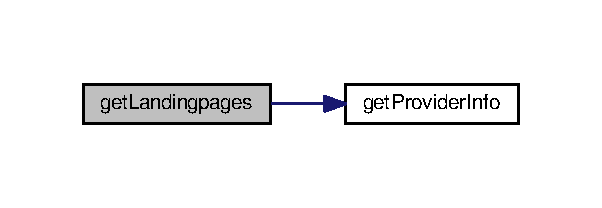
\includegraphics[width=289pt]{namespace_webservices_ad27d0dcb2a954ed5890f6c44c37e3d80_cgraph}
\end{center}
\end{figure}


\index{Webservices@{Webservices}!get\+Provider\+Info@{get\+Provider\+Info}}
\index{get\+Provider\+Info@{get\+Provider\+Info}!Webservices@{Webservices}}
\subsubsection[{\texorpdfstring{get\+Provider\+Info(\$id\+Provider)}{getProviderInfo($idProvider)}}]{\setlength{\rightskip}{0pt plus 5cm}Webservices\textbackslash{}get\+Provider\+Info (
\begin{DoxyParamCaption}
\item[{}]{\$id\+Provider}
\end{DoxyParamCaption}
)}\hypertarget{namespace_webservices_a56703e6dd42e07b8734efeb0f2f7bd88}{}\label{namespace_webservices_a56703e6dd42e07b8734efeb0f2f7bd88}
get Infos about Data Provider


\begin{DoxyParams}{Parameters}
{\em \$id\+Provider} & \\
\hline
\end{DoxyParams}
\begin{DoxyReturn}{Returns}
array 
\end{DoxyReturn}


Definition at line 50 of file index.\+php.



Here is the caller graph for this function\+:\nopagebreak
\begin{figure}[H]
\begin{center}
\leavevmode
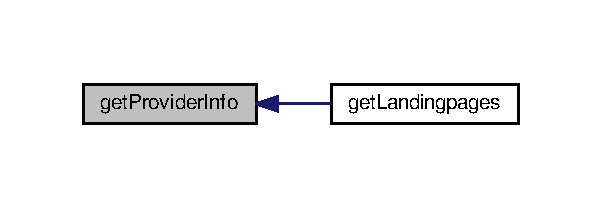
\includegraphics[width=289pt]{namespace_webservices_a56703e6dd42e07b8734efeb0f2f7bd88_icgraph}
\end{center}
\end{figure}


\index{Webservices@{Webservices}!get\+Providers@{get\+Providers}}
\index{get\+Providers@{get\+Providers}!Webservices@{Webservices}}
\subsubsection[{\texorpdfstring{get\+Providers(\$id, \$name)}{getProviders($id, $name)}}]{\setlength{\rightskip}{0pt plus 5cm}Webservices\textbackslash{}get\+Providers (
\begin{DoxyParamCaption}
\item[{}]{\$id, }
\item[{}]{\$name}
\end{DoxyParamCaption}
)}\hypertarget{namespace_webservices_a982728deb9ddc1d58b4496ef46159b73}{}\label{namespace_webservices_a982728deb9ddc1d58b4496ef46159b73}
get providers 
\begin{DoxyParams}[1]{Parameters}
int & {\em \$id} & \\
\hline
string & {\em \$name} & \\
\hline
\end{DoxyParams}


Definition at line 36 of file index.\+php.



Here is the call graph for this function\+:\nopagebreak
\begin{figure}[H]
\begin{center}
\leavevmode
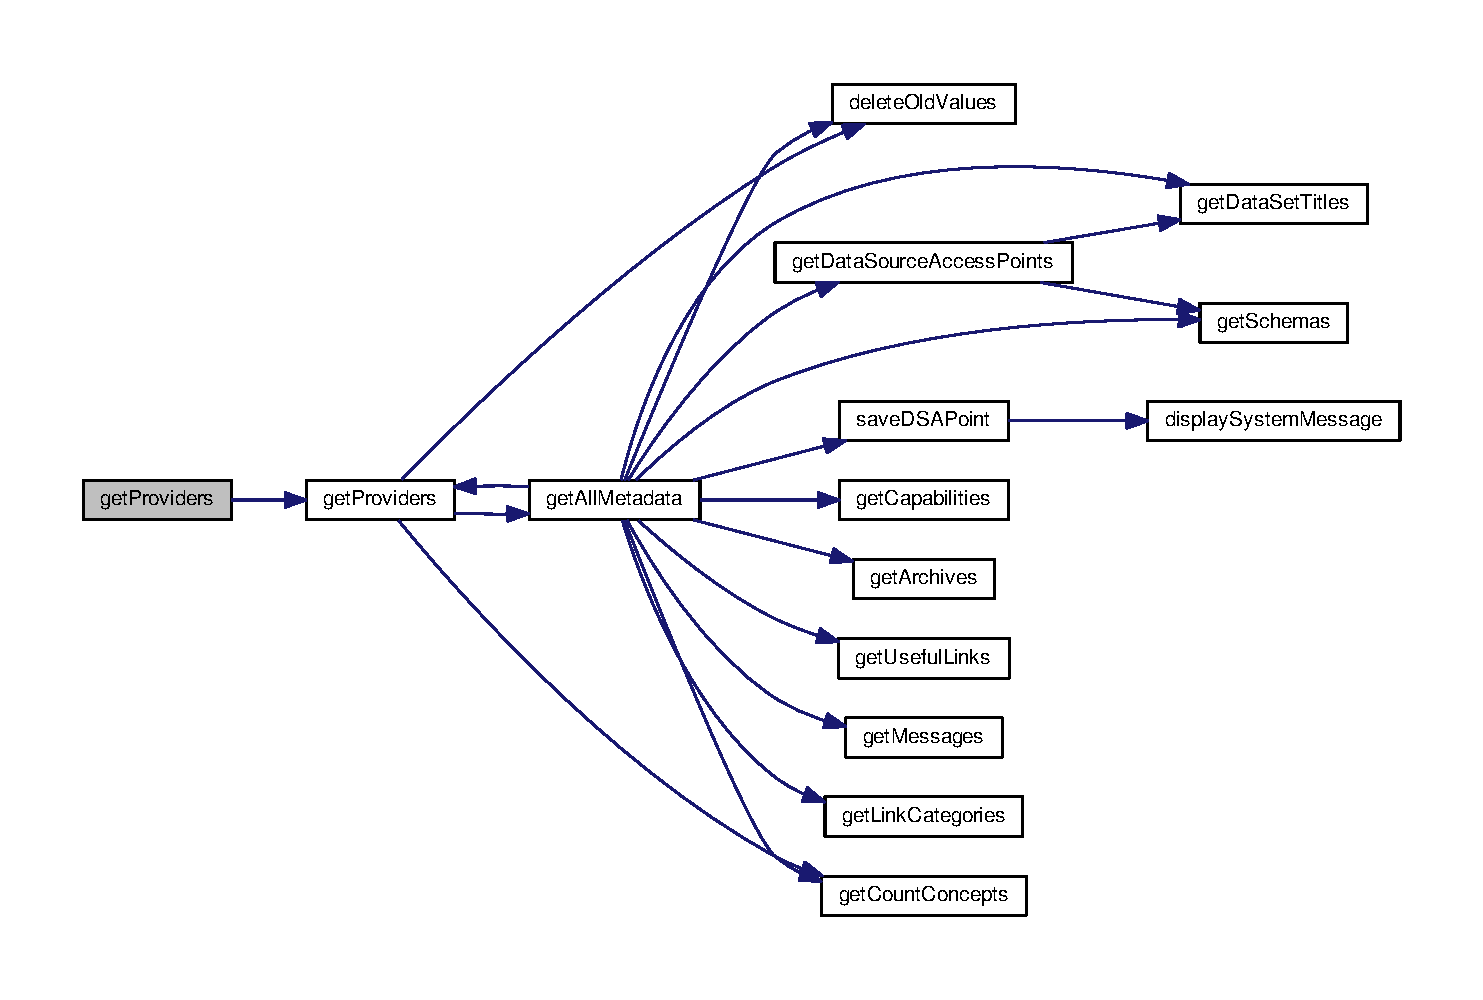
\includegraphics[width=350pt]{namespace_webservices_a982728deb9ddc1d58b4496ef46159b73_cgraph}
\end{center}
\end{figure}


\index{Webservices@{Webservices}!get\+Total\+Records@{get\+Total\+Records}}
\index{get\+Total\+Records@{get\+Total\+Records}!Webservices@{Webservices}}
\subsubsection[{\texorpdfstring{get\+Total\+Records(\$id\+D\+S\+A)}{getTotalRecords($idDSA)}}]{\setlength{\rightskip}{0pt plus 5cm}Webservices\textbackslash{}get\+Total\+Records (
\begin{DoxyParamCaption}
\item[{}]{\$id\+D\+SA}
\end{DoxyParamCaption}
)}\hypertarget{namespace_webservices_ac8ab1673965ee4402764681d199621d2}{}\label{namespace_webservices_ac8ab1673965ee4402764681d199621d2}
get total records for given D\+SA not yet implemented


\begin{DoxyParams}{Parameters}
{\em \$id\+D\+SA} & \\
\hline
\end{DoxyParams}
\begin{DoxyReturn}{Returns}
json 
\end{DoxyReturn}


Definition at line 38 of file index.\+php.

\index{Webservices@{Webservices}!get\+Useful\+Links@{get\+Useful\+Links}}
\index{get\+Useful\+Links@{get\+Useful\+Links}!Webservices@{Webservices}}
\subsubsection[{\texorpdfstring{get\+Useful\+Links(\$id\+D\+S\+A, \$id\+Provider)}{getUsefulLinks($idDSA, $idProvider)}}]{\setlength{\rightskip}{0pt plus 5cm}Webservices\textbackslash{}get\+Useful\+Links (
\begin{DoxyParamCaption}
\item[{}]{\$id\+D\+SA, }
\item[{}]{\$id\+Provider}
\end{DoxyParamCaption}
)}\hypertarget{namespace_webservices_ae993bcd484dd56a7995b75671c97c0ba}{}\label{namespace_webservices_ae993bcd484dd56a7995b75671c97c0ba}
webservice get useful links


\begin{DoxyParams}{Parameters}
{\em \$id\+D\+SA} & \\
\hline
{\em \$id\+Provider} & \\
\hline
\end{DoxyParams}
\begin{DoxyReturn}{Returns}
json 
\end{DoxyReturn}


Definition at line 37 of file index.\+php.

\index{Webservices@{Webservices}!get\+Xml\+Archives@{get\+Xml\+Archives}}
\index{get\+Xml\+Archives@{get\+Xml\+Archives}!Webservices@{Webservices}}
\subsubsection[{\texorpdfstring{get\+Xml\+Archives(\$id\+Provider, \$id\+D\+S\+A)}{getXmlArchives($idProvider, $idDSA)}}]{\setlength{\rightskip}{0pt plus 5cm}Webservices\textbackslash{}get\+Xml\+Archives (
\begin{DoxyParamCaption}
\item[{}]{\$id\+Provider, }
\item[{}]{\$id\+D\+SA}
\end{DoxyParamCaption}
)}\hypertarget{namespace_webservices_a120cf6b05d30673945818b2e9dadcba4}{}\label{namespace_webservices_a120cf6b05d30673945818b2e9dadcba4}
get X\+ML Archives


\begin{DoxyParams}[1]{Parameters}
int & {\em \$id\+Provider} & \\
\hline
int & {\em \$id\+D\+SA} & \\
\hline
\end{DoxyParams}
\begin{DoxyReturn}{Returns}
json 
\end{DoxyReturn}


Definition at line 31 of file index.\+php.


\chapter{Data Structure Documentation}
\hypertarget{class_bms_1_1_bms}{}\section{Bms Class Reference}
\label{class_bms_1_1_bms}\index{Bms@{Bms}}
\subsection*{Public Member Functions}
\begin{DoxyCompactItemize}
\item 
\hyperlink{class_bms_1_1_bms_abbd2b270b5a2e822a12646da90c6e48e}{get\+Schema} (\$schema)
\item 
\hyperlink{class_bms_1_1_bms_aad36f7a0d237b521e0c4cc4482895413}{get\+Concepts} (\$id\+Provider)
\item 
\hyperlink{class_bms_1_1_bms_a4ae0faba305bd7f8f82efc796a983b09}{get\+Current\+Records} (\$provider\+Id, \$schema, \$url, \$filter, \$nocache)
\item 
\hyperlink{class_bms_1_1_bms_af007633bad4e22ba700d331292e06fde}{get\+Count\+Concepts} (\$provider\+Id, \$schema, \$url, \$concept, \$specifier, \$filter, \$nocache)
\item 
\hyperlink{class_bms_1_1_bms_ae49caba006e4fd1521d7f96f427ce56a}{get\+Citation} (\$provider\+Id, \$url, \$filter, \$cached=1, \$concept=\char`\"{}/Data\+Sets/Data\+Set/Metadata/I\+P\+R\+Statements/Citations/Citation/Text\char`\"{})
\item 
\hyperlink{class_bms_1_1_bms_a5871c187d76524a84c7fed6dcc3d5169}{get\+Provider\+Main\+Data} (\$id\+Provider)
\item 
\hyperlink{class_bms_1_1_bms_aec5f7b55928d9eb969567ab87ea9e021}{front\+Controller} (\$route)
\item 
\hyperlink{class_bms_1_1_bms_a24b2edfc6aae484d67fbd177cf10e1b1}{get\+Providers} ()
\item 
\hyperlink{class_bms_1_1_bms_a7347b0b89cca1d7604e93f5b5e896fc4}{get\+Messages} ()
\end{DoxyCompactItemize}
\subsection*{Data Fields}
\begin{DoxyCompactItemize}
\item 
\hyperlink{class_bms_1_1_bms_a8d1821dbc83e2d0353770ec855a9621c}{\$debugmode} = \hyperlink{namespace_bms_a7af7ef3e15183adae80bfc7cf0272937}{D\+E\+B\+U\+G\+M\+O\+DE}
\item 
\hyperlink{class_bms_1_1_bms_abfac2de1f5278c24154a318274419e69}{\$custom\+\_\+layout} = 0
\item 
\hyperlink{class_bms_1_1_bms_abf17cb2dba2ed17cb28aa5f37deb5293}{\$message} = \char`\"{}\char`\"{}
\end{DoxyCompactItemize}


\subsection{Detailed Description}
class definition of the Bio\+C\+A\+Se Monitor Service 

Definition at line 43 of file index.\+php.



\subsection{Member Function Documentation}
\index{Bms\+::\+Bms@{Bms\+::\+Bms}!front\+Controller@{front\+Controller}}
\index{front\+Controller@{front\+Controller}!Bms\+::\+Bms@{Bms\+::\+Bms}}
\subsubsection[{\texorpdfstring{front\+Controller(\$route)}{frontController($route)}}]{\setlength{\rightskip}{0pt plus 5cm}front\+Controller (
\begin{DoxyParamCaption}
\item[{}]{\$route}
\end{DoxyParamCaption}
)}\hypertarget{class_bms_1_1_bms_aec5f7b55928d9eb969567ab87ea9e021}{}\label{class_bms_1_1_bms_aec5f7b55928d9eb969567ab87ea9e021}
simple front controller with static routing


\begin{DoxyParams}{Parameters}
{\em \$route} & \\
\hline
\end{DoxyParams}


Definition at line 714 of file index.\+php.



Here is the call graph for this function\+:\nopagebreak
\begin{figure}[H]
\begin{center}
\leavevmode
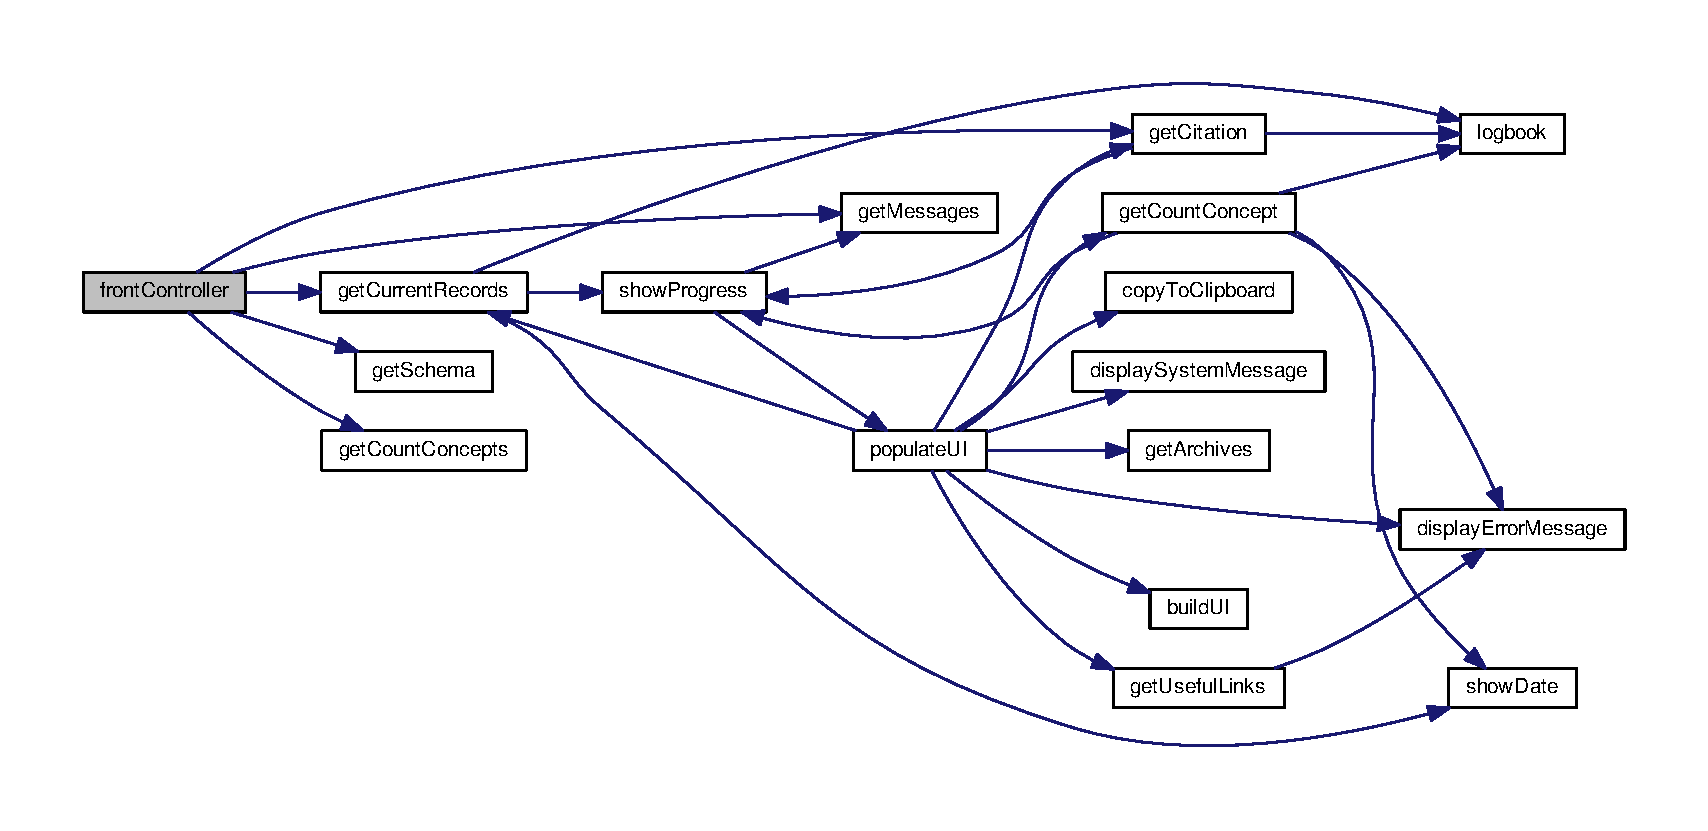
\includegraphics[width=350pt]{class_bms_1_1_bms_aec5f7b55928d9eb969567ab87ea9e021_cgraph}
\end{center}
\end{figure}


\index{Bms\+::\+Bms@{Bms\+::\+Bms}!get\+Citation@{get\+Citation}}
\index{get\+Citation@{get\+Citation}!Bms\+::\+Bms@{Bms\+::\+Bms}}
\subsubsection[{\texorpdfstring{get\+Citation(\$provider\+Id, \$url, \$filter, \$cached=1, \$concept=""/\+Data\+Sets/\+Data\+Set/\+Metadata/\+I\+P\+R\+Statements/\+Citations/\+Citation/\+Text"")}{getCitation($providerId, $url, $filter, $cached=1, $concept="/DataSets/DataSet/Metadata/IPRStatements/Citations/Citation/Text")}}]{\setlength{\rightskip}{0pt plus 5cm}get\+Citation (
\begin{DoxyParamCaption}
\item[{}]{\$provider\+Id, }
\item[{}]{\$url, }
\item[{}]{\$filter, }
\item[{}]{\$cached = {\ttfamily 1}, }
\item[{}]{\$concept = {\ttfamily \char`\"{}/DataSets/DataSet/Metadata/IPRStatements/Citations/Citation/Text\char`\"{}}}
\end{DoxyParamCaption}
)}\hypertarget{class_bms_1_1_bms_ae49caba006e4fd1521d7f96f427ce56a}{}\label{class_bms_1_1_bms_ae49caba006e4fd1521d7f96f427ce56a}
get Citation of a Data\+Set via a B\+PS scan request


\begin{DoxyParams}[1]{Parameters}
string & {\em \$provider\+Id} & \\
\hline
string & {\em \$url} & \\
\hline
string & {\em \$filter} & \\
\hline
int & {\em \$cached} & 0$\vert$1 \\
\hline
string & {\em \$concept} & with default value \char`\"{}/\+Data\+Sets/\+Data\+Set/\+Metadata/\+I\+P\+R\+Statements/\+Citations/\+Citation/\+Text\char`\"{} \\
\hline
\end{DoxyParams}
\begin{DoxyReturn}{Returns}
string json Object 
\end{DoxyReturn}


Definition at line 485 of file index.\+php.

\index{Bms\+::\+Bms@{Bms\+::\+Bms}!get\+Concepts@{get\+Concepts}}
\index{get\+Concepts@{get\+Concepts}!Bms\+::\+Bms@{Bms\+::\+Bms}}
\subsubsection[{\texorpdfstring{get\+Concepts(\$id\+Provider)}{getConcepts($idProvider)}}]{\setlength{\rightskip}{0pt plus 5cm}get\+Concepts (
\begin{DoxyParamCaption}
\item[{}]{\$id\+Provider}
\end{DoxyParamCaption}
)}\hypertarget{class_bms_1_1_bms_aad36f7a0d237b521e0c4cc4482895413}{}\label{class_bms_1_1_bms_aad36f7a0d237b521e0c4cc4482895413}
get list of all concepts of a given provider, via a DB query


\begin{DoxyParams}[1]{Parameters}
int & {\em \$id\+Provider} & \\
\hline
\end{DoxyParams}
\begin{DoxyReturn}{Returns}
string json Object 
\end{DoxyReturn}


Definition at line 105 of file index.\+php.

\index{Bms\+::\+Bms@{Bms\+::\+Bms}!get\+Count\+Concepts@{get\+Count\+Concepts}}
\index{get\+Count\+Concepts@{get\+Count\+Concepts}!Bms\+::\+Bms@{Bms\+::\+Bms}}
\subsubsection[{\texorpdfstring{get\+Count\+Concepts(\$provider\+Id, \$schema, \$url, \$concept, \$specifier, \$filter, \$nocache)}{getCountConcepts($providerId, $schema, $url, $concept, $specifier, $filter, $nocache)}}]{\setlength{\rightskip}{0pt plus 5cm}get\+Count\+Concepts (
\begin{DoxyParamCaption}
\item[{}]{\$provider\+Id, }
\item[{}]{\$schema, }
\item[{}]{\$url, }
\item[{}]{\$concept, }
\item[{}]{\$specifier, }
\item[{}]{\$filter, }
\item[{}]{\$nocache}
\end{DoxyParamCaption}
)}\hypertarget{class_bms_1_1_bms_af007633bad4e22ba700d331292e06fde}{}\label{class_bms_1_1_bms_af007633bad4e22ba700d331292e06fde}
get number of records satisfying a given concept via a B\+PS search or scan request


\begin{DoxyParams}[1]{Parameters}
string & {\em \$provider\+Id} & \\
\hline
string & {\em \$schema} & \\
\hline
string & {\em \$url} & \\
\hline
string & {\em \$concept} & \\
\hline
int & {\em \$specifier} & bitmap T\+O\+T\+AL=1,D\+I\+S\+T\+I\+N\+CT=2,D\+R\+O\+P\+P\+ED=4 \\
\hline
string & {\em \$filter} & complex filter \\
\hline
int & {\em \$nocache} & 1$\vert$0 \\
\hline
\end{DoxyParams}
\begin{DoxyReturn}{Returns}
string json Object 
\end{DoxyReturn}


Definition at line 291 of file index.\+php.

\index{Bms\+::\+Bms@{Bms\+::\+Bms}!get\+Current\+Records@{get\+Current\+Records}}
\index{get\+Current\+Records@{get\+Current\+Records}!Bms\+::\+Bms@{Bms\+::\+Bms}}
\subsubsection[{\texorpdfstring{get\+Current\+Records(\$provider\+Id, \$schema, \$url, \$filter, \$nocache)}{getCurrentRecords($providerId, $schema, $url, $filter, $nocache)}}]{\setlength{\rightskip}{0pt plus 5cm}get\+Current\+Records (
\begin{DoxyParamCaption}
\item[{}]{\$provider\+Id, }
\item[{}]{\$schema, }
\item[{}]{\$url, }
\item[{}]{\$filter, }
\item[{}]{\$nocache}
\end{DoxyParamCaption}
)}\hypertarget{class_bms_1_1_bms_a4ae0faba305bd7f8f82efc796a983b09}{}\label{class_bms_1_1_bms_a4ae0faba305bd7f8f82efc796a983b09}
get Number of Current Records via a B\+PS search request


\begin{DoxyParams}[1]{Parameters}
int & {\em \$provider\+Id} & ID of Data Center \\
\hline
string & {\em \$schema} & Schema \\
\hline
string & {\em \$url} & Query U\+RL \\
\hline
string & {\em \$filter} & complex filter in X\+M\+L-\/format \\
\hline
int & {\em \$nocache} & 1 or 0 \\
\hline
\end{DoxyParams}
\begin{DoxyReturn}{Returns}
string json Object, e.\+g. \{ cardinal\+: 101, error\+: \char`\"{}\char`\"{}, cacheinfo\+: \char`\"{}1467913058\char`\"{}, debuginfo\+: \char`\"{}\char`\"{} \} 
\end{DoxyReturn}


Definition at line 141 of file index.\+php.

\index{Bms\+::\+Bms@{Bms\+::\+Bms}!get\+Messages@{get\+Messages}}
\index{get\+Messages@{get\+Messages}!Bms\+::\+Bms@{Bms\+::\+Bms}}
\subsubsection[{\texorpdfstring{get\+Messages()}{getMessages()}}]{\setlength{\rightskip}{0pt plus 5cm}get\+Messages (
\begin{DoxyParamCaption}
{}
\end{DoxyParamCaption}
)}\hypertarget{class_bms_1_1_bms_a7347b0b89cca1d7604e93f5b5e896fc4}{}\label{class_bms_1_1_bms_a7347b0b89cca1d7604e93f5b5e896fc4}
get system messages

loads system messages into property \char`\"{}message\char`\"{}

\begin{DoxyReturn}{Returns}
string J\+S\+ON object 
\end{DoxyReturn}


Definition at line 849 of file index.\+php.

\index{Bms\+::\+Bms@{Bms\+::\+Bms}!get\+Provider\+Main\+Data@{get\+Provider\+Main\+Data}}
\index{get\+Provider\+Main\+Data@{get\+Provider\+Main\+Data}!Bms\+::\+Bms@{Bms\+::\+Bms}}
\subsubsection[{\texorpdfstring{get\+Provider\+Main\+Data(\$id\+Provider)}{getProviderMainData($idProvider)}}]{\setlength{\rightskip}{0pt plus 5cm}get\+Provider\+Main\+Data (
\begin{DoxyParamCaption}
\item[{}]{\$id\+Provider}
\end{DoxyParamCaption}
)}\hypertarget{class_bms_1_1_bms_a5871c187d76524a84c7fed6dcc3d5169}{}\label{class_bms_1_1_bms_a5871c187d76524a84c7fed6dcc3d5169}
get main data of given provider, via a DB query


\begin{DoxyParams}[1]{Parameters}
int & {\em \$id\+Provider} & \\
\hline
\end{DoxyParams}
\begin{DoxyReturn}{Returns}
object J\+S\+ON object 
\end{DoxyReturn}


Definition at line 650 of file index.\+php.

\index{Bms\+::\+Bms@{Bms\+::\+Bms}!get\+Providers@{get\+Providers}}
\index{get\+Providers@{get\+Providers}!Bms\+::\+Bms@{Bms\+::\+Bms}}
\subsubsection[{\texorpdfstring{get\+Providers()}{getProviders()}}]{\setlength{\rightskip}{0pt plus 5cm}get\+Providers (
\begin{DoxyParamCaption}
{}
\end{DoxyParamCaption}
)}\hypertarget{class_bms_1_1_bms_a24b2edfc6aae484d67fbd177cf10e1b1}{}\label{class_bms_1_1_bms_a24b2edfc6aae484d67fbd177cf10e1b1}
get I\+Ds of providers

\begin{DoxyReturn}{Returns}
array 
\end{DoxyReturn}


Definition at line 827 of file index.\+php.

\index{Bms\+::\+Bms@{Bms\+::\+Bms}!get\+Schema@{get\+Schema}}
\index{get\+Schema@{get\+Schema}!Bms\+::\+Bms@{Bms\+::\+Bms}}
\subsubsection[{\texorpdfstring{get\+Schema(\$schema)}{getSchema($schema)}}]{\setlength{\rightskip}{0pt plus 5cm}get\+Schema (
\begin{DoxyParamCaption}
\item[{}]{\$schema}
\end{DoxyParamCaption}
)}\hypertarget{class_bms_1_1_bms_abbd2b270b5a2e822a12646da90c6e48e}{}\label{class_bms_1_1_bms_abbd2b270b5a2e822a12646da90c6e48e}
get list of all schemas, via a DB query


\begin{DoxyParams}{Parameters}
{\em string} & Schema U\+RN \\
\hline
\end{DoxyParams}
\begin{DoxyReturn}{Returns}
string json Object 
\end{DoxyReturn}


Definition at line 84 of file index.\+php.



\subsection{Field Documentation}
\index{Bms\+::\+Bms@{Bms\+::\+Bms}!\$custom\+\_\+layout@{\$custom\+\_\+layout}}
\index{\$custom\+\_\+layout@{\$custom\+\_\+layout}!Bms\+::\+Bms@{Bms\+::\+Bms}}
\subsubsection[{\texorpdfstring{\$custom\+\_\+layout}{$custom_layout}}]{\setlength{\rightskip}{0pt plus 5cm}\$custom\+\_\+layout = 0}\hypertarget{class_bms_1_1_bms_abfac2de1f5278c24154a318274419e69}{}\label{class_bms_1_1_bms_abfac2de1f5278c24154a318274419e69}
set custom layout mode, omay be overwritten by G\+ET parameter 

Definition at line 53 of file index.\+php.

\index{Bms\+::\+Bms@{Bms\+::\+Bms}!\$debugmode@{\$debugmode}}
\index{\$debugmode@{\$debugmode}!Bms\+::\+Bms@{Bms\+::\+Bms}}
\subsubsection[{\texorpdfstring{\$debugmode}{$debugmode}}]{\setlength{\rightskip}{0pt plus 5cm}\$debugmode = {\bf D\+E\+B\+U\+G\+M\+O\+DE}}\hypertarget{class_bms_1_1_bms_a8d1821dbc83e2d0353770ec855a9621c}{}\label{class_bms_1_1_bms_a8d1821dbc83e2d0353770ec855a9621c}
set debug mode, overwriting constant D\+E\+B\+U\+G\+M\+O\+DE by G\+ET parameter 

Definition at line 48 of file index.\+php.

\index{Bms\+::\+Bms@{Bms\+::\+Bms}!\$message@{\$message}}
\index{\$message@{\$message}!Bms\+::\+Bms@{Bms\+::\+Bms}}
\subsubsection[{\texorpdfstring{\$message}{$message}}]{\setlength{\rightskip}{0pt plus 5cm}\${\bf message} = \char`\"{}\char`\"{}}\hypertarget{class_bms_1_1_bms_abf17cb2dba2ed17cb28aa5f37deb5293}{}\label{class_bms_1_1_bms_abf17cb2dba2ed17cb28aa5f37deb5293}
holds the system messages 

Definition at line 58 of file index.\+php.



The documentation for this class was generated from the following file\+:\begin{DoxyCompactItemize}
\item 
\hyperlink{index_8php}{index.\+php}\end{DoxyCompactItemize}

\chapter{File Documentation}
\hypertarget{add_archive_8php}{}\section{admin/add\+Archive.php File Reference}
\label{add_archive_8php}\index{admin/add\+Archive.\+php@{admin/add\+Archive.\+php}}


backend\+: add an X\+ML Archive  




\subsection{Detailed Description}
Bio\+C\+A\+Se Monitor 2.\+1 \begin{DoxyCopyright}{Copyright}
(C) 2013-\/2018 www.\+museumfuernaturkunde.\+berlin 
\end{DoxyCopyright}
\begin{DoxyAuthor}{Author}
\href{mailto:thomas.pfuhl@mfn.berlin}{\tt thomas.\+pfuhl@mfn.\+berlin} based on Version 1.\+4 written by \href{mailto:falko.gloeckler@mfn.berlin}{\tt falko.\+gloeckler@mfn.\+berlin}
\end{DoxyAuthor}
This program is free software\+: you can redistribute it and/or modify it under the terms of the G\+NU General Public License as published by the Free Software Foundation, either version 3 of the License, or (at your option) any later version.

This program is distributed in the hope that it will be useful, but W\+I\+T\+H\+O\+UT A\+NY W\+A\+R\+R\+A\+N\+TY; without even the implied warranty of M\+E\+R\+C\+H\+A\+N\+T\+A\+B\+I\+L\+I\+TY or F\+I\+T\+N\+E\+SS F\+OR A P\+A\+R\+T\+I\+C\+U\+L\+AR P\+U\+R\+P\+O\+SE. See the G\+NU General Public License for more details.

You should have received a copy of the G\+NU General Public License along with this program. If not, see \href{http://www.gnu.org/licenses/}{\tt http\+://www.\+gnu.\+org/licenses/}. 
\hypertarget{add_count_8php}{}\section{admin/add\+Count.php File Reference}
\label{add_count_8php}\index{admin/add\+Count.\+php@{admin/add\+Count.\+php}}


backend\+: add a Count Concept  




\subsection{Detailed Description}
Bio\+C\+A\+Se Monitor 2.\+1 \begin{DoxyCopyright}{Copyright}
(C) 2013-\/2018 www.\+museumfuernaturkunde.\+berlin 
\end{DoxyCopyright}
\begin{DoxyAuthor}{Author}
\href{mailto:thomas.pfuhl@mfn.berlin}{\tt thomas.\+pfuhl@mfn.\+berlin} based on Version 1.\+4 written by \href{mailto:falko.gloeckler@mfn.berlin}{\tt falko.\+gloeckler@mfn.\+berlin}
\end{DoxyAuthor}
This program is free software\+: you can redistribute it and/or modify it under the terms of the G\+NU General Public License as published by the Free Software Foundation, either version 3 of the License, or (at your option) any later version.

This program is distributed in the hope that it will be useful, but W\+I\+T\+H\+O\+UT A\+NY W\+A\+R\+R\+A\+N\+TY; without even the implied warranty of M\+E\+R\+C\+H\+A\+N\+T\+A\+B\+I\+L\+I\+TY or F\+I\+T\+N\+E\+SS F\+OR A P\+A\+R\+T\+I\+C\+U\+L\+AR P\+U\+R\+P\+O\+SE. See the G\+NU General Public License for more details.

You should have received a copy of the G\+NU General Public License along with this program. If not, see \href{http://www.gnu.org/licenses/}{\tt http\+://www.\+gnu.\+org/licenses/}. 
\hypertarget{add_d_s_a_8php}{}\section{admin/add\+D\+SA.php File Reference}
\label{add_d_s_a_8php}\index{admin/add\+D\+S\+A.\+php@{admin/add\+D\+S\+A.\+php}}


backend\+: add a D\+SA Point  




\subsection{Detailed Description}
Bio\+C\+A\+Se Monitor 2.\+1 \begin{DoxyCopyright}{Copyright}
(C) 2013-\/2018 www.\+museumfuernaturkunde.\+berlin 
\end{DoxyCopyright}
\begin{DoxyAuthor}{Author}
\href{mailto:thomas.pfuhl@mfn.berlin}{\tt thomas.\+pfuhl@mfn.\+berlin} based on Version 1.\+4 written by \href{mailto:falko.gloeckler@mfn.berlin}{\tt falko.\+gloeckler@mfn.\+berlin}
\end{DoxyAuthor}
This program is free software\+: you can redistribute it and/or modify it under the terms of the G\+NU General Public License as published by the Free Software Foundation, either version 3 of the License, or (at your option) any later version.

This program is distributed in the hope that it will be useful, but W\+I\+T\+H\+O\+UT A\+NY W\+A\+R\+R\+A\+N\+TY; without even the implied warranty of M\+E\+R\+C\+H\+A\+N\+T\+A\+B\+I\+L\+I\+TY or F\+I\+T\+N\+E\+SS F\+OR A P\+A\+R\+T\+I\+C\+U\+L\+AR P\+U\+R\+P\+O\+SE. See the G\+NU General Public License for more details.

You should have received a copy of the G\+NU General Public License along with this program. If not, see \href{http://www.gnu.org/licenses/}{\tt http\+://www.\+gnu.\+org/licenses/}. 
\hypertarget{add_useful_link_8php}{}\section{admin/add\+Useful\+Link.php File Reference}
\label{add_useful_link_8php}\index{admin/add\+Useful\+Link.\+php@{admin/add\+Useful\+Link.\+php}}


backend\+: add a useful Link  




\subsection{Detailed Description}
Bio\+C\+A\+Se Monitor 2.\+1 \begin{DoxyCopyright}{Copyright}
(C) 2013-\/2018 www.\+museumfuernaturkunde.\+berlin 
\end{DoxyCopyright}
\begin{DoxyAuthor}{Author}
\href{mailto:thomas.pfuhl@mfn.berlin}{\tt thomas.\+pfuhl@mfn.\+berlin} based on Version 1.\+4 written by \href{mailto:falko.gloeckler@mfn.berlin}{\tt falko.\+gloeckler@mfn.\+berlin}
\end{DoxyAuthor}
This program is free software\+: you can redistribute it and/or modify it under the terms of the G\+NU General Public License as published by the Free Software Foundation, either version 3 of the License, or (at your option) any later version.

This program is distributed in the hope that it will be useful, but W\+I\+T\+H\+O\+UT A\+NY W\+A\+R\+R\+A\+N\+TY; without even the implied warranty of M\+E\+R\+C\+H\+A\+N\+T\+A\+B\+I\+L\+I\+TY or F\+I\+T\+N\+E\+SS F\+OR A P\+A\+R\+T\+I\+C\+U\+L\+AR P\+U\+R\+P\+O\+SE. See the G\+NU General Public License for more details.

You should have received a copy of the G\+NU General Public License along with this program. If not, see \href{http://www.gnu.org/licenses/}{\tt http\+://www.\+gnu.\+org/licenses/}. 
\hypertarget{get_all_count_concepts_8php}{}\section{admin/get\+All\+Count\+Concepts.php File Reference}
\label{get_all_count_concepts_8php}\index{admin/get\+All\+Count\+Concepts.\+php@{admin/get\+All\+Count\+Concepts.\+php}}


backend\+: get all Count Concepts  




\subsection{Detailed Description}
Bio\+C\+A\+Se Monitor 2.\+1 \begin{DoxyCopyright}{Copyright}
(C) 2013-\/2018 www.\+museumfuernaturkunde.\+berlin 
\end{DoxyCopyright}
\begin{DoxyAuthor}{Author}
\href{mailto:thomas.pfuhl@mfn.berlin}{\tt thomas.\+pfuhl@mfn.\+berlin} based on Version 1.\+4 written by \href{mailto:falko.gloeckler@mfn.berlin}{\tt falko.\+gloeckler@mfn.\+berlin}
\end{DoxyAuthor}
\begin{DoxyRefDesc}{Todo}
\item[\hyperlink{todo__todo000001}{Todo}]filter through given schema 

move it to services\end{DoxyRefDesc}


This program is free software\+: you can redistribute it and/or modify it under the terms of the G\+NU General Public License as published by the Free Software Foundation, either version 3 of the License, or (at your option) any later version.

This program is distributed in the hope that it will be useful, but W\+I\+T\+H\+O\+UT A\+NY W\+A\+R\+R\+A\+N\+TY; without even the implied warranty of M\+E\+R\+C\+H\+A\+N\+T\+A\+B\+I\+L\+I\+TY or F\+I\+T\+N\+E\+SS F\+OR A P\+A\+R\+T\+I\+C\+U\+L\+AR P\+U\+R\+P\+O\+SE. See the G\+NU General Public License for more details.

You should have received a copy of the G\+NU General Public License along with this program. If not, see \href{http://www.gnu.org/licenses/}{\tt http\+://www.\+gnu.\+org/licenses/}. 
\hypertarget{get_count_concepts_8php}{}\section{admin/get\+Count\+Concepts.php File Reference}
\label{get_count_concepts_8php}\index{admin/get\+Count\+Concepts.\+php@{admin/get\+Count\+Concepts.\+php}}


backend\+: get Count\+Concepts  


\subsection*{Namespaces}
\begin{DoxyCompactItemize}
\item 
 \hyperlink{namespace_bms}{Bms}
\end{DoxyCompactItemize}


\subsection{Detailed Description}
Bio\+C\+A\+Se Monitor 2.\+1 \begin{DoxyCopyright}{Copyright}
(C) 2013-\/2018 www.\+museumfuernaturkunde.\+berlin 
\end{DoxyCopyright}
\begin{DoxyAuthor}{Author}
\href{mailto:thomas.pfuhl@mfn.berlin}{\tt thomas.\+pfuhl@mfn.\+berlin} based on Version 1.\+4 written by \href{mailto:falko.gloeckler@mfn.berlin}{\tt falko.\+gloeckler@mfn.\+berlin}
\end{DoxyAuthor}
This program is free software\+: you can redistribute it and/or modify it under the terms of the G\+NU General Public License as published by the Free Software Foundation, either version 3 of the License, or (at your option) any later version.

This program is distributed in the hope that it will be useful, but W\+I\+T\+H\+O\+UT A\+NY W\+A\+R\+R\+A\+N\+TY; without even the implied warranty of M\+E\+R\+C\+H\+A\+N\+T\+A\+B\+I\+L\+I\+TY or F\+I\+T\+N\+E\+SS F\+OR A P\+A\+R\+T\+I\+C\+U\+L\+AR P\+U\+R\+P\+O\+SE. See the G\+NU General Public License for more details.

You should have received a copy of the G\+NU General Public License along with this program. If not, see \href{http://www.gnu.org/licenses/}{\tt http\+://www.\+gnu.\+org/licenses/}. 
\hypertarget{get_data_set_titles_8php}{}\section{admin/get\+Data\+Set\+Titles.php File Reference}
\label{get_data_set_titles_8php}\index{admin/get\+Data\+Set\+Titles.\+php@{admin/get\+Data\+Set\+Titles.\+php}}


backend\+: get Dataset Titles  




\subsection{Detailed Description}
Bio\+C\+A\+Se Monitor 2.\+1 \begin{DoxyCopyright}{Copyright}
(C) 2013-\/2018 www.\+museumfuernaturkunde.\+berlin 
\end{DoxyCopyright}
\begin{DoxyAuthor}{Author}
\href{mailto:thomas.pfuhl@mfn.berlin}{\tt thomas.\+pfuhl@mfn.\+berlin} based on Version 1.\+4 written by \href{mailto:falko.gloeckler@mfn.berlin}{\tt falko.\+gloeckler@mfn.\+berlin}
\end{DoxyAuthor}
This program is free software\+: you can redistribute it and/or modify it under the terms of the G\+NU General Public License as published by the Free Software Foundation, either version 3 of the License, or (at your option) any later version.

This program is distributed in the hope that it will be useful, but W\+I\+T\+H\+O\+UT A\+NY W\+A\+R\+R\+A\+N\+TY; without even the implied warranty of M\+E\+R\+C\+H\+A\+N\+T\+A\+B\+I\+L\+I\+TY or F\+I\+T\+N\+E\+SS F\+OR A P\+A\+R\+T\+I\+C\+U\+L\+AR P\+U\+R\+P\+O\+SE. See the G\+NU General Public License for more details.

You should have received a copy of the G\+NU General Public License along with this program. If not, see \href{http://www.gnu.org/licenses/}{\tt http\+://www.\+gnu.\+org/licenses/}. 
\hypertarget{get_data_sources_8php}{}\section{admin/get\+Data\+Sources.php File Reference}
\label{get_data_sources_8php}\index{admin/get\+Data\+Sources.\+php@{admin/get\+Data\+Sources.\+php}}


backend\+: get Data Source Access Points  


\subsection*{Namespaces}
\begin{DoxyCompactItemize}
\item 
 \hyperlink{namespace_bms}{Bms}
\end{DoxyCompactItemize}


\subsection{Detailed Description}
Bio\+C\+A\+Se Monitor 2.\+1 \begin{DoxyCopyright}{Copyright}
(C) 2013-\/2018 www.\+museumfuernaturkunde.\+berlin 
\end{DoxyCopyright}
\begin{DoxyAuthor}{Author}
\href{mailto:thomas.pfuhl@mfn.berlin}{\tt thomas.\+pfuhl@mfn.\+berlin} based on Version 1.\+4 written by \href{mailto:falko.gloeckler@mfn.berlin}{\tt falko.\+gloeckler@mfn.\+berlin}
\end{DoxyAuthor}
This program is free software\+: you can redistribute it and/or modify it under the terms of the G\+NU General Public License as published by the Free Software Foundation, either version 3 of the License, or (at your option) any later version.

This program is distributed in the hope that it will be useful, but W\+I\+T\+H\+O\+UT A\+NY W\+A\+R\+R\+A\+N\+TY; without even the implied warranty of M\+E\+R\+C\+H\+A\+N\+T\+A\+B\+I\+L\+I\+TY or F\+I\+T\+N\+E\+SS F\+OR A P\+A\+R\+T\+I\+C\+U\+L\+AR P\+U\+R\+P\+O\+SE. See the G\+NU General Public License for more details.

You should have received a copy of the G\+NU General Public License along with this program. If not, see \href{http://www.gnu.org/licenses/}{\tt http\+://www.\+gnu.\+org/licenses/}. 
\hypertarget{get_datasource_schema_8php}{}\section{admin/get\+Datasource\+Schema.php File Reference}
\label{get_datasource_schema_8php}\index{admin/get\+Datasource\+Schema.\+php@{admin/get\+Datasource\+Schema.\+php}}


backend\+: get Source Schema for given Data\+Source  


\subsection*{Namespaces}
\begin{DoxyCompactItemize}
\item 
 \hyperlink{namespace_bms}{Bms}
\end{DoxyCompactItemize}


\subsection{Detailed Description}
Bio\+C\+A\+Se Monitor 2.\+1 \begin{DoxyCopyright}{Copyright}
(C) 2013-\/2018 www.\+museumfuernaturkunde.\+berlin 
\end{DoxyCopyright}
\begin{DoxyAuthor}{Author}
\href{mailto:thomas.pfuhl@mfn.berlin}{\tt thomas.\+pfuhl@mfn.\+berlin} based on Version 1.\+4 written by \href{mailto:falko.gloeckler@mfn.berlin}{\tt falko.\+gloeckler@mfn.\+berlin}
\end{DoxyAuthor}
This program is free software\+: you can redistribute it and/or modify it under the terms of the G\+NU General Public License as published by the Free Software Foundation, either version 3 of the License, or (at your option) any later version.

This program is distributed in the hope that it will be useful, but W\+I\+T\+H\+O\+UT A\+NY W\+A\+R\+R\+A\+N\+TY; without even the implied warranty of M\+E\+R\+C\+H\+A\+N\+T\+A\+B\+I\+L\+I\+TY or F\+I\+T\+N\+E\+SS F\+OR A P\+A\+R\+T\+I\+C\+U\+L\+AR P\+U\+R\+P\+O\+SE. See the G\+NU General Public License for more details.

You should have received a copy of the G\+NU General Public License along with this program. If not, see \href{http://www.gnu.org/licenses/}{\tt http\+://www.\+gnu.\+org/licenses/}. 
\hypertarget{get_link_categories_8php}{}\section{admin/get\+Link\+Categories.php File Reference}
\label{get_link_categories_8php}\index{admin/get\+Link\+Categories.\+php@{admin/get\+Link\+Categories.\+php}}


backend\+: get Link Categories  




\subsection{Detailed Description}
Bio\+C\+A\+Se Monitor 2.\+1 \begin{DoxyCopyright}{Copyright}
(C) 2013-\/2018 www.\+museumfuernaturkunde.\+berlin 
\end{DoxyCopyright}
\begin{DoxyAuthor}{Author}
\href{mailto:thomas.pfuhl@mfn.berlin}{\tt thomas.\+pfuhl@mfn.\+berlin} based on Version 1.\+4 written by \href{mailto:falko.gloeckler@mfn.berlin}{\tt falko.\+gloeckler@mfn.\+berlin}
\end{DoxyAuthor}
This program is free software\+: you can redistribute it and/or modify it under the terms of the G\+NU General Public License as published by the Free Software Foundation, either version 3 of the License, or (at your option) any later version.

This program is distributed in the hope that it will be useful, but W\+I\+T\+H\+O\+UT A\+NY W\+A\+R\+R\+A\+N\+TY; without even the implied warranty of M\+E\+R\+C\+H\+A\+N\+T\+A\+B\+I\+L\+I\+TY or F\+I\+T\+N\+E\+SS F\+OR A P\+A\+R\+T\+I\+C\+U\+L\+AR P\+U\+R\+P\+O\+SE. See the G\+NU General Public License for more details.

You should have received a copy of the G\+NU General Public License along with this program. If not, see \href{http://www.gnu.org/licenses/}{\tt http\+://www.\+gnu.\+org/licenses/}. 
\hypertarget{get_provider_main_data_8php}{}\section{admin/get\+Provider\+Main\+Data.php File Reference}
\label{get_provider_main_data_8php}\index{admin/get\+Provider\+Main\+Data.\+php@{admin/get\+Provider\+Main\+Data.\+php}}


backend\+: get Main Data from given provider  




\subsection{Detailed Description}
Bio\+C\+A\+Se Monitor 2.\+1 \begin{DoxyCopyright}{Copyright}
(C) 2013-\/2018 www.\+museumfuernaturkunde.\+berlin 
\end{DoxyCopyright}
\begin{DoxyAuthor}{Author}
\href{mailto:thomas.pfuhl@mfn.berlin}{\tt thomas.\+pfuhl@mfn.\+berlin} based on Version 1.\+4 written by \href{mailto:falko.gloeckler@mfn.berlin}{\tt falko.\+gloeckler@mfn.\+berlin}
\end{DoxyAuthor}
This program is free software\+: you can redistribute it and/or modify it under the terms of the G\+NU General Public License as published by the Free Software Foundation, either version 3 of the License, or (at your option) any later version.

This program is distributed in the hope that it will be useful, but W\+I\+T\+H\+O\+UT A\+NY W\+A\+R\+R\+A\+N\+TY; without even the implied warranty of M\+E\+R\+C\+H\+A\+N\+T\+A\+B\+I\+L\+I\+TY or F\+I\+T\+N\+E\+SS F\+OR A P\+A\+R\+T\+I\+C\+U\+L\+AR P\+U\+R\+P\+O\+SE. See the G\+NU General Public License for more details.

You should have received a copy of the G\+NU General Public License along with this program. If not, see \href{http://www.gnu.org/licenses/}{\tt http\+://www.\+gnu.\+org/licenses/}. 
\hypertarget{admin_2index_8php}{}\section{admin/index.php File Reference}
\label{admin_2index_8php}\index{admin/index.\+php@{admin/index.\+php}}


backend entry point  




\subsection{Detailed Description}
Bio\+C\+A\+Se Monitor 2.\+1 \begin{DoxyCopyright}{Copyright}
(C) 2013-\/2018 www.\+museumfuernaturkunde.\+berlin 
\end{DoxyCopyright}
\begin{DoxyAuthor}{Author}
\href{mailto:thomas.pfuhl@mfn.berlin}{\tt thomas.\+pfuhl@mfn.\+berlin} based on Version 1.\+4 written by \href{mailto:falko.gloeckler@mfn.berlin}{\tt falko.\+gloeckler@mfn.\+berlin}
\end{DoxyAuthor}
This program is free software\+: you can redistribute it and/or modify it under the terms of the G\+NU General Public License as published by the Free Software Foundation, either version 3 of the License, or (at your option) any later version.

This program is distributed in the hope that it will be useful, but W\+I\+T\+H\+O\+UT A\+NY W\+A\+R\+R\+A\+N\+TY; without even the implied warranty of M\+E\+R\+C\+H\+A\+N\+T\+A\+B\+I\+L\+I\+TY or F\+I\+T\+N\+E\+SS F\+OR A P\+A\+R\+T\+I\+C\+U\+L\+AR P\+U\+R\+P\+O\+SE. See the G\+NU General Public License for more details.

You should have received a copy of the G\+NU General Public License along with this program. If not, see \href{http://www.gnu.org/licenses/}{\tt http\+://www.\+gnu.\+org/licenses/}. 
\hypertarget{consistency_2index_8php}{}\section{consistency/index.php File Reference}
\label{consistency_2index_8php}\index{consistency/index.\+php@{consistency/index.\+php}}


check consistency  


\subsection*{Namespaces}
\begin{DoxyCompactItemize}
\item 
 \hyperlink{namespace_consistency}{Consistency}
\end{DoxyCompactItemize}
\subsection*{Variables}
\begin{DoxyCompactItemize}
\item 
\hyperlink{namespace_consistency_a7c95ff52e91cdd46d783255e270c6d7f}{\$id\+Provider} = \$\+\_\+\+G\+ET\mbox{[}\char`\"{}provider\char`\"{}\mbox{]}
\item 
\hyperlink{namespace_consistency_ae760b4b690dd68b19e3624cdaddb5ad1}{\$source\+\_\+schema} = \$\+\_\+\+G\+ET\mbox{[}\char`\"{}source\+\_\+schema\char`\"{}\mbox{]}
\item 
\hyperlink{namespace_consistency_a43945d5f5c2b8601a121f40a2db7b5b2}{\$target\+\_\+schema} = \$\+\_\+\+G\+ET\mbox{[}\char`\"{}target\+\_\+schema\char`\"{}\mbox{]}
\end{DoxyCompactItemize}


\subsection{Detailed Description}
\begin{DoxyRefDesc}{Todo}
\item[\hyperlink{todo__todo000007}{Todo}]call webservice via A\+J\+AX\+: \char`\"{}../services/providers/index.\+php\char`\"{} \end{DoxyRefDesc}
\begin{DoxyNote}{Note}
all parameters are passed as G\+ET key=value in the U\+RL.
\end{DoxyNote}
This program is free software\+: you can redistribute it and/or modify it under the terms of the G\+NU General Public License as published by the Free Software Foundation, either version 3 of the License, or (at your option) any later version.

This program is distributed in the hope that it will be useful, but W\+I\+T\+H\+O\+UT A\+NY W\+A\+R\+R\+A\+N\+TY; without even the implied warranty of M\+E\+R\+C\+H\+A\+N\+T\+A\+B\+I\+L\+I\+TY or F\+I\+T\+N\+E\+SS F\+OR A P\+A\+R\+T\+I\+C\+U\+L\+AR P\+U\+R\+P\+O\+SE. See the G\+NU General Public License for more details.

You should have received a copy of the G\+NU General Public License along with this program. If not, see \href{http://www.gnu.org/licenses/}{\tt http\+://www.\+gnu.\+org/licenses/}. 
\hypertarget{index_8php}{}\section{index.\+php File Reference}
\label{index_8php}\index{index.\+php@{index.\+php}}


entry point, using class definition of \hyperlink{namespace_bms}{Bms}  


\subsection*{Data Structures}
\begin{DoxyCompactItemize}
\item 
class \hyperlink{class_bms_1_1_bms}{Bms}
\end{DoxyCompactItemize}
\subsection*{Namespaces}
\begin{DoxyCompactItemize}
\item 
 \hyperlink{namespace_bms}{Bms}
\end{DoxyCompactItemize}
\subsection*{Variables}
\begin{DoxyCompactItemize}
\item 
\hyperlink{namespace_bms_af4105acdee5d34dc96c2aec4058b81f9}{\$route} = filter\+\_\+input(I\+N\+P\+U\+T\+\_\+\+G\+ET, \textquotesingle{}action\textquotesingle{})
\end{DoxyCompactItemize}


\subsection{Detailed Description}
Bio\+C\+A\+Se Monitor 2.\+1

\begin{DoxyCopyright}{Copyright}
(C) 2013-\/2018 www.\+museumfuernaturkunde.\+berlin 
\end{DoxyCopyright}
\begin{DoxyAuthor}{Author}
\href{mailto:thomas.pfuhl@mfn.berlin}{\tt thomas.\+pfuhl@mfn.\+berlin} based on Version 1.\+4 written by \href{mailto:falko.gloeckler@mfn.berlin}{\tt falko.\+gloeckler@mfn.\+berlin}
\end{DoxyAuthor}
This program is free software\+: you can redistribute it and/or modify it under the terms of the G\+NU General Public License as published by the Free Software Foundation, either version 3 of the License, or (at your option) any later version.

This program is distributed in the hope that it will be useful, but W\+I\+T\+H\+O\+UT A\+NY W\+A\+R\+R\+A\+N\+TY; without even the implied warranty of M\+E\+R\+C\+H\+A\+N\+T\+A\+B\+I\+L\+I\+TY or F\+I\+T\+N\+E\+SS F\+OR A P\+A\+R\+T\+I\+C\+U\+L\+AR P\+U\+R\+P\+O\+SE. See the G\+NU General Public License for more details.

You should have received a copy of the G\+NU General Public License along with this program. If not, see \href{http://www.gnu.org/licenses/}{\tt http\+://www.\+gnu.\+org/licenses/}. 
\hypertarget{services_2capabilities_2index_8php}{}\section{services/capabilities/index.php File Reference}
\label{services_2capabilities_2index_8php}\index{services/capabilities/index.\+php@{services/capabilities/index.\+php}}


webservices capabilities  


\subsection*{Namespaces}
\begin{DoxyCompactItemize}
\item 
 \hyperlink{namespace_webservices}{Webservices}
\end{DoxyCompactItemize}


\subsection{Detailed Description}
Bio\+C\+A\+Se Monitor 2.\+1

\begin{DoxyCopyright}{Copyright}
(C) 2013-\/2018 www.\+museumfuernaturkunde.\+berlin 
\end{DoxyCopyright}
\begin{DoxyAuthor}{Author}
\href{mailto:thomas.pfuhl@mfn.berlin}{\tt thomas.\+pfuhl@mfn.\+berlin} based on Version 1.\+4 written by \href{mailto:falko.gloeckler@mfn.berlin}{\tt falko.\+gloeckler@mfn.\+berlin}
\end{DoxyAuthor}
example call\+: /services/capabilities/?provider=bgbm\&dsa=Herbar /services/capabilities/?provider=2\&dsa=Herbar

This program is free software\+: you can redistribute it and/or modify it under the terms of the G\+NU General Public License as published by the Free Software Foundation, either version 3 of the License, or (at your option) any later version.

This program is distributed in the hope that it will be useful, but W\+I\+T\+H\+O\+UT A\+NY W\+A\+R\+R\+A\+N\+TY; without even the implied warranty of M\+E\+R\+C\+H\+A\+N\+T\+A\+B\+I\+L\+I\+TY or F\+I\+T\+N\+E\+SS F\+OR A P\+A\+R\+T\+I\+C\+U\+L\+AR P\+U\+R\+P\+O\+SE. See the G\+NU General Public License for more details.

You should have received a copy of the G\+NU General Public License along with this program. If not, see \href{http://www.gnu.org/licenses/}{\tt http\+://www.\+gnu.\+org/licenses/}. 
\hypertarget{services_2citations_2index_8php}{}\section{services/citations/index.php File Reference}
\label{services_2citations_2index_8php}\index{services/citations/index.\+php@{services/citations/index.\+php}}


webservices citations  


\subsection*{Namespaces}
\begin{DoxyCompactItemize}
\item 
 \hyperlink{namespace_webservices}{Webservices}
\end{DoxyCompactItemize}
\subsection*{Functions}
\begin{DoxyCompactItemize}
\item 
\hyperlink{namespace_webservices_a4d1a72eadb36c3dbc90614be4c669e6d}{get\+Citations} (\$id\+D\+SA)
\end{DoxyCompactItemize}


\subsection{Detailed Description}
Bio\+C\+A\+Se Monitor 2.\+1 \begin{DoxyCopyright}{Copyright}
(C) 2013-\/2018 www.\+museumfuernaturkunde.\+berlin 
\end{DoxyCopyright}
\begin{DoxyAuthor}{Author}
\href{mailto:thomas.pfuhl@mfn.berlin}{\tt thomas.\+pfuhl@mfn.\+berlin} based on Version 1.\+4 written by \href{mailto:falko.gloeckler@mfn.berlin}{\tt falko.\+gloeckler@mfn.\+berlin}
\end{DoxyAuthor}
not yet implemented as a Web\+Service. See \hyperlink{get_example_values_8php}{consistency/get\+Example\+Values.\+php}

as in consistency check, but retrieve only the A\+B\+CD Field "/\+Data\+Sets/\+Data\+Set/\+Metadata/\+I\+P\+R\+Statements/\+Citations/\+Citation/\+Text

This program is free software\+: you can redistribute it and/or modify it under the terms of the G\+NU General Public License as published by the Free Software Foundation, either version 3 of the License, or (at your option) any later version.

This program is distributed in the hope that it will be useful, but W\+I\+T\+H\+O\+UT A\+NY W\+A\+R\+R\+A\+N\+TY; without even the implied warranty of M\+E\+R\+C\+H\+A\+N\+T\+A\+B\+I\+L\+I\+TY or F\+I\+T\+N\+E\+SS F\+OR A P\+A\+R\+T\+I\+C\+U\+L\+AR P\+U\+R\+P\+O\+SE. See the G\+NU General Public License for more details.

You should have received a copy of the G\+NU General Public License along with this program. If not, see \href{http://www.gnu.org/licenses/}{\tt http\+://www.\+gnu.\+org/licenses/}. 
\hypertarget{services_2data-sources_2index_8php}{}\section{services/data-\/sources/index.php File Reference}
\label{services_2data-sources_2index_8php}\index{services/data-\/sources/index.\+php@{services/data-\/sources/index.\+php}}


webservices data sources  


\subsection*{Namespaces}
\begin{DoxyCompactItemize}
\item 
 \hyperlink{namespace_webservices}{Webservices}
\end{DoxyCompactItemize}
\subsection*{Functions}
\begin{DoxyCompactItemize}
\item 
\hyperlink{namespace_webservices_a43ab3c5a3b6ac98afa231d961ffe33f9}{get\+Data\+Sources} (\$id\+Provider)
\end{DoxyCompactItemize}


\subsection{Detailed Description}
Bio\+C\+A\+Se Monitor 2.\+1 \begin{DoxyCopyright}{Copyright}
(C) 2013-\/2018 www.\+museumfuernaturkunde.\+berlin 
\end{DoxyCopyright}
\begin{DoxyAuthor}{Author}
\href{mailto:thomas.pfuhl@mfn.berlin}{\tt thomas.\+pfuhl@mfn.\+berlin} based on Version 1.\+4 written by \href{mailto:falko.gloeckler@mfn.berlin}{\tt falko.\+gloeckler@mfn.\+berlin}
\end{DoxyAuthor}
This program is free software\+: you can redistribute it and/or modify it under the terms of the G\+NU General Public License as published by the Free Software Foundation, either version 3 of the License, or (at your option) any later version.

This program is distributed in the hope that it will be useful, but W\+I\+T\+H\+O\+UT A\+NY W\+A\+R\+R\+A\+N\+TY; without even the implied warranty of M\+E\+R\+C\+H\+A\+N\+T\+A\+B\+I\+L\+I\+TY or F\+I\+T\+N\+E\+SS F\+OR A P\+A\+R\+T\+I\+C\+U\+L\+AR P\+U\+R\+P\+O\+SE. See the G\+NU General Public License for more details.

You should have received a copy of the G\+NU General Public License along with this program. If not, see \href{http://www.gnu.org/licenses/}{\tt http\+://www.\+gnu.\+org/licenses/}. 
\hypertarget{services_2index_8php}{}\section{services/index.php File Reference}
\label{services_2index_8php}\index{services/index.\+php@{services/index.\+php}}


webservices G\+UI entry point  


\subsection*{Namespaces}
\begin{DoxyCompactItemize}
\item 
 \hyperlink{namespace_webservices}{Webservices}
\end{DoxyCompactItemize}


\subsection{Detailed Description}
\hypertarget{services_2index_8php_LICENSE}{}\subsection{L\+I\+C\+E\+N\+SE}\label{services_2index_8php_LICENSE}
This program is free software\+: you can redistribute it and/or modify it under the terms of the G\+NU General Public License as published by the Free Software Foundation, either version 3 of the License, or (at your option) any later version.

This program is distributed in the hope that it will be useful, but W\+I\+T\+H\+O\+UT A\+NY W\+A\+R\+R\+A\+N\+TY; without even the implied warranty of M\+E\+R\+C\+H\+A\+N\+T\+A\+B\+I\+L\+I\+TY or F\+I\+T\+N\+E\+SS F\+OR A P\+A\+R\+T\+I\+C\+U\+L\+AR P\+U\+R\+P\+O\+SE. See the G\+NU General Public License for more details.

You should have received a copy of the G\+NU General Public License along with this program. If not, see \href{http://www.gnu.org/licenses/}{\tt http\+://www.\+gnu.\+org/licenses/}. 
\hypertarget{services_2landingpages_2index_8php}{}\section{services/landingpages/index.php File Reference}
\label{services_2landingpages_2index_8php}\index{services/landingpages/index.\+php@{services/landingpages/index.\+php}}


webservices landingpages (Data\+Set A\+ND Data\+Unit)  


\subsection*{Namespaces}
\begin{DoxyCompactItemize}
\item 
 \hyperlink{namespace_webservices}{Webservices}
\end{DoxyCompactItemize}
\subsection*{Functions}
\begin{DoxyCompactItemize}
\item 
\hyperlink{namespace_webservices_a56703e6dd42e07b8734efeb0f2f7bd88}{get\+Provider\+Info} (\$id\+Provider)
\item 
\hyperlink{namespace_webservices_ad27d0dcb2a954ed5890f6c44c37e3d80}{get\+Landingpages} (\$provider, \$dsa, \$filter, \$inst, \$col, \$cat)
\end{DoxyCompactItemize}


\subsection{Detailed Description}
Bio\+C\+A\+Se Monitor 2.\+1 \begin{DoxyCopyright}{Copyright}
(C) 2013-\/2018 www.\+museumfuernaturkunde.\+berlin 
\end{DoxyCopyright}
\begin{DoxyAuthor}{Author}
\href{mailto:thomas.pfuhl@mfn.berlin}{\tt thomas.\+pfuhl@mfn.\+berlin} based on Version 1.\+4 written by \href{mailto:falko.gloeckler@mfn.berlin}{\tt falko.\+gloeckler@mfn.\+berlin}
\end{DoxyAuthor}
example call\+:

provider=MfN dsa=mfn\+\_\+\+P\+AL

D\+A\+TA S\+ET filter=Fossil Invertebrates Ia

D\+A\+TA U\+N\+IT inst=MfN col=MfN -\/ Fossil invertebrates Ia cat=M\+B.\+Ga.\+3895

This program is free software\+: you can redistribute it and/or modify it under the terms of the G\+NU General Public License as published by the Free Software Foundation, either version 3 of the License, or (at your option) any later version.

This program is distributed in the hope that it will be useful, but W\+I\+T\+H\+O\+UT A\+NY W\+A\+R\+R\+A\+N\+TY; without even the implied warranty of M\+E\+R\+C\+H\+A\+N\+T\+A\+B\+I\+L\+I\+TY or F\+I\+T\+N\+E\+SS F\+OR A P\+A\+R\+T\+I\+C\+U\+L\+AR P\+U\+R\+P\+O\+SE. See the G\+NU General Public License for more details.

You should have received a copy of the G\+NU General Public License along with this program. If not, see \href{http://www.gnu.org/licenses/}{\tt http\+://www.\+gnu.\+org/licenses/}. 
\hypertarget{services_2providers_2add_2index_8php}{}\section{services/providers/add/index.php File Reference}
\label{services_2providers_2add_2index_8php}\index{services/providers/add/index.\+php@{services/providers/add/index.\+php}}


\hyperlink{namespace_webservices}{Webservices} add provider (needeed for automated population)  


\subsection*{Namespaces}
\begin{DoxyCompactItemize}
\item 
 \hyperlink{namespace_webservices}{Webservices}
\end{DoxyCompactItemize}


\subsection{Detailed Description}
example call \{id\+:\char`\"{}1\char`\"{},name\+:\char`\"{}\+Test-\/\+Provider\char`\"{},shortname\+:\char`\"{}\+T\+T\+T\char`\"{},url\+:\char`\"{}www.\+provider.\+org\char`\"{},datacenter\+:\char`\"{}\+Data Center T\+T\+T\char`\"{}\}

\href{http://bms.biocase.org/services/login/add/?authtoken=675577aa70cda36c556cd87169f962d5&json={id:%20%221%22,name:%22Test-Provider%22,shortname:%22TTT%22,url:%22www.provider.org%22,datacenter:%22Data%20Center%20TTT%22}}{\tt http\+://bms.\+biocase.\+org/services/login/add/?authtoken=675577aa70cda36c556cd87169f962d5\&json=\{id\+:\%20\%221\%22,name\+:\%22\+Test-\/\+Provider\%22,shortname\+:\%22\+T\+T\+T\%22,url\+:\%22www.\+provider.\+org\%22,datacenter\+:\%22\+Data\%20\+Center\%20\+T\+T\+T\%22\}}

This program is free software\+: you can redistribute it and/or modify it under the terms of the G\+NU General Public License as published by the Free Software Foundation, either version 3 of the License, or (at your option) any later version.

This program is distributed in the hope that it will be useful, but W\+I\+T\+H\+O\+UT A\+NY W\+A\+R\+R\+A\+N\+TY; without even the implied warranty of M\+E\+R\+C\+H\+A\+N\+T\+A\+B\+I\+L\+I\+TY or F\+I\+T\+N\+E\+SS F\+OR A P\+A\+R\+T\+I\+C\+U\+L\+AR P\+U\+R\+P\+O\+SE. See the G\+NU General Public License for more details.

You should have received a copy of the G\+NU General Public License along with this program. If not, see \href{http://www.gnu.org/licenses/}{\tt http\+://www.\+gnu.\+org/licenses/}. 
\hypertarget{services_2providers_2index_8php}{}\section{services/providers/index.php File Reference}
\label{services_2providers_2index_8php}\index{services/providers/index.\+php@{services/providers/index.\+php}}


webservices providers  


\subsection*{Namespaces}
\begin{DoxyCompactItemize}
\item 
 \hyperlink{namespace_webservices}{Webservices}
\end{DoxyCompactItemize}
\subsection*{Functions}
\begin{DoxyCompactItemize}
\item 
\hyperlink{namespace_webservices_a982728deb9ddc1d58b4496ef46159b73}{get\+Providers} (\$id, \$name)
\end{DoxyCompactItemize}


\subsection{Detailed Description}
Bio\+C\+A\+Se Monitor 2.\+1 \begin{DoxyCopyright}{Copyright}
(C) 2013-\/2018 www.\+museumfuernaturkunde.\+berlin 
\end{DoxyCopyright}
\begin{DoxyAuthor}{Author}
\href{mailto:thomas.pfuhl@mfn.berlin}{\tt thomas.\+pfuhl@mfn.\+berlin} based on Version 1.\+4 written by \href{mailto:falko.gloeckler@mfn.berlin}{\tt falko.\+gloeckler@mfn.\+berlin}
\end{DoxyAuthor}
This program is free software\+: you can redistribute it and/or modify it under the terms of the G\+NU General Public License as published by the Free Software Foundation, either version 3 of the License, or (at your option) any later version.

This program is distributed in the hope that it will be useful, but W\+I\+T\+H\+O\+UT A\+NY W\+A\+R\+R\+A\+N\+TY; without even the implied warranty of M\+E\+R\+C\+H\+A\+N\+T\+A\+B\+I\+L\+I\+TY or F\+I\+T\+N\+E\+SS F\+OR A P\+A\+R\+T\+I\+C\+U\+L\+AR P\+U\+R\+P\+O\+SE. See the G\+NU General Public License for more details.

You should have received a copy of the G\+NU General Public License along with this program. If not, see \href{http://www.gnu.org/licenses/}{\tt http\+://www.\+gnu.\+org/licenses/}. 
\hypertarget{services_2total-records_2index_8php}{}\section{services/total-\/records/index.php File Reference}
\label{services_2total-records_2index_8php}\index{services/total-\/records/index.\+php@{services/total-\/records/index.\+php}}


webservices total-\/records  


\subsection*{Namespaces}
\begin{DoxyCompactItemize}
\item 
 \hyperlink{namespace_webservices}{Webservices}
\end{DoxyCompactItemize}
\subsection*{Functions}
\begin{DoxyCompactItemize}
\item 
\hyperlink{namespace_webservices_ac8ab1673965ee4402764681d199621d2}{get\+Total\+Records} (\$id\+D\+SA)
\end{DoxyCompactItemize}


\subsection{Detailed Description}
Bio\+C\+A\+Se Monitor 2.\+1 \begin{DoxyCopyright}{Copyright}
(C) 2013-\/2018 www.\+museumfuernaturkunde.\+berlin 
\end{DoxyCopyright}
\begin{DoxyAuthor}{Author}
\href{mailto:thomas.pfuhl@mfn.berlin}{\tt thomas.\+pfuhl@mfn.\+berlin} based on Version 1.\+4 written by \href{mailto:falko.gloeckler@mfn.berlin}{\tt falko.\+gloeckler@mfn.\+berlin}
\end{DoxyAuthor}
This program is free software\+: you can redistribute it and/or modify it under the terms of the G\+NU General Public License as published by the Free Software Foundation, either version 3 of the License, or (at your option) any later version.

This program is distributed in the hope that it will be useful, but W\+I\+T\+H\+O\+UT A\+NY W\+A\+R\+R\+A\+N\+TY; without even the implied warranty of M\+E\+R\+C\+H\+A\+N\+T\+A\+B\+I\+L\+I\+TY or F\+I\+T\+N\+E\+SS F\+OR A P\+A\+R\+T\+I\+C\+U\+L\+AR P\+U\+R\+P\+O\+SE. See the G\+NU General Public License for more details.

You should have received a copy of the G\+NU General Public License along with this program. If not, see \href{http://www.gnu.org/licenses/}{\tt http\+://www.\+gnu.\+org/licenses/}. 
\hypertarget{services_2useful-links_2index_8php}{}\section{services/useful-\/links/index.php File Reference}
\label{services_2useful-links_2index_8php}\index{services/useful-\/links/index.\+php@{services/useful-\/links/index.\+php}}


webservices useful links  


\subsection*{Namespaces}
\begin{DoxyCompactItemize}
\item 
 \hyperlink{namespace_webservices}{Webservices}
\end{DoxyCompactItemize}
\subsection*{Functions}
\begin{DoxyCompactItemize}
\item 
\hyperlink{namespace_webservices_ae993bcd484dd56a7995b75671c97c0ba}{get\+Useful\+Links} (\$id\+D\+SA, \$id\+Provider)
\end{DoxyCompactItemize}


\subsection{Detailed Description}
Bio\+C\+A\+Se Monitor 2.\+1 \begin{DoxyCopyright}{Copyright}
(C) 2013-\/2018 www.\+museumfuernaturkunde.\+berlin 
\end{DoxyCopyright}
\begin{DoxyAuthor}{Author}
\href{mailto:thomas.pfuhl@mfn.berlin}{\tt thomas.\+pfuhl@mfn.\+berlin} based on Version 1.\+4 written by \href{mailto:falko.gloeckler@mfn.berlin}{\tt falko.\+gloeckler@mfn.\+berlin}
\end{DoxyAuthor}
This program is free software\+: you can redistribute it and/or modify it under the terms of the G\+NU General Public License as published by the Free Software Foundation, either version 3 of the License, or (at your option) any later version.

This program is distributed in the hope that it will be useful, but W\+I\+T\+H\+O\+UT A\+NY W\+A\+R\+R\+A\+N\+TY; without even the implied warranty of M\+E\+R\+C\+H\+A\+N\+T\+A\+B\+I\+L\+I\+TY or F\+I\+T\+N\+E\+SS F\+OR A P\+A\+R\+T\+I\+C\+U\+L\+AR P\+U\+R\+P\+O\+SE. See the G\+NU General Public License for more details.

You should have received a copy of the G\+NU General Public License along with this program. If not, see \href{http://www.gnu.org/licenses/}{\tt http\+://www.\+gnu.\+org/licenses/}. 
\hypertarget{services_2xml-archives_2index_8php}{}\section{services/xml-\/archives/index.php File Reference}
\label{services_2xml-archives_2index_8php}\index{services/xml-\/archives/index.\+php@{services/xml-\/archives/index.\+php}}


\hyperlink{namespace_webservices}{Webservices} xml-\/archives.  


\subsection*{Namespaces}
\begin{DoxyCompactItemize}
\item 
 \hyperlink{namespace_webservices}{Webservices}
\end{DoxyCompactItemize}
\subsection*{Functions}
\begin{DoxyCompactItemize}
\item 
\hyperlink{namespace_webservices_a120cf6b05d30673945818b2e9dadcba4}{get\+Xml\+Archives} (\$id\+Provider, \$id\+D\+SA)
\end{DoxyCompactItemize}


\subsection{Detailed Description}
Bio\+C\+A\+Se Monitor 2.\+1 \begin{DoxyCopyright}{Copyright}
(C) 2013-\/2018 www.\+museumfuernaturkunde.\+berlin 
\end{DoxyCopyright}
\begin{DoxyAuthor}{Author}
\href{mailto:thomas.pfuhl@mfn.berlin}{\tt thomas.\+pfuhl@mfn.\+berlin} based on Version 1.\+4 written by \href{mailto:falko.gloeckler@mfn.berlin}{\tt falko.\+gloeckler@mfn.\+berlin}
\end{DoxyAuthor}
\hypertarget{services_2xml-archives_2index_8php_DESCRIPTION}{}\subsection{D\+E\+S\+C\+R\+I\+P\+T\+I\+ON}\label{services_2xml-archives_2index_8php_DESCRIPTION}
This is a special case of the webservice get useful links having the title \textquotesingle{}Bio\+C\+A\+Se Archive\textquotesingle{} 
\hypertarget{manage_provider_8php}{}\section{admin/manage\+Provider.php File Reference}
\label{manage_provider_8php}\index{admin/manage\+Provider.\+php@{admin/manage\+Provider.\+php}}


backend\+: backend\+: manage Provider  


\subsection*{Functions}
\begin{DoxyCompactItemize}
\item 
\hyperlink{manage_provider_8php_ac4a74e72e3c7731da127516dd1265aae}{bin2crud} (\$n)
\end{DoxyCompactItemize}


\subsection{Detailed Description}
Bio\+C\+A\+Se Monitor 2.\+1 \begin{DoxyCopyright}{Copyright}
(C) 2013-\/2018 www.\+museumfuernaturkunde.\+berlin 
\end{DoxyCopyright}
\begin{DoxyAuthor}{Author}
\href{mailto:thomas.pfuhl@mfn.berlin}{\tt thomas.\+pfuhl@mfn.\+berlin} based on Version 1.\+4 written by \href{mailto:falko.gloeckler@mfn.berlin}{\tt falko.\+gloeckler@mfn.\+berlin}
\end{DoxyAuthor}
This program is free software\+: you can redistribute it and/or modify it under the terms of the G\+NU General Public License as published by the Free Software Foundation, either version 3 of the License, or (at your option) any later version.

This program is distributed in the hope that it will be useful, but W\+I\+T\+H\+O\+UT A\+NY W\+A\+R\+R\+A\+N\+TY; without even the implied warranty of M\+E\+R\+C\+H\+A\+N\+T\+A\+B\+I\+L\+I\+TY or F\+I\+T\+N\+E\+SS F\+OR A P\+A\+R\+T\+I\+C\+U\+L\+AR P\+U\+R\+P\+O\+SE. See the G\+NU General Public License for more details.

You should have received a copy of the G\+NU General Public License along with this program. If not, see \href{http://www.gnu.org/licenses/}{\tt http\+://www.\+gnu.\+org/licenses/}. 

\subsection{Function Documentation}
\index{manage\+Provider.\+php@{manage\+Provider.\+php}!bin2crud@{bin2crud}}
\index{bin2crud@{bin2crud}!manage\+Provider.\+php@{manage\+Provider.\+php}}
\subsubsection[{\texorpdfstring{bin2crud(\$n)}{bin2crud($n)}}]{\setlength{\rightskip}{0pt plus 5cm}bin2crud (
\begin{DoxyParamCaption}
\item[{}]{\$n}
\end{DoxyParamCaption}
)}\hypertarget{manage_provider_8php_ac4a74e72e3c7731da127516dd1265aae}{}\label{manage_provider_8php_ac4a74e72e3c7731da127516dd1265aae}
display a number as \char`\"{}\+C\+R\+U\+D\char`\"{}


\begin{DoxyParams}[1]{Parameters}
string & {\em \$n} & \\
\hline
\end{DoxyParams}
\begin{DoxyReturn}{Returns}
string 
\end{DoxyReturn}


Definition at line 39 of file manage\+Provider.\+php.


\hypertarget{manage_provider_form_8php}{}\section{admin/manage\+Provider\+Form.php File Reference}
\label{manage_provider_form_8php}\index{admin/manage\+Provider\+Form.\+php@{admin/manage\+Provider\+Form.\+php}}


backend\+: manage Provider (html form)  




\subsection{Detailed Description}
Bio\+C\+A\+Se Monitor 2.\+1 \begin{DoxyCopyright}{Copyright}
(C) 2013-\/2018 www.\+museumfuernaturkunde.\+berlin 
\end{DoxyCopyright}
\begin{DoxyAuthor}{Author}
\href{mailto:thomas.pfuhl@mfn.berlin}{\tt thomas.\+pfuhl@mfn.\+berlin} based on Version 1.\+4 written by \href{mailto:falko.gloeckler@mfn.berlin}{\tt falko.\+gloeckler@mfn.\+berlin}
\end{DoxyAuthor}
This program is free software\+: you can redistribute it and/or modify it under the terms of the G\+NU General Public License as published by the Free Software Foundation, either version 3 of the License, or (at your option) any later version.

This program is distributed in the hope that it will be useful, but W\+I\+T\+H\+O\+UT A\+NY W\+A\+R\+R\+A\+N\+TY; without even the implied warranty of M\+E\+R\+C\+H\+A\+N\+T\+A\+B\+I\+L\+I\+TY or F\+I\+T\+N\+E\+SS F\+OR A P\+A\+R\+T\+I\+C\+U\+L\+AR P\+U\+R\+P\+O\+SE. See the G\+NU General Public License for more details.

You should have received a copy of the G\+NU General Public License along with this program. If not, see \href{http://www.gnu.org/licenses/}{\tt http\+://www.\+gnu.\+org/licenses/}. 
\hypertarget{manage_superuser_form_8php}{}\section{admin/manage\+Superuser\+Form.php File Reference}
\label{manage_superuser_form_8php}\index{admin/manage\+Superuser\+Form.\+php@{admin/manage\+Superuser\+Form.\+php}}


backend\+: manage Superuser (html form)  




\subsection{Detailed Description}
Bio\+C\+A\+Se Monitor 2.\+1 \begin{DoxyCopyright}{Copyright}
(C) 2013-\/2018 www.\+museumfuernaturkunde.\+berlin 
\end{DoxyCopyright}
\begin{DoxyAuthor}{Author}
\href{mailto:thomas.pfuhl@mfn.berlin}{\tt thomas.\+pfuhl@mfn.\+berlin} based on Version 1.\+4 written by \href{mailto:falko.gloeckler@mfn.berlin}{\tt falko.\+gloeckler@mfn.\+berlin}
\end{DoxyAuthor}
This program is free software\+: you can redistribute it and/or modify it under the terms of the G\+NU General Public License as published by the Free Software Foundation, either version 3 of the License, or (at your option) any later version.

This program is distributed in the hope that it will be useful, but W\+I\+T\+H\+O\+UT A\+NY W\+A\+R\+R\+A\+N\+TY; without even the implied warranty of M\+E\+R\+C\+H\+A\+N\+T\+A\+B\+I\+L\+I\+TY or F\+I\+T\+N\+E\+SS F\+OR A P\+A\+R\+T\+I\+C\+U\+L\+AR P\+U\+R\+P\+O\+SE. See the G\+NU General Public License for more details.

You should have received a copy of the G\+NU General Public License along with this program. If not, see \href{http://www.gnu.org/licenses/}{\tt http\+://www.\+gnu.\+org/licenses/}. 
\hypertarget{manage_user_8php}{}\section{admin/manage\+User.php File Reference}
\label{manage_user_8php}\index{admin/manage\+User.\+php@{admin/manage\+User.\+php}}


backend\+: manage user  


\subsection*{Functions}
\begin{DoxyCompactItemize}
\item 
\hyperlink{manage_user_8php_ac4a74e72e3c7731da127516dd1265aae}{bin2crud} (\$n)
\end{DoxyCompactItemize}


\subsection{Detailed Description}
Bio\+C\+A\+Se Monitor 2.\+1 \begin{DoxyCopyright}{Copyright}
(C) 2013-\/2018 www.\+museumfuernaturkunde.\+berlin 
\end{DoxyCopyright}
\begin{DoxyAuthor}{Author}
\href{mailto:thomas.pfuhl@mfn.berlin}{\tt thomas.\+pfuhl@mfn.\+berlin} based on Version 1.\+4 written by \href{mailto:falko.gloeckler@mfn.berlin}{\tt falko.\+gloeckler@mfn.\+berlin}
\end{DoxyAuthor}
This program is free software\+: you can redistribute it and/or modify it under the terms of the G\+NU General Public License as published by the Free Software Foundation, either version 3 of the License, or (at your option) any later version.

This program is distributed in the hope that it will be useful, but W\+I\+T\+H\+O\+UT A\+NY W\+A\+R\+R\+A\+N\+TY; without even the implied warranty of M\+E\+R\+C\+H\+A\+N\+T\+A\+B\+I\+L\+I\+TY or F\+I\+T\+N\+E\+SS F\+OR A P\+A\+R\+T\+I\+C\+U\+L\+AR P\+U\+R\+P\+O\+SE. See the G\+NU General Public License for more details.

You should have received a copy of the G\+NU General Public License along with this program. If not, see \href{http://www.gnu.org/licenses/}{\tt http\+://www.\+gnu.\+org/licenses/}. 

\subsection{Function Documentation}
\index{manage\+User.\+php@{manage\+User.\+php}!bin2crud@{bin2crud}}
\index{bin2crud@{bin2crud}!manage\+User.\+php@{manage\+User.\+php}}
\subsubsection[{\texorpdfstring{bin2crud(\$n)}{bin2crud($n)}}]{\setlength{\rightskip}{0pt plus 5cm}bin2crud (
\begin{DoxyParamCaption}
\item[{}]{\$n}
\end{DoxyParamCaption}
)}\hypertarget{manage_user_8php_ac4a74e72e3c7731da127516dd1265aae}{}\label{manage_user_8php_ac4a74e72e3c7731da127516dd1265aae}
display a number as \char`\"{}\+C\+R\+U\+D\char`\"{}


\begin{DoxyParams}[1]{Parameters}
string & {\em \$n} & \\
\hline
\end{DoxyParams}
\begin{DoxyReturn}{Returns}
string 
\end{DoxyReturn}


Definition at line 39 of file manage\+User.\+php.



Here is the call graph for this function\+:\nopagebreak
\begin{figure}[H]
\begin{center}
\leavevmode
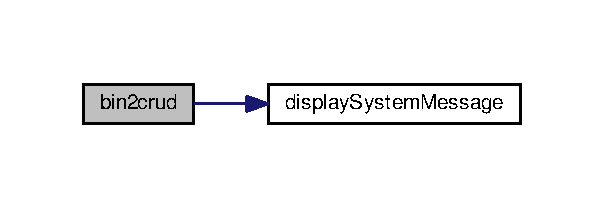
\includegraphics[width=290pt]{manage_user_8php_ac4a74e72e3c7731da127516dd1265aae_cgraph}
\end{center}
\end{figure}



\hypertarget{manage_user_form_8php}{}\section{admin/manage\+User\+Form.php File Reference}
\label{manage_user_form_8php}\index{admin/manage\+User\+Form.\+php@{admin/manage\+User\+Form.\+php}}


backend\+: manage user (html form)  




\subsection{Detailed Description}
Bio\+C\+A\+Se Monitor 2.\+1 \begin{DoxyCopyright}{Copyright}
(C) 2013-\/2018 www.\+museumfuernaturkunde.\+berlin 
\end{DoxyCopyright}
\begin{DoxyAuthor}{Author}
\href{mailto:thomas.pfuhl@mfn.berlin}{\tt thomas.\+pfuhl@mfn.\+berlin} based on Version 1.\+4 written by \href{mailto:falko.gloeckler@mfn.berlin}{\tt falko.\+gloeckler@mfn.\+berlin}
\end{DoxyAuthor}
This program is free software\+: you can redistribute it and/or modify it under the terms of the G\+NU General Public License as published by the Free Software Foundation, either version 3 of the License, or (at your option) any later version.

This program is distributed in the hope that it will be useful, but W\+I\+T\+H\+O\+UT A\+NY W\+A\+R\+R\+A\+N\+TY; without even the implied warranty of M\+E\+R\+C\+H\+A\+N\+T\+A\+B\+I\+L\+I\+TY or F\+I\+T\+N\+E\+SS F\+OR A P\+A\+R\+T\+I\+C\+U\+L\+AR P\+U\+R\+P\+O\+SE. See the G\+NU General Public License for more details.

You should have received a copy of the G\+NU General Public License along with this program. If not, see \href{http://www.gnu.org/licenses/}{\tt http\+://www.\+gnu.\+org/licenses/}. 
\hypertarget{admin_2navbar_8php}{}\section{admin/navbar.php File Reference}
\label{admin_2navbar_8php}\index{admin/navbar.\+php@{admin/navbar.\+php}}


backend\+: display navigation bar  


\subsection*{Namespaces}
\begin{DoxyCompactItemize}
\item 
 \hyperlink{namespace_bms}{Bms}
\end{DoxyCompactItemize}


\subsection{Detailed Description}
Bio\+C\+A\+Se Monitor 2.\+1 \begin{DoxyCopyright}{Copyright}
(C) 2013-\/2018 www.\+museumfuernaturkunde.\+berlin 
\end{DoxyCopyright}
\begin{DoxyAuthor}{Author}
\href{mailto:thomas.pfuhl@mfn.berlin}{\tt thomas.\+pfuhl@mfn.\+berlin} based on Version 1.\+4 written by \href{mailto:falko.gloeckler@mfn.berlin}{\tt falko.\+gloeckler@mfn.\+berlin}
\end{DoxyAuthor}
This program is free software\+: you can redistribute it and/or modify it under the terms of the G\+NU General Public License as published by the Free Software Foundation, either version 3 of the License, or (at your option) any later version.

This program is distributed in the hope that it will be useful, but W\+I\+T\+H\+O\+UT A\+NY W\+A\+R\+R\+A\+N\+TY; without even the implied warranty of M\+E\+R\+C\+H\+A\+N\+T\+A\+B\+I\+L\+I\+TY or F\+I\+T\+N\+E\+SS F\+OR A P\+A\+R\+T\+I\+C\+U\+L\+AR P\+U\+R\+P\+O\+SE. See the G\+NU General Public License for more details.

You should have received a copy of the G\+NU General Public License along with this program. If not, see \href{http://www.gnu.org/licenses/}{\tt http\+://www.\+gnu.\+org/licenses/}. 
\hypertarget{consistency_2navbar_8php}{}\section{consistency/navbar.php File Reference}
\label{consistency_2navbar_8php}\index{consistency/navbar.\+php@{consistency/navbar.\+php}}


display bootstrap navigation bar  


\subsection*{Namespaces}
\begin{DoxyCompactItemize}
\item 
 \hyperlink{namespace_consistency}{Consistency}
\end{DoxyCompactItemize}


\subsection{Detailed Description}
This program is free software\+: you can redistribute it and/or modify it under the terms of the G\+NU General Public License as published by the Free Software Foundation, either version 3 of the License, or (at your option) any later version.

This program is distributed in the hope that it will be useful, but W\+I\+T\+H\+O\+UT A\+NY W\+A\+R\+R\+A\+N\+TY; without even the implied warranty of M\+E\+R\+C\+H\+A\+N\+T\+A\+B\+I\+L\+I\+TY or F\+I\+T\+N\+E\+SS F\+OR A P\+A\+R\+T\+I\+C\+U\+L\+AR P\+U\+R\+P\+O\+SE. See the G\+NU General Public License for more details.

You should have received a copy of the G\+NU General Public License along with this program. If not, see \href{http://www.gnu.org/licenses/}{\tt http\+://www.\+gnu.\+org/licenses/}. 
\hypertarget{services_2navbar_8php}{}\section{services/navbar.php File Reference}
\label{services_2navbar_8php}\index{services/navbar.\+php@{services/navbar.\+php}}


display navigation bar  


\subsection*{Namespaces}
\begin{DoxyCompactItemize}
\item 
 \hyperlink{namespace_bms}{Bms}
\end{DoxyCompactItemize}


\subsection{Detailed Description}
Bio\+C\+A\+Se Monitor 2.\+1 \begin{DoxyCopyright}{Copyright}
(C) 2013-\/2018 www.\+museumfuernaturkunde.\+berlin 
\end{DoxyCopyright}
\begin{DoxyAuthor}{Author}
\href{mailto:thomas.pfuhl@mfn.berlin}{\tt thomas.\+pfuhl@mfn.\+berlin} based on Version 1.\+4 written by \href{mailto:falko.gloeckler@mfn.berlin}{\tt falko.\+gloeckler@mfn.\+berlin}
\end{DoxyAuthor}
This program is free software\+: you can redistribute it and/or modify it under the terms of the G\+NU General Public License as published by the Free Software Foundation, either version 3 of the License, or (at your option) any later version.

This program is distributed in the hope that it will be useful, but W\+I\+T\+H\+O\+UT A\+NY W\+A\+R\+R\+A\+N\+TY; without even the implied warranty of M\+E\+R\+C\+H\+A\+N\+T\+A\+B\+I\+L\+I\+TY or F\+I\+T\+N\+E\+SS F\+OR A P\+A\+R\+T\+I\+C\+U\+L\+AR P\+U\+R\+P\+O\+SE. See the G\+NU General Public License for more details.

You should have received a copy of the G\+NU General Public License along with this program. If not, see \href{http://www.gnu.org/licenses/}{\tt http\+://www.\+gnu.\+org/licenses/}. 
\hypertarget{remove_archive_8php}{}\section{admin/remove\+Archive.php File Reference}
\label{remove_archive_8php}\index{admin/remove\+Archive.\+php@{admin/remove\+Archive.\+php}}


backend\+: remove an Archive  




\subsection{Detailed Description}
Bio\+C\+A\+Se Monitor 2.\+1 \begin{DoxyCopyright}{Copyright}
(C) 2013-\/2018 www.\+museumfuernaturkunde.\+berlin 
\end{DoxyCopyright}
\begin{DoxyAuthor}{Author}
\href{mailto:thomas.pfuhl@mfn.berlin}{\tt thomas.\+pfuhl@mfn.\+berlin} based on Version 1.\+4 written by \href{mailto:falko.gloeckler@mfn.berlin}{\tt falko.\+gloeckler@mfn.\+berlin}
\end{DoxyAuthor}
This program is free software\+: you can redistribute it and/or modify it under the terms of the G\+NU General Public License as published by the Free Software Foundation, either version 3 of the License, or (at your option) any later version.

This program is distributed in the hope that it will be useful, but W\+I\+T\+H\+O\+UT A\+NY W\+A\+R\+R\+A\+N\+TY; without even the implied warranty of M\+E\+R\+C\+H\+A\+N\+T\+A\+B\+I\+L\+I\+TY or F\+I\+T\+N\+E\+SS F\+OR A P\+A\+R\+T\+I\+C\+U\+L\+AR P\+U\+R\+P\+O\+SE. See the G\+NU General Public License for more details.

You should have received a copy of the G\+NU General Public License along with this program. If not, see \href{http://www.gnu.org/licenses/}{\tt http\+://www.\+gnu.\+org/licenses/}. 
\hypertarget{remove_count_8php}{}\section{admin/remove\+Count.php File Reference}
\label{remove_count_8php}\index{admin/remove\+Count.\+php@{admin/remove\+Count.\+php}}


backend\+: remove a Count Concept  




\subsection{Detailed Description}
Bio\+C\+A\+Se Monitor 2.\+1 \begin{DoxyCopyright}{Copyright}
(C) 2013-\/2018 www.\+museumfuernaturkunde.\+berlin 
\end{DoxyCopyright}
\begin{DoxyAuthor}{Author}
\href{mailto:thomas.pfuhl@mfn.berlin}{\tt thomas.\+pfuhl@mfn.\+berlin} based on Version 1.\+4 written by \href{mailto:falko.gloeckler@mfn.berlin}{\tt falko.\+gloeckler@mfn.\+berlin}
\end{DoxyAuthor}
This program is free software\+: you can redistribute it and/or modify it under the terms of the G\+NU General Public License as published by the Free Software Foundation, either version 3 of the License, or (at your option) any later version.

This program is distributed in the hope that it will be useful, but W\+I\+T\+H\+O\+UT A\+NY W\+A\+R\+R\+A\+N\+TY; without even the implied warranty of M\+E\+R\+C\+H\+A\+N\+T\+A\+B\+I\+L\+I\+TY or F\+I\+T\+N\+E\+SS F\+OR A P\+A\+R\+T\+I\+C\+U\+L\+AR P\+U\+R\+P\+O\+SE. See the G\+NU General Public License for more details.

You should have received a copy of the G\+NU General Public License along with this program. If not, see \href{http://www.gnu.org/licenses/}{\tt http\+://www.\+gnu.\+org/licenses/}. 
\hypertarget{remove_d_s_a_8php}{}\section{admin/remove\+D\+SA.php File Reference}
\label{remove_d_s_a_8php}\index{admin/remove\+D\+S\+A.\+php@{admin/remove\+D\+S\+A.\+php}}


backend\+: remove a Data Access Point  




\subsection{Detailed Description}
Bio\+C\+A\+Se Monitor 2.\+1 \begin{DoxyCopyright}{Copyright}
(C) 2013-\/2018 www.\+museumfuernaturkunde.\+berlin 
\end{DoxyCopyright}
\begin{DoxyAuthor}{Author}
\href{mailto:thomas.pfuhl@mfn.berlin}{\tt thomas.\+pfuhl@mfn.\+berlin} based on Version 1.\+4 written by \href{mailto:falko.gloeckler@mfn.berlin}{\tt falko.\+gloeckler@mfn.\+berlin}
\end{DoxyAuthor}
This program is free software\+: you can redistribute it and/or modify it under the terms of the G\+NU General Public License as published by the Free Software Foundation, either version 3 of the License, or (at your option) any later version.

This program is distributed in the hope that it will be useful, but W\+I\+T\+H\+O\+UT A\+NY W\+A\+R\+R\+A\+N\+TY; without even the implied warranty of M\+E\+R\+C\+H\+A\+N\+T\+A\+B\+I\+L\+I\+TY or F\+I\+T\+N\+E\+SS F\+OR A P\+A\+R\+T\+I\+C\+U\+L\+AR P\+U\+R\+P\+O\+SE. See the G\+NU General Public License for more details.

You should have received a copy of the G\+NU General Public License along with this program. If not, see \href{http://www.gnu.org/licenses/}{\tt http\+://www.\+gnu.\+org/licenses/}. 
\hypertarget{remove_useful_link_8php}{}\section{admin/remove\+Useful\+Link.php File Reference}
\label{remove_useful_link_8php}\index{admin/remove\+Useful\+Link.\+php@{admin/remove\+Useful\+Link.\+php}}


backend\+: remove a useful Link  




\subsection{Detailed Description}
Bio\+C\+A\+Se Monitor 2.\+1 \begin{DoxyCopyright}{Copyright}
(C) 2013-\/2018 www.\+museumfuernaturkunde.\+berlin 
\end{DoxyCopyright}
\begin{DoxyAuthor}{Author}
\href{mailto:thomas.pfuhl@mfn.berlin}{\tt thomas.\+pfuhl@mfn.\+berlin} based on Version 1.\+4 written by \href{mailto:falko.gloeckler@mfn.berlin}{\tt falko.\+gloeckler@mfn.\+berlin}
\end{DoxyAuthor}
This program is free software\+: you can redistribute it and/or modify it under the terms of the G\+NU General Public License as published by the Free Software Foundation, either version 3 of the License, or (at your option) any later version.

This program is distributed in the hope that it will be useful, but W\+I\+T\+H\+O\+UT A\+NY W\+A\+R\+R\+A\+N\+TY; without even the implied warranty of M\+E\+R\+C\+H\+A\+N\+T\+A\+B\+I\+L\+I\+TY or F\+I\+T\+N\+E\+SS F\+OR A P\+A\+R\+T\+I\+C\+U\+L\+AR P\+U\+R\+P\+O\+SE. See the G\+NU General Public License for more details.

You should have received a copy of the G\+NU General Public License along with this program. If not, see \href{http://www.gnu.org/licenses/}{\tt http\+://www.\+gnu.\+org/licenses/}. 
\hypertarget{sort_archives_8php}{}\section{admin/sort\+Archives.php File Reference}
\label{sort_archives_8php}\index{admin/sort\+Archives.\+php@{admin/sort\+Archives.\+php}}


backend\+: sort Bio\+C\+A\+Se X\+ML Archives  




\subsection{Detailed Description}
Bio\+C\+A\+Se Monitor 2.\+1 \begin{DoxyCopyright}{Copyright}
(C) 2013-\/2018 www.\+museumfuernaturkunde.\+berlin 
\end{DoxyCopyright}
\begin{DoxyAuthor}{Author}
\href{mailto:thomas.pfuhl@mfn.berlin}{\tt thomas.\+pfuhl@mfn.\+berlin} based on Version 1.\+4 written by \href{mailto:falko.gloeckler@mfn.berlin}{\tt falko.\+gloeckler@mfn.\+berlin}
\end{DoxyAuthor}
This program is free software\+: you can redistribute it and/or modify it under the terms of the G\+NU General Public License as published by the Free Software Foundation, either version 3 of the License, or (at your option) any later version.

This program is distributed in the hope that it will be useful, but W\+I\+T\+H\+O\+UT A\+NY W\+A\+R\+R\+A\+N\+TY; without even the implied warranty of M\+E\+R\+C\+H\+A\+N\+T\+A\+B\+I\+L\+I\+TY or F\+I\+T\+N\+E\+SS F\+OR A P\+A\+R\+T\+I\+C\+U\+L\+AR P\+U\+R\+P\+O\+SE. See the G\+NU General Public License for more details.

You should have received a copy of the G\+NU General Public License along with this program. If not, see \href{http://www.gnu.org/licenses/}{\tt http\+://www.\+gnu.\+org/licenses/}. 
\hypertarget{sort_count_concepts_8php}{}\section{admin/sort\+Count\+Concepts.php File Reference}
\label{sort_count_concepts_8php}\index{admin/sort\+Count\+Concepts.\+php@{admin/sort\+Count\+Concepts.\+php}}


backend\+: sort Count Concepts  




\subsection{Detailed Description}
Bio\+C\+A\+Se Monitor 2.\+1 \begin{DoxyCopyright}{Copyright}
(C) 2013-\/2018 www.\+museumfuernaturkunde.\+berlin 
\end{DoxyCopyright}
\begin{DoxyAuthor}{Author}
\href{mailto:thomas.pfuhl@mfn.berlin}{\tt thomas.\+pfuhl@mfn.\+berlin} based on Version 1.\+4 written by \href{mailto:falko.gloeckler@mfn.berlin}{\tt falko.\+gloeckler@mfn.\+berlin}
\end{DoxyAuthor}
This program is free software\+: you can redistribute it and/or modify it under the terms of the G\+NU General Public License as published by the Free Software Foundation, either version 3 of the License, or (at your option) any later version.

This program is distributed in the hope that it will be useful, but W\+I\+T\+H\+O\+UT A\+NY W\+A\+R\+R\+A\+N\+TY; without even the implied warranty of M\+E\+R\+C\+H\+A\+N\+T\+A\+B\+I\+L\+I\+TY or F\+I\+T\+N\+E\+SS F\+OR A P\+A\+R\+T\+I\+C\+U\+L\+AR P\+U\+R\+P\+O\+SE. See the G\+NU General Public License for more details.

You should have received a copy of the G\+NU General Public License along with this program. If not, see \href{http://www.gnu.org/licenses/}{\tt http\+://www.\+gnu.\+org/licenses/}. 
\hypertarget{sort_useful_links_8php}{}\section{admin/sort\+Useful\+Links.php File Reference}
\label{sort_useful_links_8php}\index{admin/sort\+Useful\+Links.\+php@{admin/sort\+Useful\+Links.\+php}}


backend\+: sort Useful Links  




\subsection{Detailed Description}
Bio\+C\+A\+Se Monitor 2.\+1 \begin{DoxyCopyright}{Copyright}
(C) 2013-\/2018 www.\+museumfuernaturkunde.\+berlin 
\end{DoxyCopyright}
\begin{DoxyAuthor}{Author}
\href{mailto:thomas.pfuhl@mfn.berlin}{\tt thomas.\+pfuhl@mfn.\+berlin} based on Version 1.\+4 written by \href{mailto:falko.gloeckler@mfn.berlin}{\tt falko.\+gloeckler@mfn.\+berlin}
\end{DoxyAuthor}
This program is free software\+: you can redistribute it and/or modify it under the terms of the G\+NU General Public License as published by the Free Software Foundation, either version 3 of the License, or (at your option) any later version.

This program is distributed in the hope that it will be useful, but W\+I\+T\+H\+O\+UT A\+NY W\+A\+R\+R\+A\+N\+TY; without even the implied warranty of M\+E\+R\+C\+H\+A\+N\+T\+A\+B\+I\+L\+I\+TY or F\+I\+T\+N\+E\+SS F\+OR A P\+A\+R\+T\+I\+C\+U\+L\+AR P\+U\+R\+P\+O\+SE. See the G\+NU General Public License for more details.

You should have received a copy of the G\+NU General Public License along with this program. If not, see \href{http://www.gnu.org/licenses/}{\tt http\+://www.\+gnu.\+org/licenses/}. 
\hypertarget{update_archive_8php}{}\section{admin/update\+Archive.php File Reference}
\label{update_archive_8php}\index{admin/update\+Archive.\+php@{admin/update\+Archive.\+php}}


backend\+: update X\+ML Archive  




\subsection{Detailed Description}
Bio\+C\+A\+Se Monitor 2.\+1 \begin{DoxyCopyright}{Copyright}
(C) 2013-\/2018 www.\+museumfuernaturkunde.\+berlin 
\end{DoxyCopyright}
\begin{DoxyAuthor}{Author}
\href{mailto:thomas.pfuhl@mfn.berlin}{\tt thomas.\+pfuhl@mfn.\+berlin} based on Version 1.\+4 written by \href{mailto:falko.gloeckler@mfn.berlin}{\tt falko.\+gloeckler@mfn.\+berlin}
\end{DoxyAuthor}
This program is free software\+: you can redistribute it and/or modify it under the terms of the G\+NU General Public License as published by the Free Software Foundation, either version 3 of the License, or (at your option) any later version.

This program is distributed in the hope that it will be useful, but W\+I\+T\+H\+O\+UT A\+NY W\+A\+R\+R\+A\+N\+TY; without even the implied warranty of M\+E\+R\+C\+H\+A\+N\+T\+A\+B\+I\+L\+I\+TY or F\+I\+T\+N\+E\+SS F\+OR A P\+A\+R\+T\+I\+C\+U\+L\+AR P\+U\+R\+P\+O\+SE. See the G\+NU General Public License for more details.

You should have received a copy of the G\+NU General Public License along with this program. If not, see \href{http://www.gnu.org/licenses/}{\tt http\+://www.\+gnu.\+org/licenses/}. 
\hypertarget{update_count_concept_8php}{}\section{admin/update\+Count\+Concept.php File Reference}
\label{update_count_concept_8php}\index{admin/update\+Count\+Concept.\+php@{admin/update\+Count\+Concept.\+php}}


backend\+: update Count Concept  




\subsection{Detailed Description}
Bio\+C\+A\+Se Monitor 2.\+1 \begin{DoxyCopyright}{Copyright}
(C) 2013-\/2018 www.\+museumfuernaturkunde.\+berlin 
\end{DoxyCopyright}
\begin{DoxyAuthor}{Author}
\href{mailto:thomas.pfuhl@mfn.berlin}{\tt thomas.\+pfuhl@mfn.\+berlin} based on Version 1.\+4 written by \href{mailto:falko.gloeckler@mfn.berlin}{\tt falko.\+gloeckler@mfn.\+berlin}
\end{DoxyAuthor}
This program is free software\+: you can redistribute it and/or modify it under the terms of the G\+NU General Public License as published by the Free Software Foundation, either version 3 of the License, or (at your option) any later version.

This program is distributed in the hope that it will be useful, but W\+I\+T\+H\+O\+UT A\+NY W\+A\+R\+R\+A\+N\+TY; without even the implied warranty of M\+E\+R\+C\+H\+A\+N\+T\+A\+B\+I\+L\+I\+TY or F\+I\+T\+N\+E\+SS F\+OR A P\+A\+R\+T\+I\+C\+U\+L\+AR P\+U\+R\+P\+O\+SE. See the G\+NU General Public License for more details.

You should have received a copy of the G\+NU General Public License along with this program. If not, see \href{http://www.gnu.org/licenses/}{\tt http\+://www.\+gnu.\+org/licenses/}. 
\hypertarget{update_d_s_a_8php}{}\section{admin/update\+D\+SA.php File Reference}
\label{update_d_s_a_8php}\index{admin/update\+D\+S\+A.\+php@{admin/update\+D\+S\+A.\+php}}


backend\+: update Data Source Access Point  




\subsection{Detailed Description}
Bio\+C\+A\+Se Monitor 2.\+1 \begin{DoxyCopyright}{Copyright}
(C) 2013-\/2018 www.\+museumfuernaturkunde.\+berlin 
\end{DoxyCopyright}
\begin{DoxyAuthor}{Author}
\href{mailto:thomas.pfuhl@mfn.berlin}{\tt thomas.\+pfuhl@mfn.\+berlin} based on Version 1.\+4 written by \href{mailto:falko.gloeckler@mfn.berlin}{\tt falko.\+gloeckler@mfn.\+berlin}
\end{DoxyAuthor}
This program is free software\+: you can redistribute it and/or modify it under the terms of the G\+NU General Public License as published by the Free Software Foundation, either version 3 of the License, or (at your option) any later version.

This program is distributed in the hope that it will be useful, but W\+I\+T\+H\+O\+UT A\+NY W\+A\+R\+R\+A\+N\+TY; without even the implied warranty of M\+E\+R\+C\+H\+A\+N\+T\+A\+B\+I\+L\+I\+TY or F\+I\+T\+N\+E\+SS F\+OR A P\+A\+R\+T\+I\+C\+U\+L\+AR P\+U\+R\+P\+O\+SE. See the G\+NU General Public License for more details.

You should have received a copy of the G\+NU General Public License along with this program. If not, see \href{http://www.gnu.org/licenses/}{\tt http\+://www.\+gnu.\+org/licenses/}. 
\hypertarget{update_main_metadata_8php}{}\section{admin/update\+Main\+Metadata.php File Reference}
\label{update_main_metadata_8php}\index{admin/update\+Main\+Metadata.\+php@{admin/update\+Main\+Metadata.\+php}}


backend\+: update main metedata for a given provider  




\subsection{Detailed Description}
Bio\+C\+A\+Se Monitor 2.\+1 \begin{DoxyCopyright}{Copyright}
(C) 2013-\/2018 www.\+museumfuernaturkunde.\+berlin 
\end{DoxyCopyright}
\begin{DoxyAuthor}{Author}
\href{mailto:thomas.pfuhl@mfn.berlin}{\tt thomas.\+pfuhl@mfn.\+berlin} based on Version 1.\+4 written by \href{mailto:falko.gloeckler@mfn.berlin}{\tt falko.\+gloeckler@mfn.\+berlin}
\end{DoxyAuthor}
This program is free software\+: you can redistribute it and/or modify it under the terms of the G\+NU General Public License as published by the Free Software Foundation, either version 3 of the License, or (at your option) any later version.

This program is distributed in the hope that it will be useful, but W\+I\+T\+H\+O\+UT A\+NY W\+A\+R\+R\+A\+N\+TY; without even the implied warranty of M\+E\+R\+C\+H\+A\+N\+T\+A\+B\+I\+L\+I\+TY or F\+I\+T\+N\+E\+SS F\+OR A P\+A\+R\+T\+I\+C\+U\+L\+AR P\+U\+R\+P\+O\+SE. See the G\+NU General Public License for more details.

You should have received a copy of the G\+NU General Public License along with this program. If not, see \href{http://www.gnu.org/licenses/}{\tt http\+://www.\+gnu.\+org/licenses/}. 
\hypertarget{update_useful_link_8php}{}\section{admin/update\+Useful\+Link.php File Reference}
\label{update_useful_link_8php}\index{admin/update\+Useful\+Link.\+php@{admin/update\+Useful\+Link.\+php}}


backend\+: update useful link  




\subsection{Detailed Description}
Bio\+C\+A\+Se Monitor 2.\+1 \begin{DoxyCopyright}{Copyright}
(C) 2013-\/2018 www.\+museumfuernaturkunde.\+berlin 
\end{DoxyCopyright}
\begin{DoxyAuthor}{Author}
\href{mailto:thomas.pfuhl@mfn.berlin}{\tt thomas.\+pfuhl@mfn.\+berlin} based on Version 1.\+4 written by \href{mailto:falko.gloeckler@mfn.berlin}{\tt falko.\+gloeckler@mfn.\+berlin}
\end{DoxyAuthor}
This program is free software\+: you can redistribute it and/or modify it under the terms of the G\+NU General Public License as published by the Free Software Foundation, either version 3 of the License, or (at your option) any later version.

This program is distributed in the hope that it will be useful, but W\+I\+T\+H\+O\+UT A\+NY W\+A\+R\+R\+A\+N\+TY; without even the implied warranty of M\+E\+R\+C\+H\+A\+N\+T\+A\+B\+I\+L\+I\+TY or F\+I\+T\+N\+E\+SS F\+OR A P\+A\+R\+T\+I\+C\+U\+L\+AR P\+U\+R\+P\+O\+SE. See the G\+NU General Public License for more details.

You should have received a copy of the G\+NU General Public License along with this program. If not, see \href{http://www.gnu.org/licenses/}{\tt http\+://www.\+gnu.\+org/licenses/}. 
\hypertarget{config_8sample_8php}{}\section{config/config.sample.\+php File Reference}
\label{config_8sample_8php}\index{config/config.\+sample.\+php@{config/config.\+sample.\+php}}


configuration\+: constants and DB settings  


\subsection*{Namespaces}
\begin{DoxyCompactItemize}
\item 
 \hyperlink{namespace_bms}{Bms}
\end{DoxyCompactItemize}
\subsection*{Functions}
\begin{DoxyCompactItemize}
\item 
\hyperlink{namespace_bms_a72bf47280fcd5e7b7521cecc39ffe509}{init} ()
\end{DoxyCompactItemize}
\subsection*{Variables}
\begin{DoxyCompactItemize}
\item 
const \hyperlink{namespace_bms_a28e24c389e469e22acd9d33abfe3fb4d}{D\+A\+T\+A\+C\+E\+N\+T\+E\+R\+\_\+\+N\+A\+ME} \char`\"{}Data Center \char`\"{}
\item 
const \hyperlink{namespace_bms_a6d448b74f10f8080293b329a47a046b4}{S\+A\+LT} \char`\"{}WE@leht-\/=13\char`\"{}
\item 
const \hyperlink{namespace_bms_af070310b6692d4e96af677af14648411}{V\+E\+R\+B\+O\+SE} 3
\item 
const \hyperlink{namespace_bms_a7af7ef3e15183adae80bfc7cf0272937}{D\+E\+B\+U\+G\+M\+O\+DE} 1
\item 
const \hyperlink{namespace_bms_a4b14ca0fbcdfa3f37da752304008a9c1}{C\+U\+S\+T\+OM} 1
\item 
const \hyperlink{namespace_bms_ac3ff4673172a882fa4a11351118e2716}{C\+A\+C\+H\+I\+N\+G\+\_\+\+I\+N\+T\+E\+R\+V\+AL} 604800
\item 
const \hyperlink{namespace_bms_a43e84be6597c73c02e67db0dc944cd1a}{C\+A\+C\+H\+E\+\_\+\+D\+I\+R\+E\+C\+T\+O\+RY} \char`\"{}data\+\_\+cache/\char`\"{}
\item 
const \hyperlink{namespace_bms_a83815bb64763ef7810008cfe96d0ecf7}{P\+R\+O\+X\+Y\+\_\+\+W\+O\+R\+K\+A\+R\+O\+U\+ND} false
\item 
const \hyperlink{namespace_bms_a796fca3489760c39de0d4efdd11c67de}{P\+R\+O\+X\+Y\+\_\+\+W\+O\+R\+K\+A\+R\+O\+U\+N\+D\+\_\+\+U\+RL} \char`\"{}http\+://192.\+168.\+101.\+160/biocasemonitor/gfbio\char`\"{}
\item 
const \hyperlink{namespace_bms_a525a6614ba9af7ba1f60bb7e60572a0c}{D\+B\+\_\+\+D\+IR} \char`\"{}/path/to/db/folder\char`\"{}
\item 
const \hyperlink{namespace_bms_abc05b2c0a077204fb0ef0f345a8f006f}{D\+B\+\_\+\+F\+I\+L\+E\+N\+A\+ME} \char`\"{}provider.\+sqlite\char`\"{}
\item 
\hyperlink{namespace_bms_a1fa3127fc82f96b1436d871ef02be319}{\$db} = null
\item 
const \hyperlink{namespace_bms_ad080a43f212802d39f67f19feeb26dfe}{T\+O\+T\+AL} (!defined(\char`\"{}J\+S\+O\+N\+\_\+\+P\+R\+E\+T\+T\+Y\+\_\+\+P\+R\+I\+NT\char`\"{})) 1
\item 
const \hyperlink{namespace_bms_a99cb80c249c1d51aa36375cca5921896}{D\+I\+S\+T\+I\+N\+CT} 2
\item 
const \hyperlink{namespace_bms_ac8aa145c99391c64083d1ab9451eedef}{D\+R\+O\+P\+P\+ED} 4
\end{DoxyCompactItemize}


\subsection{Detailed Description}
Bio\+C\+A\+Se Monitor 2.\+1 \begin{DoxyCopyright}{Copyright}
(C) 2013-\/2018 www.\+museumfuernaturkunde.\+berlin 
\end{DoxyCopyright}
\begin{DoxyAuthor}{Author}
\href{mailto:thomas.pfuhl@mfn.berlin}{\tt thomas.\+pfuhl@mfn.\+berlin} based on Version 1.\+4 written by \href{mailto:falko.gloeckler@mfn.berlin}{\tt falko.\+gloeckler@mfn.\+berlin}
\end{DoxyAuthor}
This program is free software\+: you can redistribute it and/or modify it under the terms of the G\+NU General Public License as published by the Free Software Foundation, either version 3 of the License, or (at your option) any later version.

This program is distributed in the hope that it will be useful, but W\+I\+T\+H\+O\+UT A\+NY W\+A\+R\+R\+A\+N\+TY; without even the implied warranty of M\+E\+R\+C\+H\+A\+N\+T\+A\+B\+I\+L\+I\+TY or F\+I\+T\+N\+E\+SS F\+OR A P\+A\+R\+T\+I\+C\+U\+L\+AR P\+U\+R\+P\+O\+SE. See the G\+NU General Public License for more details.

You should have received a copy of the G\+NU General Public License along with this program. If not, see \href{http://www.gnu.org/licenses/}{\tt http\+://www.\+gnu.\+org/licenses/}. 
\hypertarget{customize_8php}{}\section{config/custom/customize.php File Reference}
\label{customize_8php}\index{config/custom/customize.\+php@{config/custom/customize.\+php}}


customization  


\subsection*{Namespaces}
\begin{DoxyCompactItemize}
\item 
 \hyperlink{namespace_bms}{Bms}
\end{DoxyCompactItemize}


\subsection{Detailed Description}
This program is free software\+: you can redistribute it and/or modify it under the terms of the G\+NU General Public License as published by the Free Software Foundation, either version 3 of the License, or (at your option) any later version.

This program is distributed in the hope that it will be useful, but W\+I\+T\+H\+O\+UT A\+NY W\+A\+R\+R\+A\+N\+TY; without even the implied warranty of M\+E\+R\+C\+H\+A\+N\+T\+A\+B\+I\+L\+I\+TY or F\+I\+T\+N\+E\+SS F\+OR A P\+A\+R\+T\+I\+C\+U\+L\+AR P\+U\+R\+P\+O\+SE. See the G\+NU General Public License for more details.

You should have received a copy of the G\+NU General Public License along with this program. If not, see \href{http://www.gnu.org/licenses/}{\tt http\+://www.\+gnu.\+org/licenses/}. 
\hypertarget{cardinal_concept_8php}{}\section{consistency/cardinal\+Concept.php File Reference}
\label{cardinal_concept_8php}\index{consistency/cardinal\+Concept.\+php@{consistency/cardinal\+Concept.\+php}}


count the occurrences of given concept  


\subsection*{Namespaces}
\begin{DoxyCompactItemize}
\item 
 \hyperlink{namespace_consistency}{Consistency}
\end{DoxyCompactItemize}
\subsection*{Functions}
\begin{DoxyCompactItemize}
\item 
\hyperlink{namespace_consistency_ab1a6caf75ca08c5daec473d54c0416da}{get\+\_\+tag} (\$tag, \$xml)
\end{DoxyCompactItemize}
\subsection*{Variables}
\begin{DoxyCompactItemize}
\item 
\hyperlink{namespace_consistency_aac53bdb48bdd96ff9c20e2a86f48ce5f}{\$filter} = filter\+\_\+input(I\+N\+P\+U\+T\+\_\+\+G\+ET, \textquotesingle{}filter\textquotesingle{})
\end{DoxyCompactItemize}


\subsection{Detailed Description}
\$concept is dependant from provider \$specifier\+: T\+O\+T\+A\+L$\vert$\+D\+I\+S\+T\+I\+N\+C\+T$\vert$\+D\+R\+O\+P\+P\+ED = bitmap 1$\vert$2$\vert$4 \$filter is dependant from D\+SA, and dependant from \$specifier

returns J\+S\+ON

This program is free software\+: you can redistribute it and/or modify it under the terms of the G\+NU General Public License as published by the Free Software Foundation, either version 3 of the License, or (at your option) any later version.

This program is distributed in the hope that it will be useful, but W\+I\+T\+H\+O\+UT A\+NY W\+A\+R\+R\+A\+N\+TY; without even the implied warranty of M\+E\+R\+C\+H\+A\+N\+T\+A\+B\+I\+L\+I\+TY or F\+I\+T\+N\+E\+SS F\+OR A P\+A\+R\+T\+I\+C\+U\+L\+AR P\+U\+R\+P\+O\+SE. See the G\+NU General Public License for more details.

You should have received a copy of the G\+NU General Public License along with this program. If not, see \href{http://www.gnu.org/licenses/}{\tt http\+://www.\+gnu.\+org/licenses/}. 
\hypertarget{check_for_errors_8php}{}\section{consistency/check\+For\+Errors.php File Reference}
\label{check_for_errors_8php}\index{consistency/check\+For\+Errors.\+php@{consistency/check\+For\+Errors.\+php}}


checks errors for given concept in the consistency check output  


\subsection*{Namespaces}
\begin{DoxyCompactItemize}
\item 
 \hyperlink{namespace_consistency}{Consistency}
\end{DoxyCompactItemize}
\subsection*{Functions}
\begin{DoxyCompactItemize}
\item 
\hyperlink{namespace_consistency_a4359f5b054e4c15acb39a611e29e17c8}{get\+Schema\+Info} (\$schema)
\item 
\hyperlink{namespace_consistency_a1e0e4ba06ca24d6cd0bda99a99ce9f5d}{get\+Rule\+Info} (\$concept, \$mapping)
\end{DoxyCompactItemize}
\subsection*{Variables}
\begin{DoxyCompactItemize}
\item 
\hyperlink{namespace_consistency_a2c93d0b89d7eadb6b8dfb7c83bc991f9}{\$mapping} = \$\+\_\+\+R\+E\+Q\+U\+E\+ST\mbox{[}\char`\"{}mapping\char`\"{}\mbox{]}
\end{DoxyCompactItemize}


\subsection{Detailed Description}
\begin{DoxyRefDesc}{Todo}
\item[\hyperlink{todo__todo000002}{Todo}]classify rules depending on the weight\end{DoxyRefDesc}


This program is free software\+: you can redistribute it and/or modify it under the terms of the G\+NU General Public License as published by the Free Software Foundation, either version 3 of the License, or (at your option) any later version.

This program is distributed in the hope that it will be useful, but W\+I\+T\+H\+O\+UT A\+NY W\+A\+R\+R\+A\+N\+TY; without even the implied warranty of M\+E\+R\+C\+H\+A\+N\+T\+A\+B\+I\+L\+I\+TY or F\+I\+T\+N\+E\+SS F\+OR A P\+A\+R\+T\+I\+C\+U\+L\+AR P\+U\+R\+P\+O\+SE. See the G\+NU General Public License for more details.

You should have received a copy of the G\+NU General Public License along with this program. If not, see \href{http://www.gnu.org/licenses/}{\tt http\+://www.\+gnu.\+org/licenses/}. 
\hypertarget{check_rules_8php}{}\section{consistency/check\+Rules.php File Reference}
\label{check_rules_8php}\index{consistency/check\+Rules.\+php@{consistency/check\+Rules.\+php}}


get rules from DB table rule, get capabilities from B\+PS via C\+U\+RL, check the rules  


\subsection*{Namespaces}
\begin{DoxyCompactItemize}
\item 
 \hyperlink{namespace_consistency}{Consistency}
\end{DoxyCompactItemize}
\subsection*{Functions}
\begin{DoxyCompactItemize}
\item 
\hyperlink{namespace_consistency_ac3ce77dc252c4606ec6b0378f5d79ac7}{get\+Schemas} ()
\item 
\hyperlink{namespace_consistency_a9bf0ee2da6d3a74ee9dbfcf73ae9842e}{get\+Schema\+Mapping\+Info} (\$mapping)
\item 
\hyperlink{namespace_consistency_a2be2339d3806b3febbdb87bd1c27e603}{get\+Mapped\+Elements\+Without\+Rules} (\$mapping)
\item 
\hyperlink{namespace_consistency_a489e7863dc1879d02c46deb03793bc03}{get\+Mapped\+Elements} (\$mapping)
\end{DoxyCompactItemize}
\subsection*{Variables}
\begin{DoxyCompactItemize}
\item 
\hyperlink{namespace_consistency_aca6ad28ee812df74bbd827a9d244055e}{\$dsa} = \$\+\_\+\+R\+E\+Q\+U\+E\+ST\mbox{[}\char`\"{}dsa\char`\"{}\mbox{]}
\end{DoxyCompactItemize}


\subsection{Detailed Description}
\begin{DoxyRefDesc}{Todo}
\item[\hyperlink{todo__todo000003}{Todo}]C\+U\+RL request can be time consuming\end{DoxyRefDesc}


This program is free software\+: you can redistribute it and/or modify it under the terms of the G\+NU General Public License as published by the Free Software Foundation, either version 3 of the License, or (at your option) any later version.

This program is distributed in the hope that it will be useful, but W\+I\+T\+H\+O\+UT A\+NY W\+A\+R\+R\+A\+N\+TY; without even the implied warranty of M\+E\+R\+C\+H\+A\+N\+T\+A\+B\+I\+L\+I\+TY or F\+I\+T\+N\+E\+SS F\+OR A P\+A\+R\+T\+I\+C\+U\+L\+AR P\+U\+R\+P\+O\+SE. See the G\+NU General Public License for more details.

You should have received a copy of the G\+NU General Public License along with this program. If not, see \href{http://www.gnu.org/licenses/}{\tt http\+://www.\+gnu.\+org/licenses/}. 
\hypertarget{get_example_values_8php}{}\section{consistency/get\+Example\+Values.php File Reference}
\label{get_example_values_8php}\index{consistency/get\+Example\+Values.\+php@{consistency/get\+Example\+Values.\+php}}


get example values for given concept in the consistency check output  


\subsection*{Namespaces}
\begin{DoxyCompactItemize}
\item 
 \hyperlink{namespace_consistency}{Consistency}
\end{DoxyCompactItemize}
\subsection*{Variables}
\begin{DoxyCompactItemize}
\item 
\hyperlink{namespace_consistency_a7ab539c1f2610226e15527ae9f66d1b4}{\$aconcept} = explode(\char`\"{}/\char`\"{}, \$concept)
\item 
\hyperlink{namespace_consistency_a6de4812dd264c558f2dadf3ae20b1da2}{\$concept\+\_\+xpath} = implode(\char`\"{}/abcd\+:\char`\"{}, \$aconcept)
\end{DoxyCompactItemize}


\subsection{Detailed Description}
\begin{DoxyRefDesc}{Todo}
\item[\hyperlink{todo__todo000004}{Todo}]compute element xpath with correct prefix for given schema\end{DoxyRefDesc}


\begin{DoxyNote}{Note}
Example call\+: ./consistency/get\+Example\+Values.php? url=\href{http://biocase.naturkundemuseum-berlin.de/current/pywrapper.cgi?dsa=EDIT_ATBI}{\tt http\+://biocase.\+naturkundemuseum-\/berlin.\+de/current/pywrapper.\+cgi?dsa=\+E\+D\+I\+T\+\_\+\+A\+T\+BI} \&concept=/\+Data\+Sets/\+Data\+Set/\+Units/\+Unit/\+Multi\+Media\+Objects/\+Multi\+Media\+Object/\+File\+U\+RI \&filter=$<$like path=\char`\"{}/\+Data\+Sets/\+Data\+Set/\+Metadata/\+Description/\+Representation/\+Title\char`\"{}$>$E\+D\+IT -\/ A\+T\+BI in Spreewald (Germany)$<$/like$>$
\end{DoxyNote}
This program is free software\+: you can redistribute it and/or modify it under the terms of the G\+NU General Public License as published by the Free Software Foundation, either version 3 of the License, or (at your option) any later version.

This program is distributed in the hope that it will be useful, but W\+I\+T\+H\+O\+UT A\+NY W\+A\+R\+R\+A\+N\+TY; without even the implied warranty of M\+E\+R\+C\+H\+A\+N\+T\+A\+B\+I\+L\+I\+TY or F\+I\+T\+N\+E\+SS F\+OR A P\+A\+R\+T\+I\+C\+U\+L\+AR P\+U\+R\+P\+O\+SE. See the G\+NU General Public License for more details.

You should have received a copy of the G\+NU General Public License along with this program. If not, see \href{http://www.gnu.org/licenses/}{\tt http\+://www.\+gnu.\+org/licenses/}. 
\hypertarget{get_schema_mappings_8php}{}\section{consistency/get\+Schema\+Mappings.php File Reference}
\label{get_schema_mappings_8php}\index{consistency/get\+Schema\+Mappings.\+php@{consistency/get\+Schema\+Mappings.\+php}}


get schema mappings from DB  


\subsection*{Namespaces}
\begin{DoxyCompactItemize}
\item 
 \hyperlink{namespace_consistency}{Consistency}
\end{DoxyCompactItemize}
\subsection*{Functions}
\begin{DoxyCompactItemize}
\item 
\hyperlink{namespace_consistency_aa98f8a888d842fcaefeca3407c10435c}{get\+Schema\+Mappings} (\$mapping)
\end{DoxyCompactItemize}


\subsection{Detailed Description}
This program is free software\+: you can redistribute it and/or modify it under the terms of the G\+NU General Public License as published by the Free Software Foundation, either version 3 of the License, or (at your option) any later version.

This program is distributed in the hope that it will be useful, but W\+I\+T\+H\+O\+UT A\+NY W\+A\+R\+R\+A\+N\+TY; without even the implied warranty of M\+E\+R\+C\+H\+A\+N\+T\+A\+B\+I\+L\+I\+TY or F\+I\+T\+N\+E\+SS F\+OR A P\+A\+R\+T\+I\+C\+U\+L\+AR P\+U\+R\+P\+O\+SE. See the G\+NU General Public License for more details.

You should have received a copy of the G\+NU General Public License along with this program. If not, see \href{http://www.gnu.org/licenses/}{\tt http\+://www.\+gnu.\+org/licenses/}. 
\hypertarget{backend_8js}{}\section{js/backend.js File Reference}
\label{backend_8js}\index{js/backend.\+js@{js/backend.\+js}}


javascript functions used in the backend  


\subsection*{Namespaces}
\begin{DoxyCompactItemize}
\item 
 \hyperlink{namespace_bms}{Bms}
\end{DoxyCompactItemize}
\subsection*{Functions}
\begin{DoxyCompactItemize}
\item 
function \hyperlink{backend_8js_a6879c4dc7db6793991cd72ab19ca85ea}{get\+Providers} ()
\item 
function \hyperlink{backend_8js_ad8bb15255910bba8451a623c74323537}{save\+Main\+Metadata} ()
\item 
function \hyperlink{backend_8js_a51fe50f57ea6df6fb0bcbd22099962ab}{get\+Schemas} (id\+Provider, id\+D\+SA, dsa, selected\+Value)
\item 
function \hyperlink{backend_8js_a06ed191b32ca45ffc8c3ad30bf6f6cf4}{get\+Data\+Source\+Access\+Points} (id\+Provider, url, id\+D\+SA, selected\+Value, data\+Set)
\item 
function \hyperlink{backend_8js_a82c76ce90ab8a91de559f9b35d0088d7}{get\+Data\+Set\+Titles} (id\+D\+SA, url, dataset)
\item 
function \hyperlink{backend_8js_ab2defb5f9c70cf24da0dca77cadcdd4c}{add\+D\+SA} (id\+Provider)
\item 
function \hyperlink{backend_8js_ab8857c782e0fd01946658e1a47bd295c}{save\+D\+S\+A\+Point} (dsa, reload)
\item 
function \hyperlink{backend_8js_a36b49b10ca5bff2748b29988f1582f34}{remove\+D\+SA} (id)
\item 
function \hyperlink{backend_8js_a771a32402016a259aee9ff74cd879048}{add\+Count} ()
\item 
function \hyperlink{backend_8js_aa19813ae51cc1b506e8543a7cd6a0e42}{remove\+Count} (id)
\item 
function \hyperlink{backend_8js_af64a4f08a169e74e835e8779804d2982}{save\+Count} (id)
\item 
function \hyperlink{backend_8js_ad5ab46bd92d3669ddd8132202861904c}{add\+Archive} (id\+D\+SA, id\+Provider)
\item 
function \hyperlink{backend_8js_a855d7bfb70d494b3a5937f118e0b4e60}{save\+Archive} (id\+Provider, id\+D\+SA, id)
\item 
function \hyperlink{backend_8js_a15d235044db55b8761af5c59ac1673a1}{hide\+Archive} (id\+D\+SA, id, counter)
\item 
function \hyperlink{backend_8js_afb708a6ab2f049a160aa9c65fb61bd75}{show\+Archive} (id\+D\+SA, id)
\item 
function \hyperlink{backend_8js_a67ccb2b34eb0513b50335e24a6b20d40}{remove\+Archive} (id\+D\+SA, id)
\item 
function \hyperlink{backend_8js_a5f2ae9534f84e79f78aaf8a041b0ab57}{add\+Useful\+Link} (id\+D\+SA, id\+Provider)
\item 
function \hyperlink{backend_8js_af3f3dcdc9df4e4491e80cbd1107f6d2d}{show\+Useful\+Link} (id\+D\+SA, id)
\item 
function \hyperlink{backend_8js_a6f43dd08d697f48f45ed08af494d9367}{hide\+Useful\+Link} (id\+D\+SA, id)
\item 
function \hyperlink{backend_8js_a2b6e8bcc79cbc217976969a2c3830205}{remove\+Useful\+Link} (id\+D\+SA, id)
\item 
function \hyperlink{backend_8js_a9980fb97f36014ac0cf30b90df12498b}{save\+Useful\+Link} (id\+Provider, id\+D\+SA, id)
\item 
function \hyperlink{backend_8js_af5cbf7c37f28fddd8b8a5149a7ed5900}{get\+Link\+Categories} ()
\item 
function \hyperlink{backend_8js_a97b71eb0b809c2808e6b79e2503278ba}{delete\+Old\+Values} ()
\item 
function \hyperlink{backend_8js_a46a518d9683fe224cd47219f3da32d07}{get\+Count\+Concepts} (id\+Provider)
\item 
function \hyperlink{backend_8js_abcad65499b560fbefbaa2b51424bf9ff}{get\+Capabilities} (provider, id\+D\+SA, dsa)
\item 
function \hyperlink{backend_8js_a5f8e953a90f434851f20518b1e3baeb6}{get\+Archives} (id\+Provider, id\+D\+SA)
\item 
function \hyperlink{backend_8js_add7d88a4ad05a1fb2478eff9a1857824}{get\+Useful\+Links} (id\+Provider, id\+D\+SA)
\item 
function \hyperlink{backend_8js_a40b1dad19404febd0ef4c2b8be5e1033}{get\+All\+Metadata} (id\+Provider)
\end{DoxyCompactItemize}


\subsection{Detailed Description}
This program is free software\+: you can redistribute it and/or modify it under the terms of the G\+NU General Public License as published by the Free Software Foundation, either version 3 of the License, or (at your option) any later version.

This program is distributed in the hope that it will be useful, but W\+I\+T\+H\+O\+UT A\+NY W\+A\+R\+R\+A\+N\+TY; without even the implied warranty of M\+E\+R\+C\+H\+A\+N\+T\+A\+B\+I\+L\+I\+TY or F\+I\+T\+N\+E\+SS F\+OR A P\+A\+R\+T\+I\+C\+U\+L\+AR P\+U\+R\+P\+O\+SE. See the G\+NU General Public License for more details.

You should have received a copy of the G\+NU General Public License along with this program. If not, see \href{http://www.gnu.org/licenses/}{\tt http\+://www.\+gnu.\+org/licenses/}. 

\subsection{Function Documentation}
\index{backend.\+js@{backend.\+js}!add\+Archive@{add\+Archive}}
\index{add\+Archive@{add\+Archive}!backend.\+js@{backend.\+js}}
\subsubsection[{\texorpdfstring{add\+Archive(id\+D\+S\+A, id\+Provider)}{addArchive(idDSA, idProvider)}}]{\setlength{\rightskip}{0pt plus 5cm}function add\+Archive (
\begin{DoxyParamCaption}
\item[{}]{id\+D\+SA, }
\item[{}]{id\+Provider}
\end{DoxyParamCaption}
)}\hypertarget{backend_8js_ad5ab46bd92d3669ddd8132202861904c}{}\label{backend_8js_ad5ab46bd92d3669ddd8132202861904c}
adds an Archive


\begin{DoxyParams}[1]{Parameters}
int & {\em \$id\+D\+SA} & ID of Data Source Access Point \\
\hline
int & {\em \$id\+Provider} & ID of Data Center \\
\hline
\end{DoxyParams}
\begin{DoxyReturn}{Returns}
void 
\end{DoxyReturn}


Definition at line 809 of file backend.\+js.

\index{backend.\+js@{backend.\+js}!add\+Count@{add\+Count}}
\index{add\+Count@{add\+Count}!backend.\+js@{backend.\+js}}
\subsubsection[{\texorpdfstring{add\+Count()}{addCount()}}]{\setlength{\rightskip}{0pt plus 5cm}function add\+Count (
\begin{DoxyParamCaption}
{}
\end{DoxyParamCaption}
)}\hypertarget{backend_8js_a771a32402016a259aee9ff74cd879048}{}\label{backend_8js_a771a32402016a259aee9ff74cd879048}
adds a Count Concept \begin{DoxyRefDesc}{Todo}
\item[\hyperlink{todo__todo000008}{Todo}]\+: attach count concepts to each D\+SA, since d\+D\+S\+As may have distinct schemas \end{DoxyRefDesc}
\begin{DoxyReturn}{Returns}
void 
\end{DoxyReturn}


Definition at line 687 of file backend.\+js.

\index{backend.\+js@{backend.\+js}!add\+D\+SA@{add\+D\+SA}}
\index{add\+D\+SA@{add\+D\+SA}!backend.\+js@{backend.\+js}}
\subsubsection[{\texorpdfstring{add\+D\+S\+A(id\+Provider)}{addDSA(idProvider)}}]{\setlength{\rightskip}{0pt plus 5cm}function add\+D\+SA (
\begin{DoxyParamCaption}
\item[{}]{id\+Provider}
\end{DoxyParamCaption}
)}\hypertarget{backend_8js_ab2defb5f9c70cf24da0dca77cadcdd4c}{}\label{backend_8js_ab2defb5f9c70cf24da0dca77cadcdd4c}
creates new D\+SA record


\begin{DoxyParams}[1]{Parameters}
int & {\em \$id\+Provider} & \\
\hline
\end{DoxyParams}
\begin{DoxyReturn}{Returns}
boolean false 
\end{DoxyReturn}


Definition at line 284 of file backend.\+js.



Here is the call graph for this function\+:\nopagebreak
\begin{figure}[H]
\begin{center}
\leavevmode
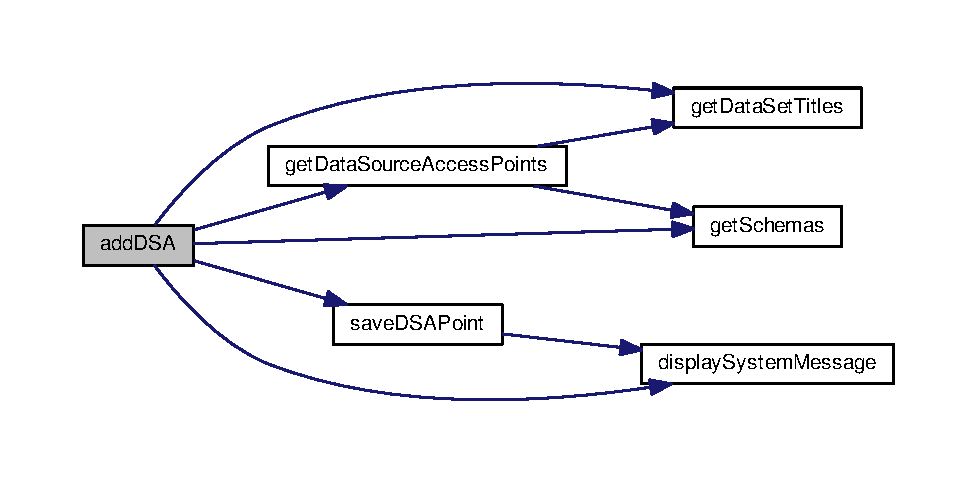
\includegraphics[width=350pt]{backend_8js_ab2defb5f9c70cf24da0dca77cadcdd4c_cgraph}
\end{center}
\end{figure}


\index{backend.\+js@{backend.\+js}!add\+Useful\+Link@{add\+Useful\+Link}}
\index{add\+Useful\+Link@{add\+Useful\+Link}!backend.\+js@{backend.\+js}}
\subsubsection[{\texorpdfstring{add\+Useful\+Link(id\+D\+S\+A, id\+Provider)}{addUsefulLink(idDSA, idProvider)}}]{\setlength{\rightskip}{0pt plus 5cm}function add\+Useful\+Link (
\begin{DoxyParamCaption}
\item[{}]{id\+D\+SA, }
\item[{}]{id\+Provider}
\end{DoxyParamCaption}
)}\hypertarget{backend_8js_a5f2ae9534f84e79f78aaf8a041b0ab57}{}\label{backend_8js_a5f2ae9534f84e79f78aaf8a041b0ab57}
adds a Useful Link


\begin{DoxyParams}[1]{Parameters}
int & {\em \$id\+D\+SA} & ID of Data Source Access Point \\
\hline
int & {\em \$id\+Provider} & ID of Data Center \\
\hline
\end{DoxyParams}
\begin{DoxyReturn}{Returns}
void 
\end{DoxyReturn}


Definition at line 957 of file backend.\+js.

\index{backend.\+js@{backend.\+js}!delete\+Old\+Values@{delete\+Old\+Values}}
\index{delete\+Old\+Values@{delete\+Old\+Values}!backend.\+js@{backend.\+js}}
\subsubsection[{\texorpdfstring{delete\+Old\+Values()}{deleteOldValues()}}]{\setlength{\rightskip}{0pt plus 5cm}function delete\+Old\+Values (
\begin{DoxyParamCaption}
{}
\end{DoxyParamCaption}
)}\hypertarget{backend_8js_a97b71eb0b809c2808e6b79e2503278ba}{}\label{backend_8js_a97b71eb0b809c2808e6b79e2503278ba}
removes displayed infos from the form

\begin{DoxyReturn}{Returns}
boolean false 
\end{DoxyReturn}


Definition at line 1145 of file backend.\+js.



Here is the caller graph for this function\+:\nopagebreak
\begin{figure}[H]
\begin{center}
\leavevmode
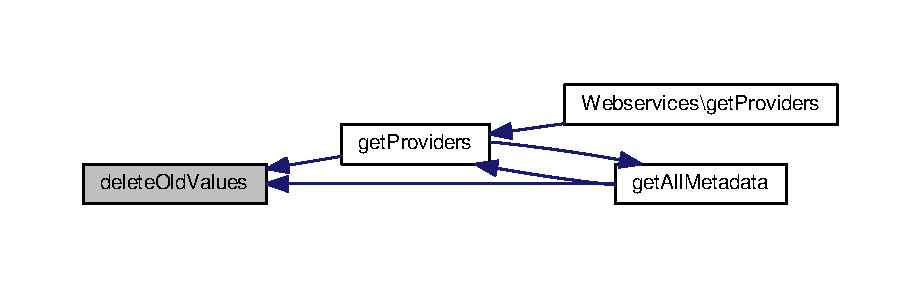
\includegraphics[width=350pt]{backend_8js_a97b71eb0b809c2808e6b79e2503278ba_icgraph}
\end{center}
\end{figure}


\index{backend.\+js@{backend.\+js}!get\+All\+Metadata@{get\+All\+Metadata}}
\index{get\+All\+Metadata@{get\+All\+Metadata}!backend.\+js@{backend.\+js}}
\subsubsection[{\texorpdfstring{get\+All\+Metadata(id\+Provider)}{getAllMetadata(idProvider)}}]{\setlength{\rightskip}{0pt plus 5cm}function get\+All\+Metadata (
\begin{DoxyParamCaption}
\item[{}]{id\+Provider}
\end{DoxyParamCaption}
)}\hypertarget{backend_8js_a40b1dad19404febd0ef4c2b8be5e1033}{}\label{backend_8js_a40b1dad19404febd0ef4c2b8be5e1033}
main function\+: gets all metadata of given provider and populates the html form


\begin{DoxyParams}[1]{Parameters}
int & {\em \$id\+Provider} & \\
\hline
\end{DoxyParams}
\begin{DoxyReturn}{Returns}
boolean false 
\end{DoxyReturn}


Definition at line 1523 of file backend.\+js.



Here is the call graph for this function\+:\nopagebreak
\begin{figure}[H]
\begin{center}
\leavevmode
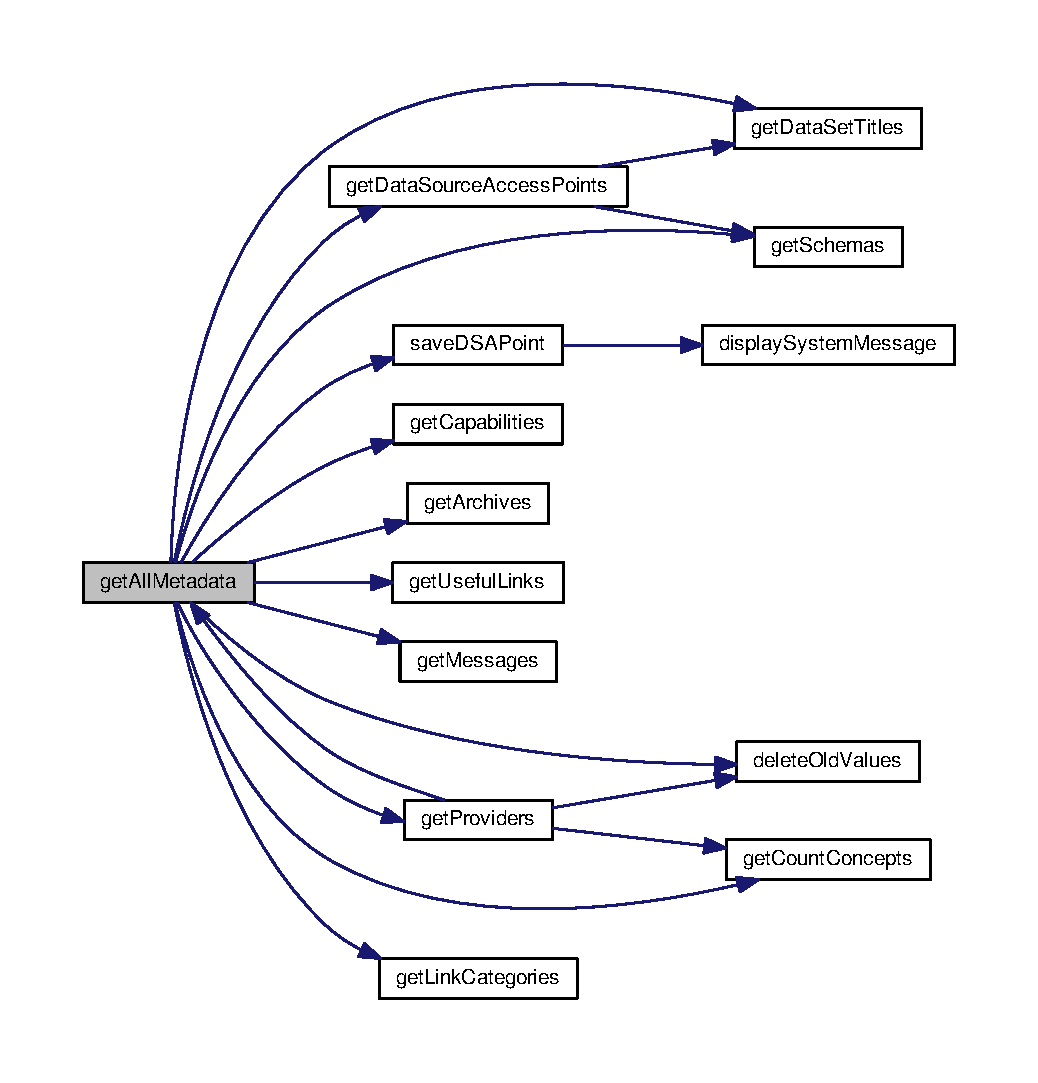
\includegraphics[width=350pt]{backend_8js_a40b1dad19404febd0ef4c2b8be5e1033_cgraph}
\end{center}
\end{figure}




Here is the caller graph for this function\+:\nopagebreak
\begin{figure}[H]
\begin{center}
\leavevmode
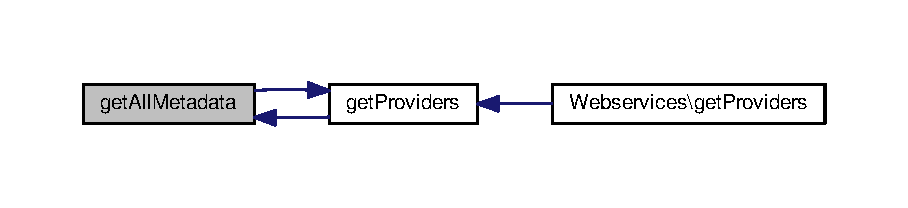
\includegraphics[width=350pt]{backend_8js_a40b1dad19404febd0ef4c2b8be5e1033_icgraph}
\end{center}
\end{figure}


\index{backend.\+js@{backend.\+js}!get\+Archives@{get\+Archives}}
\index{get\+Archives@{get\+Archives}!backend.\+js@{backend.\+js}}
\subsubsection[{\texorpdfstring{get\+Archives(id\+Provider, id\+D\+S\+A)}{getArchives(idProvider, idDSA)}}]{\setlength{\rightskip}{0pt plus 5cm}function get\+Archives (
\begin{DoxyParamCaption}
\item[{}]{id\+Provider, }
\item[{}]{id\+D\+SA}
\end{DoxyParamCaption}
)}\hypertarget{backend_8js_a5f8e953a90f434851f20518b1e3baeb6}{}\label{backend_8js_a5f8e953a90f434851f20518b1e3baeb6}
gets the X\+ML archives for a given D\+SA


\begin{DoxyParams}[1]{Parameters}
int & {\em \$id\+Provider} & \\
\hline
int & {\em \$id\+D\+SA} & \\
\hline
\end{DoxyParams}
\begin{DoxyReturn}{Returns}
boolean false 
\end{DoxyReturn}


Definition at line 1323 of file backend.\+js.



Here is the caller graph for this function\+:\nopagebreak
\begin{figure}[H]
\begin{center}
\leavevmode
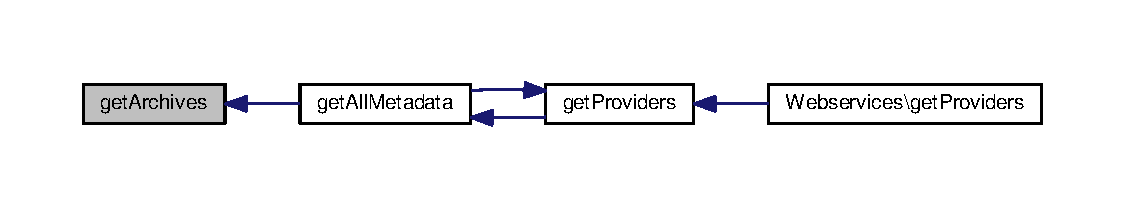
\includegraphics[width=350pt]{backend_8js_a5f8e953a90f434851f20518b1e3baeb6_icgraph}
\end{center}
\end{figure}


\index{backend.\+js@{backend.\+js}!get\+Capabilities@{get\+Capabilities}}
\index{get\+Capabilities@{get\+Capabilities}!backend.\+js@{backend.\+js}}
\subsubsection[{\texorpdfstring{get\+Capabilities(provider, id\+D\+S\+A, dsa)}{getCapabilities(provider, idDSA, dsa)}}]{\setlength{\rightskip}{0pt plus 5cm}function get\+Capabilities (
\begin{DoxyParamCaption}
\item[{}]{provider, }
\item[{}]{id\+D\+SA, }
\item[{}]{dsa}
\end{DoxyParamCaption}
)}\hypertarget{backend_8js_abcad65499b560fbefbaa2b51424bf9ff}{}\label{backend_8js_abcad65499b560fbefbaa2b51424bf9ff}
gets the capabilities


\begin{DoxyParams}[1]{Parameters}
int & {\em \$provider} & \\
\hline
int & {\em \$id\+D\+SA} & \\
\hline
string & {\em \$dsa} & \\
\hline
\end{DoxyParams}
\begin{DoxyReturn}{Returns}
boolean false 
\end{DoxyReturn}


Definition at line 1266 of file backend.\+js.



Here is the caller graph for this function\+:\nopagebreak
\begin{figure}[H]
\begin{center}
\leavevmode
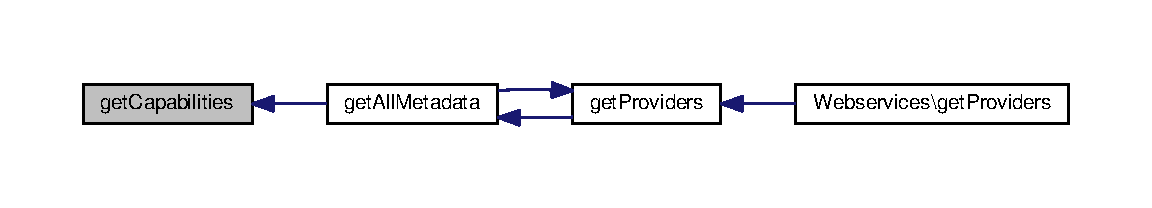
\includegraphics[width=350pt]{backend_8js_abcad65499b560fbefbaa2b51424bf9ff_icgraph}
\end{center}
\end{figure}


\index{backend.\+js@{backend.\+js}!get\+Count\+Concepts@{get\+Count\+Concepts}}
\index{get\+Count\+Concepts@{get\+Count\+Concepts}!backend.\+js@{backend.\+js}}
\subsubsection[{\texorpdfstring{get\+Count\+Concepts(id\+Provider)}{getCountConcepts(idProvider)}}]{\setlength{\rightskip}{0pt plus 5cm}function get\+Count\+Concepts (
\begin{DoxyParamCaption}
\item[{}]{id\+Provider}
\end{DoxyParamCaption}
)}\hypertarget{backend_8js_a46a518d9683fe224cd47219f3da32d07}{}\label{backend_8js_a46a518d9683fe224cd47219f3da32d07}
get the number of Count\+Concepts for a given provider


\begin{DoxyParams}[1]{Parameters}
int & {\em \$id\+Provider} & \\
\hline
\end{DoxyParams}
\begin{DoxyReturn}{Returns}
boolean false 
\end{DoxyReturn}


Definition at line 1165 of file backend.\+js.



Here is the caller graph for this function\+:\nopagebreak
\begin{figure}[H]
\begin{center}
\leavevmode
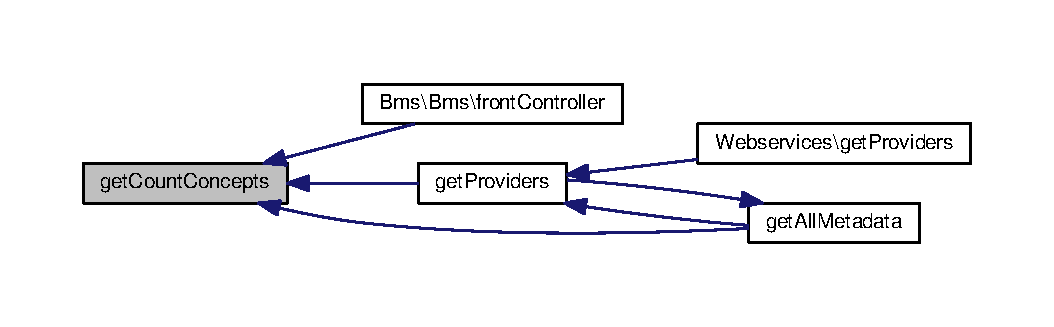
\includegraphics[width=350pt]{backend_8js_a46a518d9683fe224cd47219f3da32d07_icgraph}
\end{center}
\end{figure}


\index{backend.\+js@{backend.\+js}!get\+Data\+Set\+Titles@{get\+Data\+Set\+Titles}}
\index{get\+Data\+Set\+Titles@{get\+Data\+Set\+Titles}!backend.\+js@{backend.\+js}}
\subsubsection[{\texorpdfstring{get\+Data\+Set\+Titles(id\+D\+S\+A, url, dataset)}{getDataSetTitles(idDSA, url, dataset)}}]{\setlength{\rightskip}{0pt plus 5cm}function get\+Data\+Set\+Titles (
\begin{DoxyParamCaption}
\item[{}]{id\+D\+SA, }
\item[{}]{url, }
\item[{}]{dataset}
\end{DoxyParamCaption}
)}\hypertarget{backend_8js_a82c76ce90ab8a91de559f9b35d0088d7}{}\label{backend_8js_a82c76ce90ab8a91de559f9b35d0088d7}
get Dataset titles


\begin{DoxyParams}[1]{Parameters}
int & {\em \$id\+D\+SA} & \\
\hline
string & {\em \$url} & complete Query U\+RL incl. ?dsa=xxx \\
\hline
int & {\em \$id\+D\+SA} & \\
\hline
string & {\em \$data\+Set} & \\
\hline
\end{DoxyParams}
\begin{DoxyReturn}{Returns}
void 
\end{DoxyReturn}


Definition at line 235 of file backend.\+js.



Here is the caller graph for this function\+:\nopagebreak
\begin{figure}[H]
\begin{center}
\leavevmode
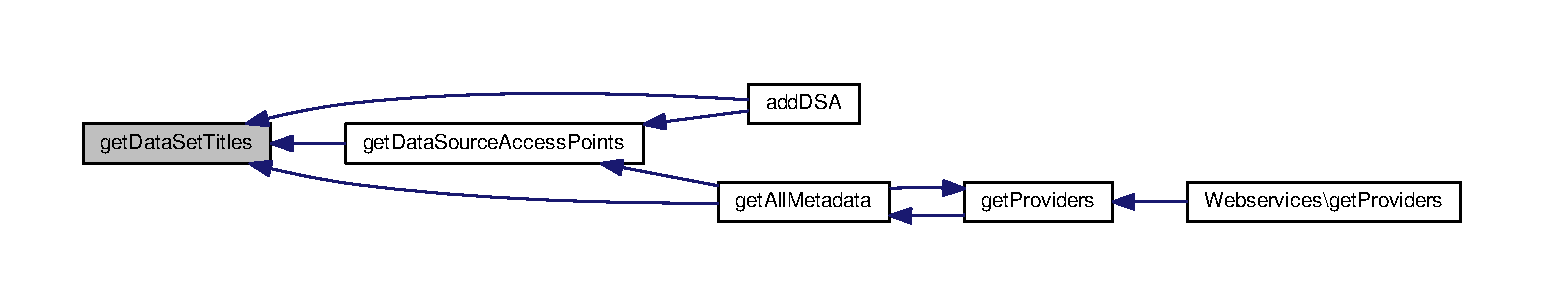
\includegraphics[width=350pt]{backend_8js_a82c76ce90ab8a91de559f9b35d0088d7_icgraph}
\end{center}
\end{figure}


\index{backend.\+js@{backend.\+js}!get\+Data\+Source\+Access\+Points@{get\+Data\+Source\+Access\+Points}}
\index{get\+Data\+Source\+Access\+Points@{get\+Data\+Source\+Access\+Points}!backend.\+js@{backend.\+js}}
\subsubsection[{\texorpdfstring{get\+Data\+Source\+Access\+Points(id\+Provider, url, id\+D\+S\+A, selected\+Value, data\+Set)}{getDataSourceAccessPoints(idProvider, url, idDSA, selectedValue, dataSet)}}]{\setlength{\rightskip}{0pt plus 5cm}function get\+Data\+Source\+Access\+Points (
\begin{DoxyParamCaption}
\item[{}]{id\+Provider, }
\item[{}]{url, }
\item[{}]{id\+D\+SA, }
\item[{}]{selected\+Value, }
\item[{}]{data\+Set}
\end{DoxyParamCaption}
)}\hypertarget{backend_8js_a06ed191b32ca45ffc8c3ad30bf6f6cf4}{}\label{backend_8js_a06ed191b32ca45ffc8c3ad30bf6f6cf4}
get Data Source Access (D\+SA) Points and Data\+Set Titles


\begin{DoxyParams}[1]{Parameters}
int & {\em \$id\+Provider} & \\
\hline
string & {\em \$url} & complete Query U\+RL incl. ?dsa=xxx \\
\hline
int & {\em \$id\+D\+SA} & \\
\hline
string & {\em \$selected\+Value} & previously selected Data\+Set \\
\hline
string & {\em \$data\+Set} & \\
\hline
\end{DoxyParams}
\begin{DoxyReturn}{Returns}
void 
\end{DoxyReturn}


Definition at line 180 of file backend.\+js.



Here is the call graph for this function\+:\nopagebreak
\begin{figure}[H]
\begin{center}
\leavevmode
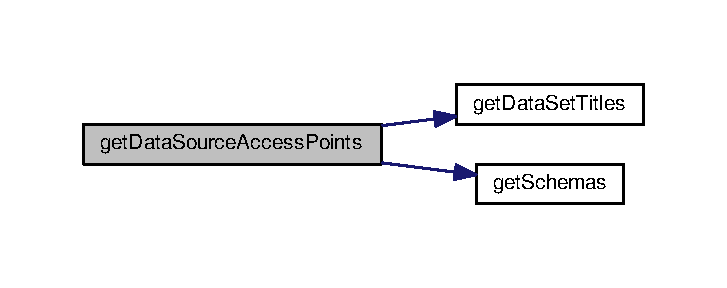
\includegraphics[width=349pt]{backend_8js_a06ed191b32ca45ffc8c3ad30bf6f6cf4_cgraph}
\end{center}
\end{figure}




Here is the caller graph for this function\+:\nopagebreak
\begin{figure}[H]
\begin{center}
\leavevmode
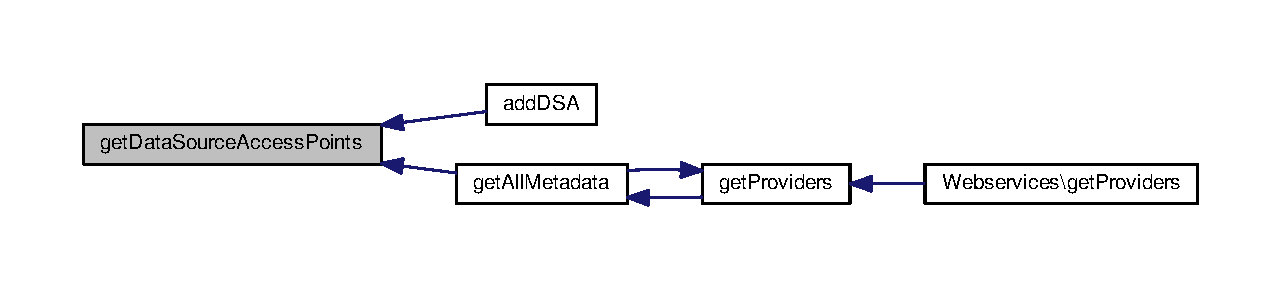
\includegraphics[width=350pt]{backend_8js_a06ed191b32ca45ffc8c3ad30bf6f6cf4_icgraph}
\end{center}
\end{figure}


\index{backend.\+js@{backend.\+js}!get\+Link\+Categories@{get\+Link\+Categories}}
\index{get\+Link\+Categories@{get\+Link\+Categories}!backend.\+js@{backend.\+js}}
\subsubsection[{\texorpdfstring{get\+Link\+Categories()}{getLinkCategories()}}]{\setlength{\rightskip}{0pt plus 5cm}function get\+Link\+Categories (
\begin{DoxyParamCaption}
{}
\end{DoxyParamCaption}
)}\hypertarget{backend_8js_af5cbf7c37f28fddd8b8a5149a7ed5900}{}\label{backend_8js_af5cbf7c37f28fddd8b8a5149a7ed5900}
get all link categories

\begin{DoxyReturn}{Returns}
\{void\} 
\end{DoxyReturn}


Definition at line 1102 of file backend.\+js.



Here is the caller graph for this function\+:\nopagebreak
\begin{figure}[H]
\begin{center}
\leavevmode
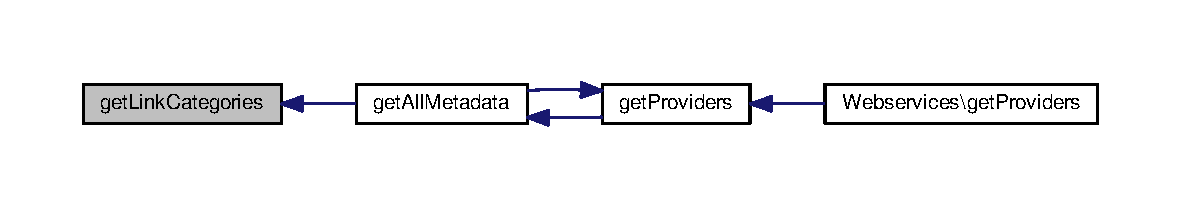
\includegraphics[width=350pt]{backend_8js_af5cbf7c37f28fddd8b8a5149a7ed5900_icgraph}
\end{center}
\end{figure}


\index{backend.\+js@{backend.\+js}!get\+Providers@{get\+Providers}}
\index{get\+Providers@{get\+Providers}!backend.\+js@{backend.\+js}}
\subsubsection[{\texorpdfstring{get\+Providers()}{getProviders()}}]{\setlength{\rightskip}{0pt plus 5cm}function get\+Providers (
\begin{DoxyParamCaption}
{}
\end{DoxyParamCaption}
)}\hypertarget{backend_8js_a6879c4dc7db6793991cd72ab19ca85ea}{}\label{backend_8js_a6879c4dc7db6793991cd72ab19ca85ea}
get list of providers

\begin{DoxyReturn}{Returns}
boolean false 
\end{DoxyReturn}


Definition at line 35 of file backend.\+js.



Here is the call graph for this function\+:\nopagebreak
\begin{figure}[H]
\begin{center}
\leavevmode
\includegraphics[width=350pt]{backend_8js_a6879c4dc7db6793991cd72ab19ca85ea_cgraph}
\end{center}
\end{figure}




Here is the caller graph for this function\+:\nopagebreak
\begin{figure}[H]
\begin{center}
\leavevmode
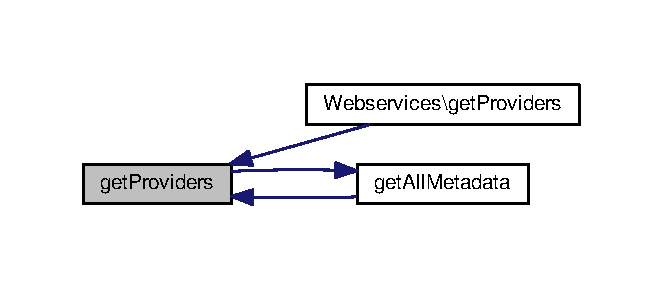
\includegraphics[width=318pt]{backend_8js_a6879c4dc7db6793991cd72ab19ca85ea_icgraph}
\end{center}
\end{figure}


\index{backend.\+js@{backend.\+js}!get\+Schemas@{get\+Schemas}}
\index{get\+Schemas@{get\+Schemas}!backend.\+js@{backend.\+js}}
\subsubsection[{\texorpdfstring{get\+Schemas(id\+Provider, id\+D\+S\+A, dsa, selected\+Value)}{getSchemas(idProvider, idDSA, dsa, selectedValue)}}]{\setlength{\rightskip}{0pt plus 5cm}function get\+Schemas (
\begin{DoxyParamCaption}
\item[{}]{id\+Provider, }
\item[{}]{id\+D\+SA, }
\item[{}]{dsa, }
\item[{}]{selected\+Value}
\end{DoxyParamCaption}
)}\hypertarget{backend_8js_a51fe50f57ea6df6fb0bcbd22099962ab}{}\label{backend_8js_a51fe50f57ea6df6fb0bcbd22099962ab}
get schemas via capabilities request


\begin{DoxyParams}[1]{Parameters}
int & {\em \$id\+Provider} & \\
\hline
int & {\em \$id\+D\+SA} & \\
\hline
 & {\em string} & \$\$dsa \\
\hline
 & {\em string} & \$\$selected\+Value \\
\hline
\end{DoxyParams}
\begin{DoxyReturn}{Returns}
void 
\end{DoxyReturn}


Definition at line 110 of file backend.\+js.



Here is the caller graph for this function\+:\nopagebreak
\begin{figure}[H]
\begin{center}
\leavevmode
\includegraphics[width=350pt]{backend_8js_a51fe50f57ea6df6fb0bcbd22099962ab_icgraph}
\end{center}
\end{figure}


\index{backend.\+js@{backend.\+js}!get\+Useful\+Links@{get\+Useful\+Links}}
\index{get\+Useful\+Links@{get\+Useful\+Links}!backend.\+js@{backend.\+js}}
\subsubsection[{\texorpdfstring{get\+Useful\+Links(id\+Provider, id\+D\+S\+A)}{getUsefulLinks(idProvider, idDSA)}}]{\setlength{\rightskip}{0pt plus 5cm}function get\+Useful\+Links (
\begin{DoxyParamCaption}
\item[{}]{id\+Provider, }
\item[{}]{id\+D\+SA}
\end{DoxyParamCaption}
)}\hypertarget{backend_8js_add7d88a4ad05a1fb2478eff9a1857824}{}\label{backend_8js_add7d88a4ad05a1fb2478eff9a1857824}
gets the useful Links of a given D\+SA


\begin{DoxyParams}[1]{Parameters}
int & {\em \$id\+Provider} & \\
\hline
int & {\em \$id\+D\+SA} & \\
\hline
\end{DoxyParams}
\begin{DoxyReturn}{Returns}
boolean false 
\end{DoxyReturn}


Definition at line 1416 of file backend.\+js.



Here is the caller graph for this function\+:\nopagebreak
\begin{figure}[H]
\begin{center}
\leavevmode
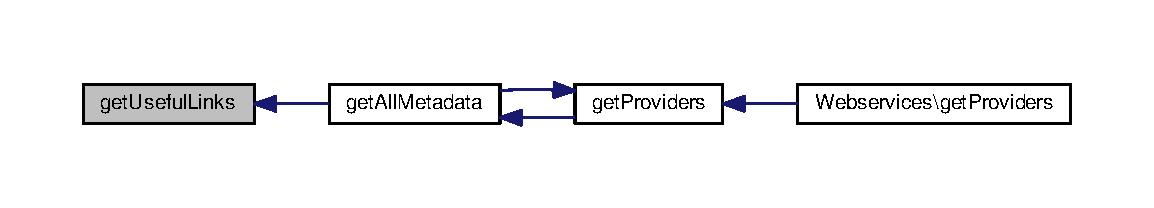
\includegraphics[width=350pt]{backend_8js_add7d88a4ad05a1fb2478eff9a1857824_icgraph}
\end{center}
\end{figure}


\index{backend.\+js@{backend.\+js}!hide\+Archive@{hide\+Archive}}
\index{hide\+Archive@{hide\+Archive}!backend.\+js@{backend.\+js}}
\subsubsection[{\texorpdfstring{hide\+Archive(id\+D\+S\+A, id, counter)}{hideArchive(idDSA, id, counter)}}]{\setlength{\rightskip}{0pt plus 5cm}function hide\+Archive (
\begin{DoxyParamCaption}
\item[{}]{id\+D\+SA, }
\item[{}]{id, }
\item[{}]{counter}
\end{DoxyParamCaption}
)}\hypertarget{backend_8js_a15d235044db55b8761af5c59ac1673a1}{}\label{backend_8js_a15d235044db55b8761af5c59ac1673a1}
hides an Archive


\begin{DoxyParams}[1]{Parameters}
int & {\em \$id\+D\+SA} & ID of Data Source Access Point \\
\hline
int & {\em \$id} & ID of Archive \\
\hline
int & {\em \$counter} & list item counter \\
\hline
\end{DoxyParams}
\begin{DoxyReturn}{Returns}
void 
\end{DoxyReturn}


Definition at line 903 of file backend.\+js.

\index{backend.\+js@{backend.\+js}!hide\+Useful\+Link@{hide\+Useful\+Link}}
\index{hide\+Useful\+Link@{hide\+Useful\+Link}!backend.\+js@{backend.\+js}}
\subsubsection[{\texorpdfstring{hide\+Useful\+Link(id\+D\+S\+A, id)}{hideUsefulLink(idDSA, id)}}]{\setlength{\rightskip}{0pt plus 5cm}function hide\+Useful\+Link (
\begin{DoxyParamCaption}
\item[{}]{id\+D\+SA, }
\item[{}]{id}
\end{DoxyParamCaption}
)}\hypertarget{backend_8js_a6f43dd08d697f48f45ed08af494d9367}{}\label{backend_8js_a6f43dd08d697f48f45ed08af494d9367}
hides a Useful Link


\begin{DoxyParams}[1]{Parameters}
int & {\em \$id\+D\+SA} & ID of Data Source Access Point \\
\hline
int & {\em \$id} & ID of Useful Link \\
\hline
\end{DoxyParams}
\begin{DoxyReturn}{Returns}
void 
\end{DoxyReturn}


Definition at line 1018 of file backend.\+js.

\index{backend.\+js@{backend.\+js}!remove\+Archive@{remove\+Archive}}
\index{remove\+Archive@{remove\+Archive}!backend.\+js@{backend.\+js}}
\subsubsection[{\texorpdfstring{remove\+Archive(id\+D\+S\+A, id)}{removeArchive(idDSA, id)}}]{\setlength{\rightskip}{0pt plus 5cm}function remove\+Archive (
\begin{DoxyParamCaption}
\item[{}]{id\+D\+SA, }
\item[{}]{id}
\end{DoxyParamCaption}
)}\hypertarget{backend_8js_a67ccb2b34eb0513b50335e24a6b20d40}{}\label{backend_8js_a67ccb2b34eb0513b50335e24a6b20d40}
removes an Archive


\begin{DoxyParams}[1]{Parameters}
int & {\em \$id\+D\+SA} & ID of Data Source Access Point \\
\hline
int & {\em \$id} & ID of Archive \\
\hline
\end{DoxyParams}
\begin{DoxyReturn}{Returns}
void 
\end{DoxyReturn}


Definition at line 929 of file backend.\+js.



Here is the call graph for this function\+:\nopagebreak
\begin{figure}[H]
\begin{center}
\leavevmode
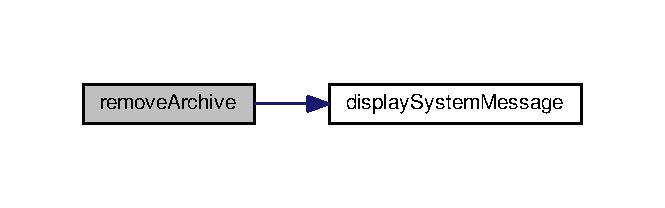
\includegraphics[width=319pt]{backend_8js_a67ccb2b34eb0513b50335e24a6b20d40_cgraph}
\end{center}
\end{figure}


\index{backend.\+js@{backend.\+js}!remove\+Count@{remove\+Count}}
\index{remove\+Count@{remove\+Count}!backend.\+js@{backend.\+js}}
\subsubsection[{\texorpdfstring{remove\+Count(id)}{removeCount(id)}}]{\setlength{\rightskip}{0pt plus 5cm}function remove\+Count (
\begin{DoxyParamCaption}
\item[{}]{id}
\end{DoxyParamCaption}
)}\hypertarget{backend_8js_aa19813ae51cc1b506e8543a7cd6a0e42}{}\label{backend_8js_aa19813ae51cc1b506e8543a7cd6a0e42}
removes a Count Concept


\begin{DoxyParams}[1]{Parameters}
int & {\em \$id} & a Count Concept \\
\hline
\end{DoxyParams}
\begin{DoxyReturn}{Returns}
void 
\end{DoxyReturn}


Definition at line 746 of file backend.\+js.



Here is the call graph for this function\+:\nopagebreak
\begin{figure}[H]
\begin{center}
\leavevmode
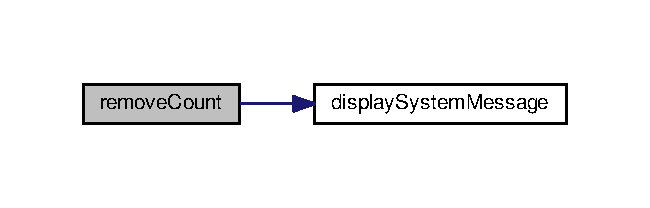
\includegraphics[width=312pt]{backend_8js_aa19813ae51cc1b506e8543a7cd6a0e42_cgraph}
\end{center}
\end{figure}


\index{backend.\+js@{backend.\+js}!remove\+D\+SA@{remove\+D\+SA}}
\index{remove\+D\+SA@{remove\+D\+SA}!backend.\+js@{backend.\+js}}
\subsubsection[{\texorpdfstring{remove\+D\+S\+A(id)}{removeDSA(id)}}]{\setlength{\rightskip}{0pt plus 5cm}function remove\+D\+SA (
\begin{DoxyParamCaption}
\item[{}]{id}
\end{DoxyParamCaption}
)}\hypertarget{backend_8js_a36b49b10ca5bff2748b29988f1582f34}{}\label{backend_8js_a36b49b10ca5bff2748b29988f1582f34}
removes a given D\+SA


\begin{DoxyParams}[1]{Parameters}
int & {\em \$id} & id\+D\+SA \\
\hline
\end{DoxyParams}
\begin{DoxyReturn}{Returns}
void 
\end{DoxyReturn}


Definition at line 660 of file backend.\+js.



Here is the call graph for this function\+:\nopagebreak
\begin{figure}[H]
\begin{center}
\leavevmode
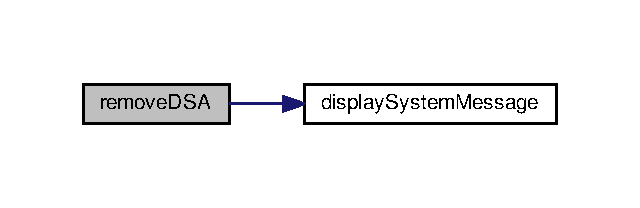
\includegraphics[width=307pt]{backend_8js_a36b49b10ca5bff2748b29988f1582f34_cgraph}
\end{center}
\end{figure}


\index{backend.\+js@{backend.\+js}!remove\+Useful\+Link@{remove\+Useful\+Link}}
\index{remove\+Useful\+Link@{remove\+Useful\+Link}!backend.\+js@{backend.\+js}}
\subsubsection[{\texorpdfstring{remove\+Useful\+Link(id\+D\+S\+A, id)}{removeUsefulLink(idDSA, id)}}]{\setlength{\rightskip}{0pt plus 5cm}function remove\+Useful\+Link (
\begin{DoxyParamCaption}
\item[{}]{id\+D\+SA, }
\item[{}]{id}
\end{DoxyParamCaption}
)}\hypertarget{backend_8js_a2b6e8bcc79cbc217976969a2c3830205}{}\label{backend_8js_a2b6e8bcc79cbc217976969a2c3830205}
removes a Useful Link


\begin{DoxyParams}[1]{Parameters}
int & {\em \$id\+D\+SA} & ID of Data Source Access Point \\
\hline
int & {\em \$id} & ID of Useful Link \\
\hline
\end{DoxyParams}
\begin{DoxyReturn}{Returns}
void 
\end{DoxyReturn}


Definition at line 1032 of file backend.\+js.



Here is the call graph for this function\+:\nopagebreak
\begin{figure}[H]
\begin{center}
\leavevmode
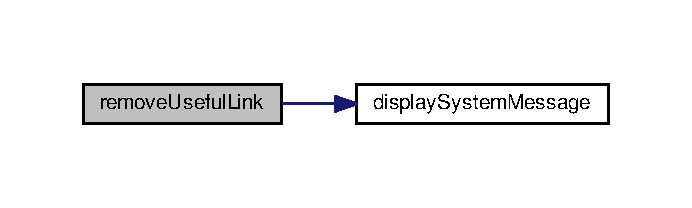
\includegraphics[width=332pt]{backend_8js_a2b6e8bcc79cbc217976969a2c3830205_cgraph}
\end{center}
\end{figure}


\index{backend.\+js@{backend.\+js}!save\+Archive@{save\+Archive}}
\index{save\+Archive@{save\+Archive}!backend.\+js@{backend.\+js}}
\subsubsection[{\texorpdfstring{save\+Archive(id\+Provider, id\+D\+S\+A, id)}{saveArchive(idProvider, idDSA, id)}}]{\setlength{\rightskip}{0pt plus 5cm}function save\+Archive (
\begin{DoxyParamCaption}
\item[{}]{id\+Provider, }
\item[{}]{id\+D\+SA, }
\item[{}]{id}
\end{DoxyParamCaption}
)}\hypertarget{backend_8js_a855d7bfb70d494b3a5937f118e0b4e60}{}\label{backend_8js_a855d7bfb70d494b3a5937f118e0b4e60}
saves an Archive


\begin{DoxyParams}[1]{Parameters}
int & {\em \$id\+Provider} & ID of Provider \\
\hline
int & {\em \$id\+D\+SA} & ID of Data Source Access Point \\
\hline
int & {\em \$id} & ID of Archive \\
\hline
\end{DoxyParams}
\begin{DoxyReturn}{Returns}
void 
\end{DoxyReturn}


Definition at line 858 of file backend.\+js.



Here is the call graph for this function\+:\nopagebreak
\begin{figure}[H]
\begin{center}
\leavevmode
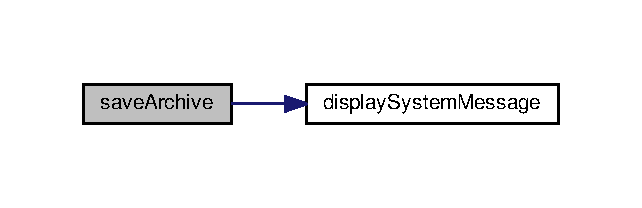
\includegraphics[width=308pt]{backend_8js_a855d7bfb70d494b3a5937f118e0b4e60_cgraph}
\end{center}
\end{figure}


\index{backend.\+js@{backend.\+js}!save\+Count@{save\+Count}}
\index{save\+Count@{save\+Count}!backend.\+js@{backend.\+js}}
\subsubsection[{\texorpdfstring{save\+Count(id)}{saveCount(id)}}]{\setlength{\rightskip}{0pt plus 5cm}function save\+Count (
\begin{DoxyParamCaption}
\item[{}]{id}
\end{DoxyParamCaption}
)}\hypertarget{backend_8js_af64a4f08a169e74e835e8779804d2982}{}\label{backend_8js_af64a4f08a169e74e835e8779804d2982}
saves a Count Concept


\begin{DoxyParams}[1]{Parameters}
int & {\em \$id} & a Count Concept \\
\hline
\end{DoxyParams}
\begin{DoxyReturn}{Returns}
void 
\end{DoxyReturn}


Definition at line 773 of file backend.\+js.



Here is the call graph for this function\+:\nopagebreak
\begin{figure}[H]
\begin{center}
\leavevmode
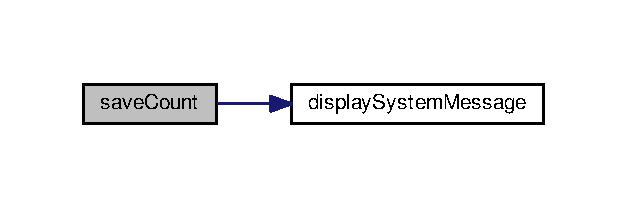
\includegraphics[width=301pt]{backend_8js_af64a4f08a169e74e835e8779804d2982_cgraph}
\end{center}
\end{figure}


\index{backend.\+js@{backend.\+js}!save\+D\+S\+A\+Point@{save\+D\+S\+A\+Point}}
\index{save\+D\+S\+A\+Point@{save\+D\+S\+A\+Point}!backend.\+js@{backend.\+js}}
\subsubsection[{\texorpdfstring{save\+D\+S\+A\+Point(dsa, reload)}{saveDSAPoint(dsa, reload)}}]{\setlength{\rightskip}{0pt plus 5cm}function save\+D\+S\+A\+Point (
\begin{DoxyParamCaption}
\item[{}]{dsa, }
\item[{}]{reload}
\end{DoxyParamCaption}
)}\hypertarget{backend_8js_ab8857c782e0fd01946658e1a47bd295c}{}\label{backend_8js_ab8857c782e0fd01946658e1a47bd295c}
stores a given D\+SA in the database


\begin{DoxyParams}{Parameters}
{\em \{object\}} & dsa object holding all fields \\
\hline
{\em \{boolean\}} & reload page? \\
\hline
\end{DoxyParams}
\begin{DoxyReturn}{Returns}
void 
\end{DoxyReturn}


Definition at line 578 of file backend.\+js.



Here is the call graph for this function\+:\nopagebreak
\begin{figure}[H]
\begin{center}
\leavevmode
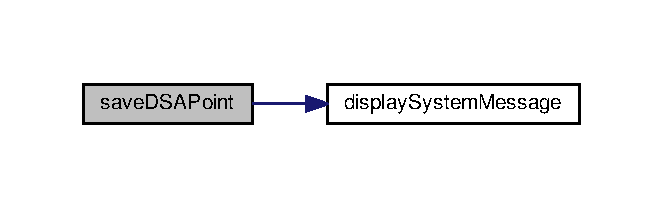
\includegraphics[width=318pt]{backend_8js_ab8857c782e0fd01946658e1a47bd295c_cgraph}
\end{center}
\end{figure}




Here is the caller graph for this function\+:\nopagebreak
\begin{figure}[H]
\begin{center}
\leavevmode
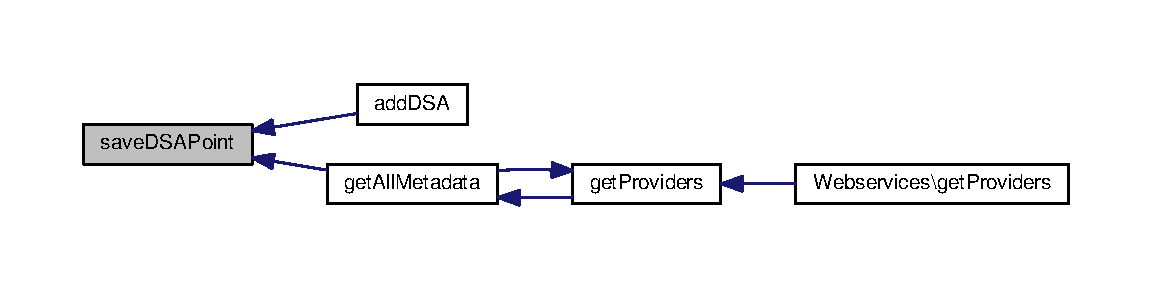
\includegraphics[width=350pt]{backend_8js_ab8857c782e0fd01946658e1a47bd295c_icgraph}
\end{center}
\end{figure}


\index{backend.\+js@{backend.\+js}!save\+Main\+Metadata@{save\+Main\+Metadata}}
\index{save\+Main\+Metadata@{save\+Main\+Metadata}!backend.\+js@{backend.\+js}}
\subsubsection[{\texorpdfstring{save\+Main\+Metadata()}{saveMainMetadata()}}]{\setlength{\rightskip}{0pt plus 5cm}function save\+Main\+Metadata (
\begin{DoxyParamCaption}
{}
\end{DoxyParamCaption}
)}\hypertarget{backend_8js_ad8bb15255910bba8451a623c74323537}{}\label{backend_8js_ad8bb15255910bba8451a623c74323537}
save Main Data of Provider

\begin{DoxyReturn}{Returns}
void 
\end{DoxyReturn}


Definition at line 81 of file backend.\+js.



Here is the call graph for this function\+:\nopagebreak
\begin{figure}[H]
\begin{center}
\leavevmode
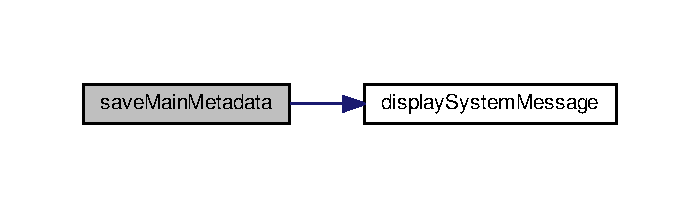
\includegraphics[width=336pt]{backend_8js_ad8bb15255910bba8451a623c74323537_cgraph}
\end{center}
\end{figure}


\index{backend.\+js@{backend.\+js}!save\+Useful\+Link@{save\+Useful\+Link}}
\index{save\+Useful\+Link@{save\+Useful\+Link}!backend.\+js@{backend.\+js}}
\subsubsection[{\texorpdfstring{save\+Useful\+Link(id\+Provider, id\+D\+S\+A, id)}{saveUsefulLink(idProvider, idDSA, id)}}]{\setlength{\rightskip}{0pt plus 5cm}function save\+Useful\+Link (
\begin{DoxyParamCaption}
\item[{}]{id\+Provider, }
\item[{}]{id\+D\+SA, }
\item[{}]{id}
\end{DoxyParamCaption}
)}\hypertarget{backend_8js_a9980fb97f36014ac0cf30b90df12498b}{}\label{backend_8js_a9980fb97f36014ac0cf30b90df12498b}
saves a Useful Link


\begin{DoxyParams}[1]{Parameters}
int & {\em \$id\+Provider} & ID of Provider \\
\hline
int & {\em \$id\+D\+SA} & ID of Data Source Access Point \\
\hline
int & {\em \$id} & ID of Useful Link \\
\hline
\end{DoxyParams}
\begin{DoxyReturn}{Returns}
void 
\end{DoxyReturn}


Definition at line 1061 of file backend.\+js.



Here is the call graph for this function\+:\nopagebreak
\begin{figure}[H]
\begin{center}
\leavevmode
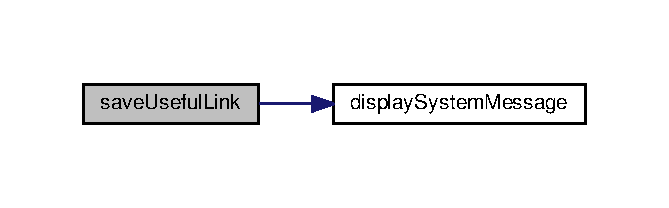
\includegraphics[width=321pt]{backend_8js_a9980fb97f36014ac0cf30b90df12498b_cgraph}
\end{center}
\end{figure}


\index{backend.\+js@{backend.\+js}!show\+Archive@{show\+Archive}}
\index{show\+Archive@{show\+Archive}!backend.\+js@{backend.\+js}}
\subsubsection[{\texorpdfstring{show\+Archive(id\+D\+S\+A, id)}{showArchive(idDSA, id)}}]{\setlength{\rightskip}{0pt plus 5cm}function show\+Archive (
\begin{DoxyParamCaption}
\item[{}]{id\+D\+SA, }
\item[{}]{id}
\end{DoxyParamCaption}
)}\hypertarget{backend_8js_afb708a6ab2f049a160aa9c65fb61bd75}{}\label{backend_8js_afb708a6ab2f049a160aa9c65fb61bd75}
shows an Archive


\begin{DoxyParams}[1]{Parameters}
int & {\em \$id\+D\+SA} & ID of Data Source Access Point \\
\hline
int & {\em \$id} & ID of Archive \\
\hline
\end{DoxyParams}
\begin{DoxyReturn}{Returns}
void 
\end{DoxyReturn}


Definition at line 917 of file backend.\+js.

\index{backend.\+js@{backend.\+js}!show\+Useful\+Link@{show\+Useful\+Link}}
\index{show\+Useful\+Link@{show\+Useful\+Link}!backend.\+js@{backend.\+js}}
\subsubsection[{\texorpdfstring{show\+Useful\+Link(id\+D\+S\+A, id)}{showUsefulLink(idDSA, id)}}]{\setlength{\rightskip}{0pt plus 5cm}function show\+Useful\+Link (
\begin{DoxyParamCaption}
\item[{}]{id\+D\+SA, }
\item[{}]{id}
\end{DoxyParamCaption}
)}\hypertarget{backend_8js_af3f3dcdc9df4e4491e80cbd1107f6d2d}{}\label{backend_8js_af3f3dcdc9df4e4491e80cbd1107f6d2d}
shows a Useful Link


\begin{DoxyParams}[1]{Parameters}
int & {\em \$id\+D\+SA} & ID of Data Source Access Point \\
\hline
int & {\em \$id} & ID of Useful Link \\
\hline
\end{DoxyParams}
\begin{DoxyReturn}{Returns}
void 
\end{DoxyReturn}


Definition at line 1006 of file backend.\+js.


\hypertarget{consistency_8js}{}\section{js/consistency.js File Reference}
\label{consistency_8js}\index{js/consistency.\+js@{js/consistency.\+js}}


javascript functions used in the consistency checker.  


\subsection*{Namespaces}
\begin{DoxyCompactItemize}
\item 
 \hyperlink{namespace_consistency}{Consistency}
\end{DoxyCompactItemize}
\subsection*{Functions}
\begin{DoxyCompactItemize}
\item 
function \hyperlink{consistency_8js_ae9dd19ed0c7bfeca794906a98cf25658}{get\+Unique} (input\+Array)
\item 
function \hyperlink{consistency_8js_afe73f65f5154e4738551f8fe2172e4e1}{match\+Rule} (function\+Name, url)
\item 
function \hyperlink{consistency_8js_a0cd14e63b9113fcee3fa0e999aa1ada9}{is\+Valid\+Citation} (str)
\item 
function \hyperlink{consistency_8js_a813c8c7bf883cb5ff071d2c59436ce1a}{check\+Rules} (id\+Provider, dsa, filter, mapping)
\item 
function \hyperlink{consistency_8js_abfdeb6a1262a6647fa8d1add87d4acff}{cardinal\+Concept} (id\+Provider, schema, filter, concept, j)
\item 
function \hyperlink{consistency_8js_a52ab9a53e64b869e116476df0f75c72c}{check\+For\+Errors} (id\+Provider, filter, concept, schema, mapping, j, total)
\item 
function \hyperlink{consistency_8js_ab9d69a98be46ebaa9c992bb5bea19199}{get\+Example\+Values} (provider, schema, url, filter, concept, j)
\item 
function \hyperlink{consistency_8js_ac57f515c2a7b72cd20b9a9a6526352c1}{extract\+Example\+Values} (event)
\item 
function \hyperlink{consistency_8js_a0e434d0abe4686a98fa7119ad3b98a23}{fire} (id\+Provider, dsa, filter)
\end{DoxyCompactItemize}


\subsection{Detailed Description}
This program is free software\+: you can redistribute it and/or modify it under the terms of the G\+NU General Public License as published by the Free Software Foundation, either version 3 of the License, or (at your option) any later version.

This program is distributed in the hope that it will be useful, but W\+I\+T\+H\+O\+UT A\+NY W\+A\+R\+R\+A\+N\+TY; without even the implied warranty of M\+E\+R\+C\+H\+A\+N\+T\+A\+B\+I\+L\+I\+TY or F\+I\+T\+N\+E\+SS F\+OR A P\+A\+R\+T\+I\+C\+U\+L\+AR P\+U\+R\+P\+O\+SE. See the G\+NU General Public License for more details.

You should have received a copy of the G\+NU General Public License along with this program. If not, see \href{http://www.gnu.org/licenses/}{\tt http\+://www.\+gnu.\+org/licenses/}.

The variables biocase\+Url and filter are defined in calling script \hyperlink{consistency_2index_8php}{biocasemonitor/consistency/index.\+php} 

\subsection{Function Documentation}
\index{consistency.\+js@{consistency.\+js}!cardinal\+Concept@{cardinal\+Concept}}
\index{cardinal\+Concept@{cardinal\+Concept}!consistency.\+js@{consistency.\+js}}
\subsubsection[{\texorpdfstring{cardinal\+Concept(id\+Provider, schema, filter, concept, j)}{cardinalConcept(idProvider, schema, filter, concept, j)}}]{\setlength{\rightskip}{0pt plus 5cm}function cardinal\+Concept (
\begin{DoxyParamCaption}
\item[{}]{id\+Provider, }
\item[{}]{schema, }
\item[{}]{filter, }
\item[{}]{concept, }
\item[{}]{j}
\end{DoxyParamCaption}
)}\hypertarget{consistency_8js_abfdeb6a1262a6647fa8d1add87d4acff}{}\label{consistency_8js_abfdeb6a1262a6647fa8d1add87d4acff}
counts the number of entries satisfying a given concept


\begin{DoxyParams}[1]{Parameters}
int & {\em \$id\+Provider} & \\
\hline
string & {\em \$schema} & \\
\hline
string & {\em \$filter} & a complex filter\+: $<$like$>$....$<$/like$>$ \\
\hline
string & {\em \$concept} & a capability. e.\+g.\+: /\+Data\+Sets/\+Data\+Set/\+Units/\+Unit/\+Unit\+ID \\
\hline
int & {\em \$j} & row number \\
\hline
\end{DoxyParams}
\begin{DoxyReturn}{Returns}
boolean false 
\end{DoxyReturn}


Definition at line 314 of file consistency.\+js.



Here is the caller graph for this function\+:\nopagebreak
\begin{figure}[H]
\begin{center}
\leavevmode
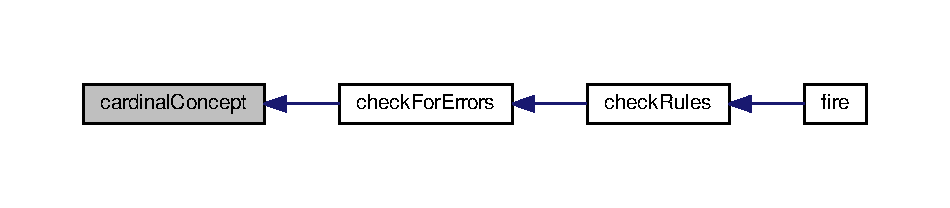
\includegraphics[width=350pt]{consistency_8js_abfdeb6a1262a6647fa8d1add87d4acff_icgraph}
\end{center}
\end{figure}


\index{consistency.\+js@{consistency.\+js}!check\+For\+Errors@{check\+For\+Errors}}
\index{check\+For\+Errors@{check\+For\+Errors}!consistency.\+js@{consistency.\+js}}
\subsubsection[{\texorpdfstring{check\+For\+Errors(id\+Provider, filter, concept, schema, mapping, j, total)}{checkForErrors(idProvider, filter, concept, schema, mapping, j, total)}}]{\setlength{\rightskip}{0pt plus 5cm}function check\+For\+Errors (
\begin{DoxyParamCaption}
\item[{}]{id\+Provider, }
\item[{}]{filter, }
\item[{}]{concept, }
\item[{}]{schema, }
\item[{}]{mapping, }
\item[{}]{j, }
\item[{}]{total}
\end{DoxyParamCaption}
)}\hypertarget{consistency_8js_a52ab9a53e64b869e116476df0f75c72c}{}\label{consistency_8js_a52ab9a53e64b869e116476df0f75c72c}
check concept entry for consistency


\begin{DoxyParams}[1]{Parameters}
int & {\em \$id\+Provider} & \\
\hline
string & {\em \$filter} & a complex filter\+: $<$like$>$....$<$/like$>$ \\
\hline
string & {\em \$concept} & a capability. e.\+g.\+: /\+Data\+Sets/\+Data\+Set/\+Units/\+Unit/\+Unit\+ID \\
\hline
string & {\em \$schema} & \\
\hline
string & {\em \$mapping} & \\
\hline
int & {\em \$j} & number of displayed row \\
\hline
int & {\em \$total} & total number \\
\hline
\end{DoxyParams}
\begin{DoxyReturn}{Returns}
boolean false 
\end{DoxyReturn}


Definition at line 368 of file consistency.\+js.



Here is the call graph for this function\+:\nopagebreak
\begin{figure}[H]
\begin{center}
\leavevmode
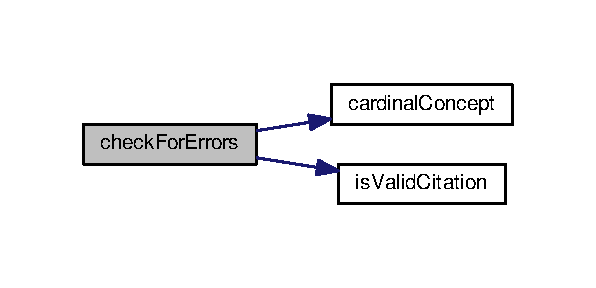
\includegraphics[width=286pt]{consistency_8js_a52ab9a53e64b869e116476df0f75c72c_cgraph}
\end{center}
\end{figure}




Here is the caller graph for this function\+:\nopagebreak
\begin{figure}[H]
\begin{center}
\leavevmode
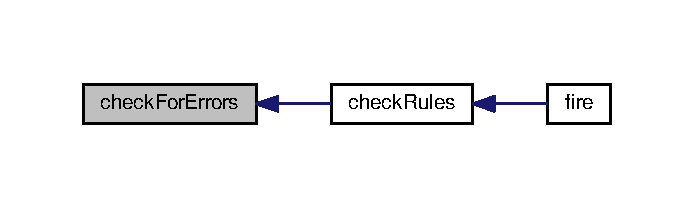
\includegraphics[width=333pt]{consistency_8js_a52ab9a53e64b869e116476df0f75c72c_icgraph}
\end{center}
\end{figure}


\index{consistency.\+js@{consistency.\+js}!check\+Rules@{check\+Rules}}
\index{check\+Rules@{check\+Rules}!consistency.\+js@{consistency.\+js}}
\subsubsection[{\texorpdfstring{check\+Rules(id\+Provider, dsa, filter, mapping)}{checkRules(idProvider, dsa, filter, mapping)}}]{\setlength{\rightskip}{0pt plus 5cm}function check\+Rules (
\begin{DoxyParamCaption}
\item[{}]{id\+Provider, }
\item[{}]{dsa, }
\item[{}]{filter, }
\item[{}]{mapping}
\end{DoxyParamCaption}
)}\hypertarget{consistency_8js_a813c8c7bf883cb5ff071d2c59436ce1a}{}\label{consistency_8js_a813c8c7bf883cb5ff071d2c59436ce1a}
check rules


\begin{DoxyParams}[1]{Parameters}
int & {\em \$id\+Provider} & \\
\hline
string & {\em \$dsa} & \\
\hline
string & {\em \$filter} & \\
\hline
string & {\em \$mapping} & \\
\hline
\end{DoxyParams}
\begin{DoxyReturn}{Returns}
object 
\end{DoxyReturn}


Definition at line 116 of file consistency.\+js.



Here is the call graph for this function\+:\nopagebreak
\begin{figure}[H]
\begin{center}
\leavevmode
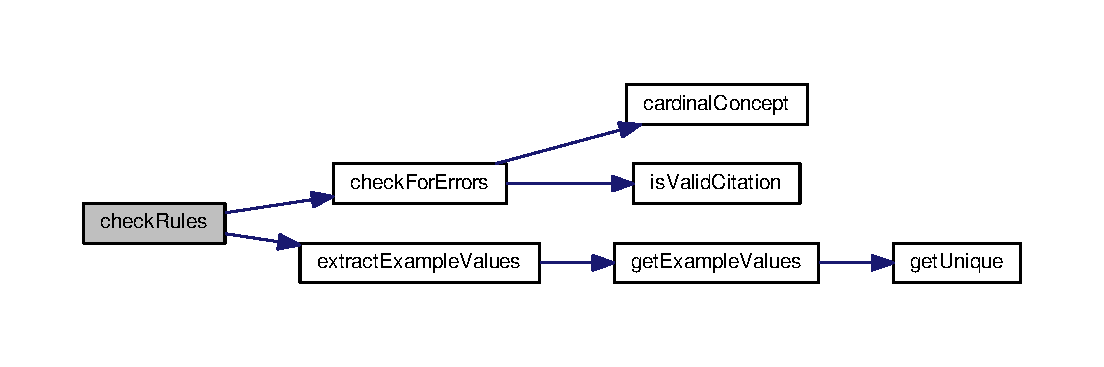
\includegraphics[width=350pt]{consistency_8js_a813c8c7bf883cb5ff071d2c59436ce1a_cgraph}
\end{center}
\end{figure}




Here is the caller graph for this function\+:\nopagebreak
\begin{figure}[H]
\begin{center}
\leavevmode
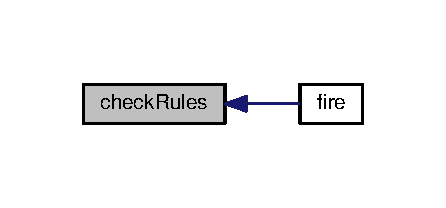
\includegraphics[width=214pt]{consistency_8js_a813c8c7bf883cb5ff071d2c59436ce1a_icgraph}
\end{center}
\end{figure}


\index{consistency.\+js@{consistency.\+js}!extract\+Example\+Values@{extract\+Example\+Values}}
\index{extract\+Example\+Values@{extract\+Example\+Values}!consistency.\+js@{consistency.\+js}}
\subsubsection[{\texorpdfstring{extract\+Example\+Values(event)}{extractExampleValues(event)}}]{\setlength{\rightskip}{0pt plus 5cm}function extract\+Example\+Values (
\begin{DoxyParamCaption}
\item[{}]{event}
\end{DoxyParamCaption}
)}\hypertarget{consistency_8js_ac57f515c2a7b72cd20b9a9a6526352c1}{}\label{consistency_8js_ac57f515c2a7b72cd20b9a9a6526352c1}
gets some example values of entries , called on\+Click.


\begin{DoxyParams}{Parameters}
{\em \{object\}} & event \\
\hline
\end{DoxyParams}
\begin{DoxyReturn}{Returns}
boolean false 
\end{DoxyReturn}


Definition at line 588 of file consistency.\+js.



Here is the call graph for this function\+:\nopagebreak
\begin{figure}[H]
\begin{center}
\leavevmode
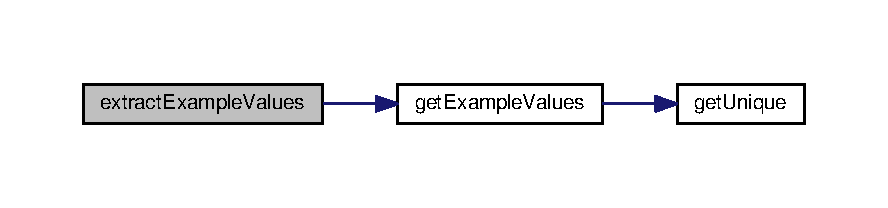
\includegraphics[width=350pt]{consistency_8js_ac57f515c2a7b72cd20b9a9a6526352c1_cgraph}
\end{center}
\end{figure}




Here is the caller graph for this function\+:\nopagebreak
\begin{figure}[H]
\begin{center}
\leavevmode
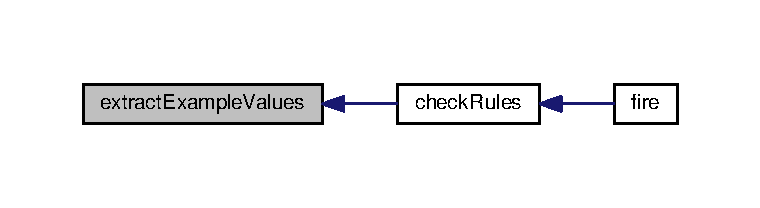
\includegraphics[width=350pt]{consistency_8js_ac57f515c2a7b72cd20b9a9a6526352c1_icgraph}
\end{center}
\end{figure}


\index{consistency.\+js@{consistency.\+js}!fire@{fire}}
\index{fire@{fire}!consistency.\+js@{consistency.\+js}}
\subsubsection[{\texorpdfstring{fire(id\+Provider, dsa, filter)}{fire(idProvider, dsa, filter)}}]{\setlength{\rightskip}{0pt plus 5cm}function fire (
\begin{DoxyParamCaption}
\item[{}]{id\+Provider, }
\item[{}]{dsa, }
\item[{}]{filter}
\end{DoxyParamCaption}
)}\hypertarget{consistency_8js_a0e434d0abe4686a98fa7119ad3b98a23}{}\label{consistency_8js_a0e434d0abe4686a98fa7119ad3b98a23}
gets all capabilities, checks against mandatory concepts, and populates the data table


\begin{DoxyEnumerate}
\item gets schema mapppings from DB
\item gets capabilities
\item extracts schemas from capabilities
\end{DoxyEnumerate}


\begin{DoxyParams}[1]{Parameters}
int & {\em \$id\+Provider} & \\
\hline
string & {\em \$dsa} & \\
\hline
string & {\em \$filter} & \\
\hline
\end{DoxyParams}
\begin{DoxyReturn}{Returns}
boolean false 
\end{DoxyReturn}


Definition at line 610 of file consistency.\+js.



Here is the call graph for this function\+:\nopagebreak
\begin{figure}[H]
\begin{center}
\leavevmode
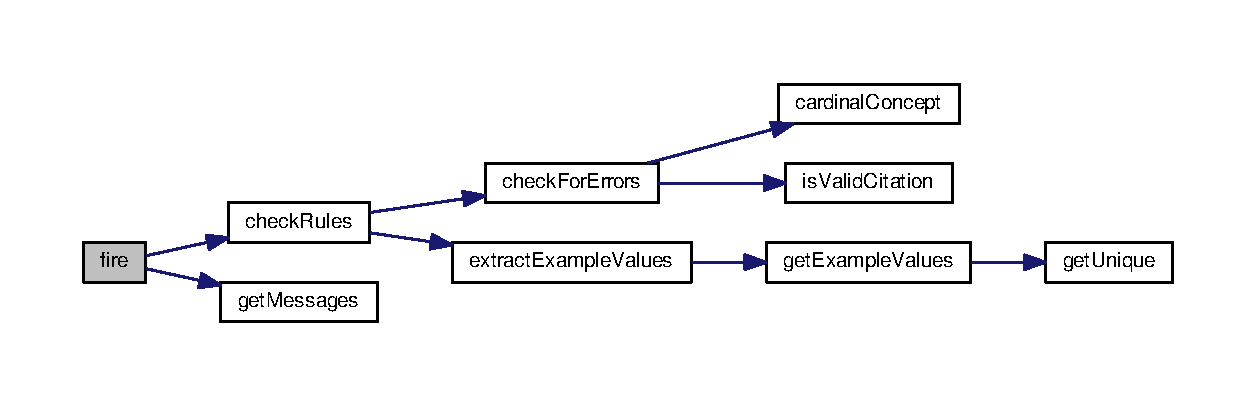
\includegraphics[width=350pt]{consistency_8js_a0e434d0abe4686a98fa7119ad3b98a23_cgraph}
\end{center}
\end{figure}


\index{consistency.\+js@{consistency.\+js}!get\+Example\+Values@{get\+Example\+Values}}
\index{get\+Example\+Values@{get\+Example\+Values}!consistency.\+js@{consistency.\+js}}
\subsubsection[{\texorpdfstring{get\+Example\+Values(provider, schema, url, filter, concept, j)}{getExampleValues(provider, schema, url, filter, concept, j)}}]{\setlength{\rightskip}{0pt plus 5cm}function get\+Example\+Values (
\begin{DoxyParamCaption}
\item[{}]{provider, }
\item[{}]{schema, }
\item[{}]{url, }
\item[{}]{filter, }
\item[{}]{concept, }
\item[{}]{j}
\end{DoxyParamCaption}
)}\hypertarget{consistency_8js_ab9d69a98be46ebaa9c992bb5bea19199}{}\label{consistency_8js_ab9d69a98be46ebaa9c992bb5bea19199}
gets example values of entries satisfying a given concept


\begin{DoxyParams}[1]{Parameters}
int & {\em \$provider} & id\+Provider \\
\hline
string & {\em \$schema} & data schema \\
\hline
string & {\em \$url} & query\+U\+RL \\
\hline
string & {\em \$filter} & a complex filter\+: $<$like$>$....$<$/like$>$ \\
\hline
string & {\em \$concept} & a capability. e.\+g.\+: /\+Data\+Sets/\+Data\+Set/\+Units/\+Unit/\+Unit\+ID \\
\hline
int & {\em \$j} & row number \\
\hline
\end{DoxyParams}
\begin{DoxyReturn}{Returns}
boolean false 
\end{DoxyReturn}


Definition at line 513 of file consistency.\+js.



Here is the call graph for this function\+:\nopagebreak
\begin{figure}[H]
\begin{center}
\leavevmode
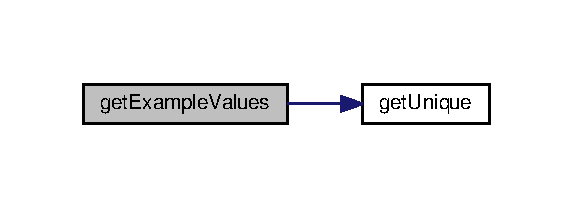
\includegraphics[width=275pt]{consistency_8js_ab9d69a98be46ebaa9c992bb5bea19199_cgraph}
\end{center}
\end{figure}




Here is the caller graph for this function\+:\nopagebreak
\begin{figure}[H]
\begin{center}
\leavevmode
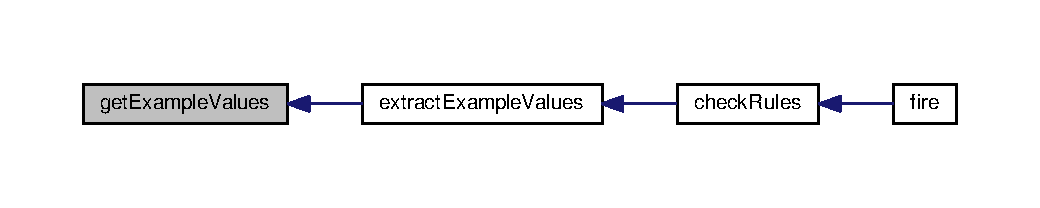
\includegraphics[width=350pt]{consistency_8js_ab9d69a98be46ebaa9c992bb5bea19199_icgraph}
\end{center}
\end{figure}


\index{consistency.\+js@{consistency.\+js}!get\+Unique@{get\+Unique}}
\index{get\+Unique@{get\+Unique}!consistency.\+js@{consistency.\+js}}
\subsubsection[{\texorpdfstring{get\+Unique(input\+Array)}{getUnique(inputArray)}}]{\setlength{\rightskip}{0pt plus 5cm}function get\+Unique (
\begin{DoxyParamCaption}
\item[{}]{input\+Array}
\end{DoxyParamCaption}
)}\hypertarget{consistency_8js_ae9dd19ed0c7bfeca794906a98cf25658}{}\label{consistency_8js_ae9dd19ed0c7bfeca794906a98cf25658}
removes redundant elements in an array


\begin{DoxyParams}[1]{Parameters}
array & {\em \$input\+Array} & \\
\hline
\end{DoxyParams}
\begin{DoxyReturn}{Returns}
Array 
\end{DoxyReturn}


Definition at line 36 of file consistency.\+js.



Here is the caller graph for this function\+:\nopagebreak
\begin{figure}[H]
\begin{center}
\leavevmode
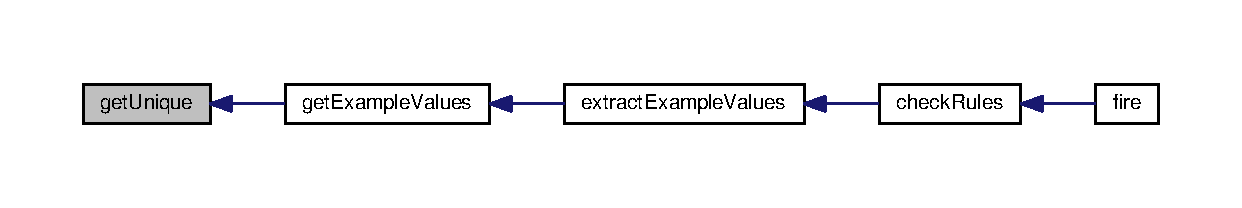
\includegraphics[width=350pt]{consistency_8js_ae9dd19ed0c7bfeca794906a98cf25658_icgraph}
\end{center}
\end{figure}


\index{consistency.\+js@{consistency.\+js}!is\+Valid\+Citation@{is\+Valid\+Citation}}
\index{is\+Valid\+Citation@{is\+Valid\+Citation}!consistency.\+js@{consistency.\+js}}
\subsubsection[{\texorpdfstring{is\+Valid\+Citation(str)}{isValidCitation(str)}}]{\setlength{\rightskip}{0pt plus 5cm}function is\+Valid\+Citation (
\begin{DoxyParamCaption}
\item[{}]{str}
\end{DoxyParamCaption}
)}\hypertarget{consistency_8js_a0cd14e63b9113fcee3fa0e999aa1ada9}{}\label{consistency_8js_a0cd14e63b9113fcee3fa0e999aa1ada9}
validates Citation $<$\+Authors$>$. ($<$\+Publication\+\_\+year$>$). $<$\+Title$>$. \mbox{[}Dataset\mbox{]}. $<$\+Version\+Nr$>$. Data Publisher\+: $<$\+Data\+\_\+center\+\_\+name$>$. $<$\+U\+R\+I$>$. \begin{DoxyRefDesc}{Todo}
\item[\hyperlink{todo__todo000010}{Todo}]adapt to consensus document\end{DoxyRefDesc}



\begin{DoxyParams}[1]{Parameters}
string & {\em \$str} & \\
\hline
\end{DoxyParams}
\begin{DoxyReturn}{Returns}
boolean 
\end{DoxyReturn}


Definition at line 72 of file consistency.\+js.



Here is the caller graph for this function\+:\nopagebreak
\begin{figure}[H]
\begin{center}
\leavevmode
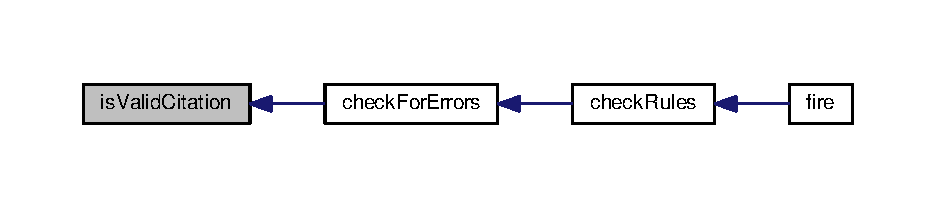
\includegraphics[width=350pt]{consistency_8js_a0cd14e63b9113fcee3fa0e999aa1ada9_icgraph}
\end{center}
\end{figure}


\index{consistency.\+js@{consistency.\+js}!match\+Rule@{match\+Rule}}
\index{match\+Rule@{match\+Rule}!consistency.\+js@{consistency.\+js}}
\subsubsection[{\texorpdfstring{match\+Rule(function\+Name, url)}{matchRule(functionName, url)}}]{\setlength{\rightskip}{0pt plus 5cm}function match\+Rule (
\begin{DoxyParamCaption}
\item[{}]{function\+Name, }
\item[{}]{url}
\end{DoxyParamCaption}
)}\hypertarget{consistency_8js_afe73f65f5154e4738551f8fe2172e4e1}{}\label{consistency_8js_afe73f65f5154e4738551f8fe2172e4e1}
match a given rule, passed by name \begin{DoxyRefDesc}{Todo}
\item[\hyperlink{todo__todo000009}{Todo}]to be written \end{DoxyRefDesc}

\begin{DoxyParams}[1]{Parameters}
string & {\em \$function\+Name} & \\
\hline
string & {\em \$url} & \\
\hline
\end{DoxyParams}
\begin{DoxyReturn}{Returns}
boolean 
\end{DoxyReturn}


Definition at line 55 of file consistency.\+js.


\hypertarget{custom_8js}{}\section{js/custom.js File Reference}
\label{custom_8js}\index{js/custom.\+js@{js/custom.\+js}}


javascript for customizing  


\subsection*{Namespaces}
\begin{DoxyCompactItemize}
\item 
 \hyperlink{namespace_bms}{Bms}
\end{DoxyCompactItemize}
\subsection*{Variables}
\begin{DoxyCompactItemize}
\item 
\hyperlink{custom_8js_ab51a99b5190515bf93a75aa0b0f3e21c}{spinner} = \textquotesingle{}$<$div class=\char`\"{}cssload-\/container\char`\"{}$>$$<$div class=\char`\"{}cssload-\/circle-\/1\char`\"{}$>$$<$div class=\char`\"{}cssload-\/circle-\/2\char`\"{}$>$$<$div class=\char`\"{}cssload-\/circle-\/3\char`\"{}$>$$<$div class=\char`\"{}cssload-\/circle-\/4\char`\"{}$>$$<$div class=\char`\"{}cssload-\/circle-\/5\char`\"{}$>$$<$div class=\char`\"{}cssload-\/circle-\/6\char`\"{}$>$$<$div class=\char`\"{}cssload-\/circle-\/7\char`\"{}$>$$<$/div$>$$<$/div$>$$<$/div$>$$<$/div$>$$<$/div$>$$<$/div$>$$<$/div$>$\textquotesingle{}
\end{DoxyCompactItemize}


\subsection{Detailed Description}
This program is free software\+: you can redistribute it and/or modify it under the terms of the G\+NU General Public License as published by the Free Software Foundation, either version 3 of the License, or (at your option) any later version.

This program is distributed in the hope that it will be useful, but W\+I\+T\+H\+O\+UT A\+NY W\+A\+R\+R\+A\+N\+TY; without even the implied warranty of M\+E\+R\+C\+H\+A\+N\+T\+A\+B\+I\+L\+I\+TY or F\+I\+T\+N\+E\+SS F\+OR A P\+A\+R\+T\+I\+C\+U\+L\+AR P\+U\+R\+P\+O\+SE. See the G\+NU General Public License for more details.

You should have received a copy of the G\+NU General Public License along with this program. If not, see \href{http://www.gnu.org/licenses/}{\tt http\+://www.\+gnu.\+org/licenses/}. 

\subsection{Variable Documentation}
\index{custom.\+js@{custom.\+js}!spinner@{spinner}}
\index{spinner@{spinner}!custom.\+js@{custom.\+js}}
\subsubsection[{\texorpdfstring{spinner}{spinner}}]{\setlength{\rightskip}{0pt plus 5cm}spinner = \textquotesingle{}$<$div class=\char`\"{}cssload-\/container\char`\"{}$>$$<$div class=\char`\"{}cssload-\/circle-\/1\char`\"{}$>$$<$div class=\char`\"{}cssload-\/circle-\/2\char`\"{}$>$$<$div class=\char`\"{}cssload-\/circle-\/3\char`\"{}$>$$<$div class=\char`\"{}cssload-\/circle-\/4\char`\"{}$>$$<$div class=\char`\"{}cssload-\/circle-\/5\char`\"{}$>$$<$div class=\char`\"{}cssload-\/circle-\/6\char`\"{}$>$$<$div class=\char`\"{}cssload-\/circle-\/7\char`\"{}$>$$<$/div$>$$<$/div$>$$<$/div$>$$<$/div$>$$<$/div$>$$<$/div$>$$<$/div$>$\textquotesingle{}}\hypertarget{custom_8js_ab51a99b5190515bf93a75aa0b0f3e21c}{}\label{custom_8js_ab51a99b5190515bf93a75aa0b0f3e21c}
spinner as a \char`\"{}worm\char`\"{} animated graphic, makes use of the css definitions in custom.\+css

string 

Definition at line 35 of file custom.\+js.


\hypertarget{dev_8js}{}\section{js/dev.js File Reference}
\label{dev_8js}\index{js/dev.\+js@{js/dev.\+js}}


javascript loadedin development mode  


\subsection*{Namespaces}
\begin{DoxyCompactItemize}
\item 
 \hyperlink{namespace_bms}{Bms}
\end{DoxyCompactItemize}
\subsection*{Variables}
\begin{DoxyCompactItemize}
\item 
\hyperlink{dev_8js_aaca7a127dea3e5f2c66c5483901969ef}{debugmode} = true
\item 
\hyperlink{dev_8js_aa9e289eddb591991c9bc7321dc5b186b}{verbose} = 3
\end{DoxyCompactItemize}


\subsection{Detailed Description}
This program is free software\+: you can redistribute it and/or modify it under the terms of the G\+NU General Public License as published by the Free Software Foundation, either version 3 of the License, or (at your option) any later version.

This program is distributed in the hope that it will be useful, but W\+I\+T\+H\+O\+UT A\+NY W\+A\+R\+R\+A\+N\+TY; without even the implied warranty of M\+E\+R\+C\+H\+A\+N\+T\+A\+B\+I\+L\+I\+TY or F\+I\+T\+N\+E\+SS F\+OR A P\+A\+R\+T\+I\+C\+U\+L\+AR P\+U\+R\+P\+O\+SE. See the G\+NU General Public License for more details.

You should have received a copy of the G\+NU General Public License along with this program. If not, see \href{http://www.gnu.org/licenses/}{\tt http\+://www.\+gnu.\+org/licenses/}. 

\subsection{Variable Documentation}
\index{dev.\+js@{dev.\+js}!debugmode@{debugmode}}
\index{debugmode@{debugmode}!dev.\+js@{dev.\+js}}
\subsubsection[{\texorpdfstring{debugmode}{debugmode}}]{\setlength{\rightskip}{0pt plus 5cm}debugmode = true}\hypertarget{dev_8js_aaca7a127dea3e5f2c66c5483901969ef}{}\label{dev_8js_aaca7a127dea3e5f2c66c5483901969ef}
in development mode\+: debugmode is set to true

Boolean 

Definition at line 32 of file dev.\+js.

\index{dev.\+js@{dev.\+js}!verbose@{verbose}}
\index{verbose@{verbose}!dev.\+js@{dev.\+js}}
\subsubsection[{\texorpdfstring{verbose}{verbose}}]{\setlength{\rightskip}{0pt plus 5cm}verbose = 3}\hypertarget{dev_8js_aa9e289eddb591991c9bc7321dc5b186b}{}\label{dev_8js_aa9e289eddb591991c9bc7321dc5b186b}
in development mode\+: verbose is set to a positive value

Number 

Definition at line 39 of file dev.\+js.


\hypertarget{frontend_8js}{}\section{js/frontend.js File Reference}
\label{frontend_8js}\index{js/frontend.\+js@{js/frontend.\+js}}


javascript functions used in the frontend  


\subsection*{Namespaces}
\begin{DoxyCompactItemize}
\item 
 \hyperlink{namespace_bms}{Bms}
\end{DoxyCompactItemize}
\subsection*{Functions}
\begin{DoxyCompactItemize}
\item 
function \hyperlink{frontend_8js_a24a888339bf25830f0d3c73e18aca77b}{show\+Date} (utime)
\item 
function \hyperlink{frontend_8js_ad1b6f7258037f83d33075afa5ed17c83}{build\+UI} (data)
\item 
function \hyperlink{frontend_8js_a21252d1127cf770a69bfa63e443fd229}{get\+Schema} (schema)
\item 
function \hyperlink{frontend_8js_a816e9b3b3cd90b9b151a46331c601fbe}{get\+Current\+Records} (id\+Provider, id\+D\+SA, schema, query\+Url, filter, nocache)
\item 
function \hyperlink{frontend_8js_a2e24b94e011170375215c3a8b745e9a4}{get\+Count\+Concept} (id\+Provider, id\+D\+SA, schema, query\+Url, concept, specifier, filter, nocache)
\item 
function \hyperlink{frontend_8js_aa6fd7ff8d2590761fcda0342978b0b22}{get\+Citation} (id\+Provider, schema, dsa, url, filter, concept, j, cached)
\item 
function \hyperlink{frontend_8js_add7d88a4ad05a1fb2478eff9a1857824}{get\+Useful\+Links} (id\+Provider, id\+D\+SA)
\item 
function \hyperlink{frontend_8js_a5f8e953a90f434851f20518b1e3baeb6}{get\+Archives} (id\+Provider, id\+D\+SA)
\item 
function \hyperlink{frontend_8js_a2f4ec7b87c92d886af91eccd0080c024}{populate\+UI} ()
\item 
function \hyperlink{frontend_8js_a026aacb2020ed839706c99a8805c244b}{show\+Progress} (id\+Provider, dsa, action, start\+Time)
\end{DoxyCompactItemize}


\subsection{Detailed Description}
This program is free software\+: you can redistribute it and/or modify it under the terms of the G\+NU General Public License as published by the Free Software Foundation, either version 3 of the License, or (at your option) any later version.

This program is distributed in the hope that it will be useful, but W\+I\+T\+H\+O\+UT A\+NY W\+A\+R\+R\+A\+N\+TY; without even the implied warranty of M\+E\+R\+C\+H\+A\+N\+T\+A\+B\+I\+L\+I\+TY or F\+I\+T\+N\+E\+SS F\+OR A P\+A\+R\+T\+I\+C\+U\+L\+AR P\+U\+R\+P\+O\+SE. See the G\+NU General Public License for more details.

You should have received a copy of the G\+NU General Public License along with this program. If not, see \href{http://www.gnu.org/licenses/}{\tt http\+://www.\+gnu.\+org/licenses/}. 

\subsection{Function Documentation}
\index{frontend.\+js@{frontend.\+js}!build\+UI@{build\+UI}}
\index{build\+UI@{build\+UI}!frontend.\+js@{frontend.\+js}}
\subsubsection[{\texorpdfstring{build\+U\+I(data)}{buildUI(data)}}]{\setlength{\rightskip}{0pt plus 5cm}function build\+UI (
\begin{DoxyParamCaption}
\item[{}]{data}
\end{DoxyParamCaption}
)}\hypertarget{frontend_8js_ad1b6f7258037f83d33075afa5ed17c83}{}\label{frontend_8js_ad1b6f7258037f83d33075afa5ed17c83}
build general User Interface


\begin{DoxyParams}[1]{Parameters}
array & {\em \$data} & The Data Provider list \\
\hline
\end{DoxyParams}
\begin{DoxyReturn}{Returns}
\{string\} 
\end{DoxyReturn}


Definition at line 54 of file frontend.\+js.



Here is the caller graph for this function\+:\nopagebreak
\begin{figure}[H]
\begin{center}
\leavevmode
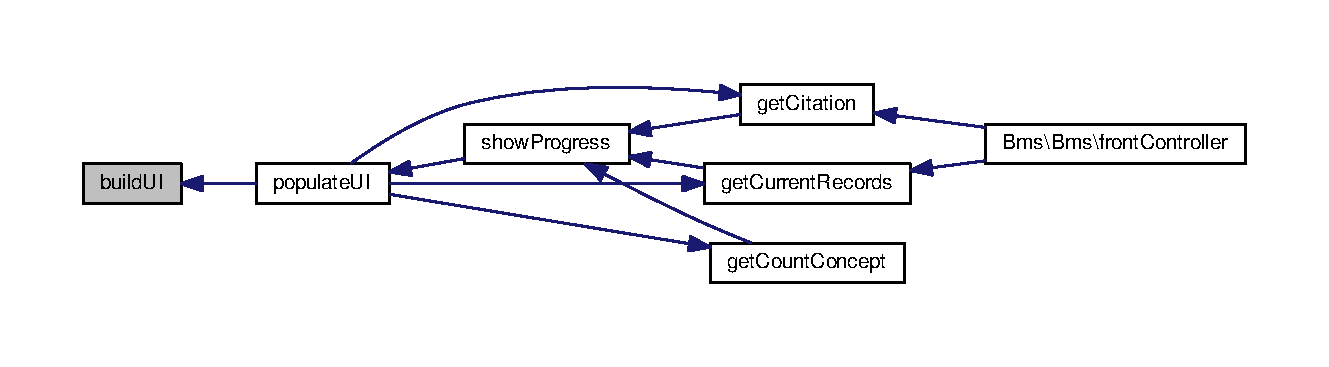
\includegraphics[width=350pt]{frontend_8js_ad1b6f7258037f83d33075afa5ed17c83_icgraph}
\end{center}
\end{figure}


\index{frontend.\+js@{frontend.\+js}!get\+Archives@{get\+Archives}}
\index{get\+Archives@{get\+Archives}!frontend.\+js@{frontend.\+js}}
\subsubsection[{\texorpdfstring{get\+Archives(id\+Provider, id\+D\+S\+A)}{getArchives(idProvider, idDSA)}}]{\setlength{\rightskip}{0pt plus 5cm}function get\+Archives (
\begin{DoxyParamCaption}
\item[{}]{id\+Provider, }
\item[{}]{id\+D\+SA}
\end{DoxyParamCaption}
)}\hypertarget{frontend_8js_a5f8e953a90f434851f20518b1e3baeb6}{}\label{frontend_8js_a5f8e953a90f434851f20518b1e3baeb6}
get xml archives of given Data Set


\begin{DoxyParams}[1]{Parameters}
int & {\em \$id\+Provider} & \\
\hline
int & {\em \$id\+D\+SA} & \\
\hline
\end{DoxyParams}
\begin{DoxyReturn}{Returns}
boolean false 
\end{DoxyReturn}


Definition at line 421 of file frontend.\+js.



Here is the caller graph for this function\+:\nopagebreak
\begin{figure}[H]
\begin{center}
\leavevmode
\includegraphics[width=350pt]{frontend_8js_a5f8e953a90f434851f20518b1e3baeb6_icgraph}
\end{center}
\end{figure}


\index{frontend.\+js@{frontend.\+js}!get\+Citation@{get\+Citation}}
\index{get\+Citation@{get\+Citation}!frontend.\+js@{frontend.\+js}}
\subsubsection[{\texorpdfstring{get\+Citation(id\+Provider, schema, dsa, url, filter, concept, j, cached)}{getCitation(idProvider, schema, dsa, url, filter, concept, j, cached)}}]{\setlength{\rightskip}{0pt plus 5cm}function get\+Citation (
\begin{DoxyParamCaption}
\item[{}]{id\+Provider, }
\item[{}]{schema, }
\item[{}]{dsa, }
\item[{}]{url, }
\item[{}]{filter, }
\item[{}]{concept, }
\item[{}]{j, }
\item[{}]{cached}
\end{DoxyParamCaption}
)}\hypertarget{frontend_8js_aa6fd7ff8d2590761fcda0342978b0b22}{}\label{frontend_8js_aa6fd7ff8d2590761fcda0342978b0b22}
get Citation Text of given Data Set


\begin{DoxyParams}[1]{Parameters}
int & {\em \$id\+Provider} & \\
\hline
string & {\em \$schema} & \\
\hline
int & {\em \$dsa} & \\
\hline
string & {\em \$url} & \\
\hline
string & {\em \$filter} & \\
\hline
string & {\em \$concept} & \\
\hline
int & {\em \$j} & index for row in UI \\
\hline
int & {\em \$cached} & 1$\vert$0 \\
\hline
\end{DoxyParams}
\begin{DoxyReturn}{Returns}
boolean false 
\end{DoxyReturn}


Definition at line 287 of file frontend.\+js.



Here is the call graph for this function\+:\nopagebreak
\begin{figure}[H]
\begin{center}
\leavevmode
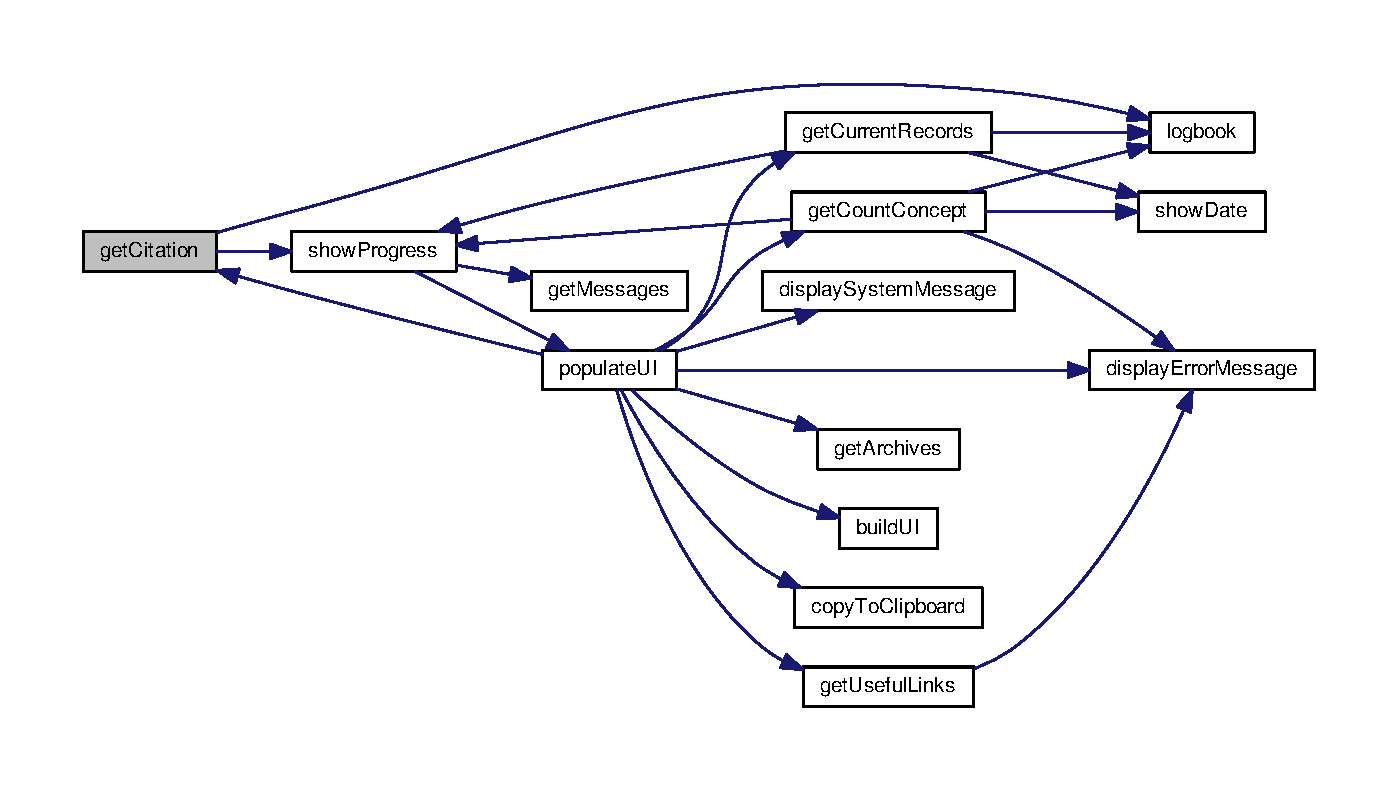
\includegraphics[width=350pt]{frontend_8js_aa6fd7ff8d2590761fcda0342978b0b22_cgraph}
\end{center}
\end{figure}




Here is the caller graph for this function\+:\nopagebreak
\begin{figure}[H]
\begin{center}
\leavevmode
\includegraphics[width=350pt]{frontend_8js_aa6fd7ff8d2590761fcda0342978b0b22_icgraph}
\end{center}
\end{figure}


\index{frontend.\+js@{frontend.\+js}!get\+Count\+Concept@{get\+Count\+Concept}}
\index{get\+Count\+Concept@{get\+Count\+Concept}!frontend.\+js@{frontend.\+js}}
\subsubsection[{\texorpdfstring{get\+Count\+Concept(id\+Provider, id\+D\+S\+A, schema, query\+Url, concept, specifier, filter, nocache)}{getCountConcept(idProvider, idDSA, schema, queryUrl, concept, specifier, filter, nocache)}}]{\setlength{\rightskip}{0pt plus 5cm}function get\+Count\+Concept (
\begin{DoxyParamCaption}
\item[{}]{id\+Provider, }
\item[{}]{id\+D\+SA, }
\item[{}]{schema, }
\item[{}]{query\+Url, }
\item[{}]{concept, }
\item[{}]{specifier, }
\item[{}]{filter, }
\item[{}]{nocache}
\end{DoxyParamCaption}
)}\hypertarget{frontend_8js_a2e24b94e011170375215c3a8b745e9a4}{}\label{frontend_8js_a2e24b94e011170375215c3a8b745e9a4}
count the occurrences of a given concept


\begin{DoxyParams}[1]{Parameters}
int & {\em \$id\+Provider} & \\
\hline
int & {\em \$id\+D\+SA} & \\
\hline
string & {\em \$schema} & \\
\hline
string & {\em \$query\+Url} & \\
\hline
string & {\em \$concept} & a capability, like /\+Data\+Sets/\+Data\+Set/\+Units/\+Unit/\+Unit\+ID \\
\hline
int & {\em \$specifier} & a bitmap of T\+O\+T\+AL, D\+I\+S\+T\+I\+N\+CT, D\+R\+O\+P\+P\+ED \\
\hline
string & {\em \$filter} & complex filter\+: $<$like$>$....$<$/like$>$ \\
\hline
int & {\em \$nocache} & 1$\vert$0 \\
\hline
\end{DoxyParams}
\begin{DoxyReturn}{Returns}
boolean false 
\end{DoxyReturn}


Definition at line 202 of file frontend.\+js.



Here is the call graph for this function\+:\nopagebreak
\begin{figure}[H]
\begin{center}
\leavevmode
\includegraphics[width=350pt]{frontend_8js_a2e24b94e011170375215c3a8b745e9a4_cgraph}
\end{center}
\end{figure}




Here is the caller graph for this function\+:\nopagebreak
\begin{figure}[H]
\begin{center}
\leavevmode
\includegraphics[width=350pt]{frontend_8js_a2e24b94e011170375215c3a8b745e9a4_icgraph}
\end{center}
\end{figure}


\index{frontend.\+js@{frontend.\+js}!get\+Current\+Records@{get\+Current\+Records}}
\index{get\+Current\+Records@{get\+Current\+Records}!frontend.\+js@{frontend.\+js}}
\subsubsection[{\texorpdfstring{get\+Current\+Records(id\+Provider, id\+D\+S\+A, schema, query\+Url, filter, nocache)}{getCurrentRecords(idProvider, idDSA, schema, queryUrl, filter, nocache)}}]{\setlength{\rightskip}{0pt plus 5cm}function get\+Current\+Records (
\begin{DoxyParamCaption}
\item[{}]{id\+Provider, }
\item[{}]{id\+D\+SA, }
\item[{}]{schema, }
\item[{}]{query\+Url, }
\item[{}]{filter, }
\item[{}]{nocache}
\end{DoxyParamCaption}
)}\hypertarget{frontend_8js_a816e9b3b3cd90b9b151a46331c601fbe}{}\label{frontend_8js_a816e9b3b3cd90b9b151a46331c601fbe}
get Number of Current Records


\begin{DoxyParams}[1]{Parameters}
int & {\em \$id\+Provider} & \\
\hline
int & {\em \$id\+D\+SA} & \\
\hline
string & {\em \$schema} & \\
\hline
string & {\em \$query\+Url} & \\
\hline
string & {\em \$filter} & complex filter $<$like$>$...$<$/like$>$ \\
\hline
int & {\em \$nocache} & 0 or 1 \\
\hline
\end{DoxyParams}
\begin{DoxyReturn}{Returns}
boolean false 
\end{DoxyReturn}


Definition at line 119 of file frontend.\+js.



Here is the call graph for this function\+:\nopagebreak
\begin{figure}[H]
\begin{center}
\leavevmode
\includegraphics[width=350pt]{frontend_8js_a816e9b3b3cd90b9b151a46331c601fbe_cgraph}
\end{center}
\end{figure}




Here is the caller graph for this function\+:\nopagebreak
\begin{figure}[H]
\begin{center}
\leavevmode
\includegraphics[width=350pt]{frontend_8js_a816e9b3b3cd90b9b151a46331c601fbe_icgraph}
\end{center}
\end{figure}


\index{frontend.\+js@{frontend.\+js}!get\+Schema@{get\+Schema}}
\index{get\+Schema@{get\+Schema}!frontend.\+js@{frontend.\+js}}
\subsubsection[{\texorpdfstring{get\+Schema(schema)}{getSchema(schema)}}]{\setlength{\rightskip}{0pt plus 5cm}function get\+Schema (
\begin{DoxyParamCaption}
\item[{}]{schema}
\end{DoxyParamCaption}
)}\hypertarget{frontend_8js_a21252d1127cf770a69bfa63e443fd229}{}\label{frontend_8js_a21252d1127cf770a69bfa63e443fd229}
get Schema shortname


\begin{DoxyParams}[1]{Parameters}
string & {\em \$schema} & \\
\hline
\end{DoxyParams}
\begin{DoxyReturn}{Returns}
string 
\end{DoxyReturn}


Definition at line 86 of file frontend.\+js.



Here is the caller graph for this function\+:\nopagebreak
\begin{figure}[H]
\begin{center}
\leavevmode
\includegraphics[width=307pt]{frontend_8js_a21252d1127cf770a69bfa63e443fd229_icgraph}
\end{center}
\end{figure}


\index{frontend.\+js@{frontend.\+js}!get\+Useful\+Links@{get\+Useful\+Links}}
\index{get\+Useful\+Links@{get\+Useful\+Links}!frontend.\+js@{frontend.\+js}}
\subsubsection[{\texorpdfstring{get\+Useful\+Links(id\+Provider, id\+D\+S\+A)}{getUsefulLinks(idProvider, idDSA)}}]{\setlength{\rightskip}{0pt plus 5cm}function get\+Useful\+Links (
\begin{DoxyParamCaption}
\item[{}]{id\+Provider, }
\item[{}]{id\+D\+SA}
\end{DoxyParamCaption}
)}\hypertarget{frontend_8js_add7d88a4ad05a1fb2478eff9a1857824}{}\label{frontend_8js_add7d88a4ad05a1fb2478eff9a1857824}
get useful Links of given Data Set


\begin{DoxyParams}[1]{Parameters}
int & {\em \$id\+Provider} & \\
\hline
int & {\em \$id\+D\+SA} & \\
\hline
\end{DoxyParams}
\begin{DoxyReturn}{Returns}
boolean false 
\end{DoxyReturn}


Definition at line 353 of file frontend.\+js.



Here is the call graph for this function\+:\nopagebreak
\begin{figure}[H]
\begin{center}
\leavevmode
\includegraphics[width=306pt]{frontend_8js_add7d88a4ad05a1fb2478eff9a1857824_cgraph}
\end{center}
\end{figure}




Here is the caller graph for this function\+:\nopagebreak
\begin{figure}[H]
\begin{center}
\leavevmode
\includegraphics[width=350pt]{frontend_8js_add7d88a4ad05a1fb2478eff9a1857824_icgraph}
\end{center}
\end{figure}


\index{frontend.\+js@{frontend.\+js}!populate\+UI@{populate\+UI}}
\index{populate\+UI@{populate\+UI}!frontend.\+js@{frontend.\+js}}
\subsubsection[{\texorpdfstring{populate\+U\+I()}{populateUI()}}]{\setlength{\rightskip}{0pt plus 5cm}function populate\+UI (
\begin{DoxyParamCaption}
{}
\end{DoxyParamCaption}
)}\hypertarget{frontend_8js_a2f4ec7b87c92d886af91eccd0080c024}{}\label{frontend_8js_a2f4ec7b87c92d886af91eccd0080c024}
Main function\+: populates the UI

\begin{DoxyReturn}{Returns}
boolean false 
\end{DoxyReturn}


Definition at line 482 of file frontend.\+js.



Here is the call graph for this function\+:\nopagebreak
\begin{figure}[H]
\begin{center}
\leavevmode
\includegraphics[width=350pt]{frontend_8js_a2f4ec7b87c92d886af91eccd0080c024_cgraph}
\end{center}
\end{figure}




Here is the caller graph for this function\+:\nopagebreak
\begin{figure}[H]
\begin{center}
\leavevmode
\includegraphics[width=350pt]{frontend_8js_a2f4ec7b87c92d886af91eccd0080c024_icgraph}
\end{center}
\end{figure}


\index{frontend.\+js@{frontend.\+js}!show\+Date@{show\+Date}}
\index{show\+Date@{show\+Date}!frontend.\+js@{frontend.\+js}}
\subsubsection[{\texorpdfstring{show\+Date(utime)}{showDate(utime)}}]{\setlength{\rightskip}{0pt plus 5cm}function show\+Date (
\begin{DoxyParamCaption}
\item[{}]{utime}
\end{DoxyParamCaption}
)}\hypertarget{frontend_8js_a24a888339bf25830f0d3c73e18aca77b}{}\label{frontend_8js_a24a888339bf25830f0d3c73e18aca77b}
display a date-\/time string


\begin{DoxyParams}[1]{Parameters}
int & {\em \$utime} & \\
\hline
\end{DoxyParams}
\begin{DoxyReturn}{Returns}
string 
\end{DoxyReturn}


Definition at line 40 of file frontend.\+js.



Here is the caller graph for this function\+:\nopagebreak
\begin{figure}[H]
\begin{center}
\leavevmode
\includegraphics[width=350pt]{frontend_8js_a24a888339bf25830f0d3c73e18aca77b_icgraph}
\end{center}
\end{figure}


\index{frontend.\+js@{frontend.\+js}!show\+Progress@{show\+Progress}}
\index{show\+Progress@{show\+Progress}!frontend.\+js@{frontend.\+js}}
\subsubsection[{\texorpdfstring{show\+Progress(id\+Provider, dsa, action, start\+Time)}{showProgress(idProvider, dsa, action, startTime)}}]{\setlength{\rightskip}{0pt plus 5cm}function show\+Progress (
\begin{DoxyParamCaption}
\item[{}]{id\+Provider, }
\item[{}]{dsa, }
\item[{}]{action, }
\item[{}]{start\+Time}
\end{DoxyParamCaption}
)}\hypertarget{frontend_8js_a026aacb2020ed839706c99a8805c244b}{}\label{frontend_8js_a026aacb2020ed839706c99a8805c244b}
shows waiting time for http requests to B\+PS


\begin{DoxyParams}[1]{Parameters}
int & {\em \$id\+Provider} & \\
\hline
string & {\em \$dsa} & \\
\hline
string & {\em \$action} & \\
\hline
float & {\em \$start\+Time} & \\
\hline
\end{DoxyParams}
\begin{DoxyReturn}{Returns}
boolean false 
\end{DoxyReturn}


Definition at line 773 of file frontend.\+js.



Here is the call graph for this function\+:\nopagebreak
\begin{figure}[H]
\begin{center}
\leavevmode
\includegraphics[width=350pt]{frontend_8js_a026aacb2020ed839706c99a8805c244b_cgraph}
\end{center}
\end{figure}




Here is the caller graph for this function\+:\nopagebreak
\begin{figure}[H]
\begin{center}
\leavevmode
\includegraphics[width=350pt]{frontend_8js_a026aacb2020ed839706c99a8805c244b_icgraph}
\end{center}
\end{figure}



\hypertarget{general_8js}{}\section{js/general.js File Reference}
\label{general_8js}\index{js/general.\+js@{js/general.\+js}}


javascript general settings functions  


\subsection*{Namespaces}
\begin{DoxyCompactItemize}
\item 
 \hyperlink{namespace_bms}{Bms}
\end{DoxyCompactItemize}
\subsection*{Functions}
\begin{DoxyCompactItemize}
\item 
function \hyperlink{general_8js_ad9f2873ff9e09926e2f18c529721c6f8}{get\+Messages} (path)
\item 
function \hyperlink{general_8js_aecfeb655371b751d36422b7a93a66279}{display\+System\+Message} (msg, alert, duration)
\item 
function \hyperlink{general_8js_aae7d603c7aa8402259bc3e7bb47ead5c}{hide\+System\+Message} ()
\item 
function \hyperlink{general_8js_a3c52670d7ece95bdca65208692bc18f2}{display\+Error\+Message} (elt, msg, mode)
\item 
function \hyperlink{general_8js_ae9d354184ac1776e35e40dc85568f6ed}{show\+Concurrent\+Requests} ()
\item 
function \hyperlink{general_8js_a33e21da30cef3db82208e64a6801aa44}{logbook} (id\+Provider, schema, dsa, concept, action, time\+Elapsed)
\item 
function \hyperlink{general_8js_ab624ce9aebffbb8bc3159502c4afc32b}{copy\+To\+Clipboard} (elem)
\item 
function \hyperlink{general_8js_a0edb409ffb3ee2517792cf9068954410}{format\+Xml} (xml)
\end{DoxyCompactItemize}
\subsection*{Variables}
\begin{DoxyCompactItemize}
\item 
\hyperlink{general_8js_af460b1b8a09a5b3b38739122de4b934e}{biocase\+Response\+Url} = \char`\"{}/pywrapper.\+cgi?dsa=\char`\"{}
\item 
\hyperlink{general_8js_a7b0ba1f3880fe6b39f5cdc1e1307c56d}{biocase\+Query\+Url} = \char`\"{}utilities/queryforms/qf\+\_\+manual.\+cgi?dsa=\char`\"{}
\item 
\hyperlink{general_8js_a17dea9711da86f7ede3d3090df67dfda}{biocase\+Local\+Query\+Tool\+Url} = \char`\"{}querytool/main.\+cgi?dsa=\char`\"{}
\item 
\hyperlink{general_8js_ab8140947611504abcb64a4c277effcf5}{message} = \{\}
\item 
\hyperlink{general_8js_aaca7a127dea3e5f2c66c5483901969ef}{debugmode} = false
\item 
\hyperlink{general_8js_aa9e289eddb591991c9bc7321dc5b186b}{verbose} = 0
\item 
\hyperlink{general_8js_ab51a99b5190515bf93a75aa0b0f3e21c}{spinner} = \char`\"{}$<$span class=\textquotesingle{}glyphicon glyphicon-\/refresh gly-\/spin\textquotesingle{}/$>$\char`\"{}
\item 
\hyperlink{general_8js_a95f4dd4429a1cdb9f09ce3444d78ed56}{nb\+Ajax\+Calls} = 0
\end{DoxyCompactItemize}


\subsection{Detailed Description}
This program is free software\+: you can redistribute it and/or modify it under the terms of the G\+NU General Public License as published by the Free Software Foundation, either version 3 of the License, or (at your option) any later version.

This program is distributed in the hope that it will be useful, but W\+I\+T\+H\+O\+UT A\+NY W\+A\+R\+R\+A\+N\+TY; without even the implied warranty of M\+E\+R\+C\+H\+A\+N\+T\+A\+B\+I\+L\+I\+TY or F\+I\+T\+N\+E\+SS F\+OR A P\+A\+R\+T\+I\+C\+U\+L\+AR P\+U\+R\+P\+O\+SE. See the G\+NU General Public License for more details.

You should have received a copy of the G\+NU General Public License along with this program. If not, see \href{http://www.gnu.org/licenses/}{\tt http\+://www.\+gnu.\+org/licenses/}. 

\subsection{Function Documentation}
\index{general.\+js@{general.\+js}!copy\+To\+Clipboard@{copy\+To\+Clipboard}}
\index{copy\+To\+Clipboard@{copy\+To\+Clipboard}!general.\+js@{general.\+js}}
\subsubsection[{\texorpdfstring{copy\+To\+Clipboard(elem)}{copyToClipboard(elem)}}]{\setlength{\rightskip}{0pt plus 5cm}function copy\+To\+Clipboard (
\begin{DoxyParamCaption}
\item[{}]{elem}
\end{DoxyParamCaption}
)}\hypertarget{general_8js_ab624ce9aebffbb8bc3159502c4afc32b}{}\label{general_8js_ab624ce9aebffbb8bc3159502c4afc32b}
copy selected text portion to Clipboard


\begin{DoxyParams}[1]{Parameters}
object & {\em \$elem} & j\+Query object \\
\hline
\end{DoxyParams}
\begin{DoxyReturn}{Returns}
bool 
\end{DoxyReturn}


Definition at line 224 of file general.\+js.



Here is the caller graph for this function\+:\nopagebreak
\begin{figure}[H]
\begin{center}
\leavevmode
\includegraphics[width=350pt]{general_8js_ab624ce9aebffbb8bc3159502c4afc32b_icgraph}
\end{center}
\end{figure}


\index{general.\+js@{general.\+js}!display\+Error\+Message@{display\+Error\+Message}}
\index{display\+Error\+Message@{display\+Error\+Message}!general.\+js@{general.\+js}}
\subsubsection[{\texorpdfstring{display\+Error\+Message(elt, msg, mode)}{displayErrorMessage(elt, msg, mode)}}]{\setlength{\rightskip}{0pt plus 5cm}function display\+Error\+Message (
\begin{DoxyParamCaption}
\item[{}]{elt, }
\item[{}]{msg, }
\item[{}]{mode}
\end{DoxyParamCaption}
)}\hypertarget{general_8js_a3c52670d7ece95bdca65208692bc18f2}{}\label{general_8js_a3c52670d7ece95bdca65208692bc18f2}
displays a system error message as an answer of an operation


\begin{DoxyParams}[1]{Parameters}
string & {\em \$elt} & the j\+Query Element where the message is displayed \\
\hline
string & {\em \$msg} & the message text \\
\hline
string & {\em \$mode} & replace or add at end of the j\+Query element elt \\
\hline
\end{DoxyParams}
\begin{DoxyReturn}{Returns}
void 
\end{DoxyReturn}


Definition at line 144 of file general.\+js.



Here is the caller graph for this function\+:\nopagebreak
\begin{figure}[H]
\begin{center}
\leavevmode
\includegraphics[width=350pt]{general_8js_a3c52670d7ece95bdca65208692bc18f2_icgraph}
\end{center}
\end{figure}


\index{general.\+js@{general.\+js}!display\+System\+Message@{display\+System\+Message}}
\index{display\+System\+Message@{display\+System\+Message}!general.\+js@{general.\+js}}
\subsubsection[{\texorpdfstring{display\+System\+Message(msg, alert, duration)}{displaySystemMessage(msg, alert, duration)}}]{\setlength{\rightskip}{0pt plus 5cm}function display\+System\+Message (
\begin{DoxyParamCaption}
\item[{}]{msg, }
\item[{}]{alert, }
\item[{}]{duration}
\end{DoxyParamCaption}
)}\hypertarget{general_8js_aecfeb655371b751d36422b7a93a66279}{}\label{general_8js_aecfeb655371b751d36422b7a93a66279}
displays a system message as an answer of an operation


\begin{DoxyParams}[1]{Parameters}
string & {\em \$msg} & the message text \\
\hline
string & {\em \$alert} & info,warning,success,danger \\
\hline
int & {\em \$duration} & \\
\hline
\end{DoxyParams}
\begin{DoxyReturn}{Returns}
void 
\end{DoxyReturn}


Definition at line 114 of file general.\+js.



Here is the caller graph for this function\+:\nopagebreak
\begin{figure}[H]
\begin{center}
\leavevmode
\includegraphics[width=350pt]{general_8js_aecfeb655371b751d36422b7a93a66279_icgraph}
\end{center}
\end{figure}


\index{general.\+js@{general.\+js}!format\+Xml@{format\+Xml}}
\index{format\+Xml@{format\+Xml}!general.\+js@{general.\+js}}
\subsubsection[{\texorpdfstring{format\+Xml(xml)}{formatXml(xml)}}]{\setlength{\rightskip}{0pt plus 5cm}function format\+Xml (
\begin{DoxyParamCaption}
\item[{}]{xml}
\end{DoxyParamCaption}
)}\hypertarget{general_8js_a0edb409ffb3ee2517792cf9068954410}{}\label{general_8js_a0edb409ffb3ee2517792cf9068954410}
pretty prints a X\+ML string


\begin{DoxyParams}[1]{Parameters}
string & {\em \$xml} & a raw X\+ML string \\
\hline
\end{DoxyParams}
\begin{DoxyReturn}{Returns}
\{String\} 
\end{DoxyReturn}


Definition at line 264 of file general.\+js.

\index{general.\+js@{general.\+js}!get\+Messages@{get\+Messages}}
\index{get\+Messages@{get\+Messages}!general.\+js@{general.\+js}}
\subsubsection[{\texorpdfstring{get\+Messages(path)}{getMessages(path)}}]{\setlength{\rightskip}{0pt plus 5cm}function get\+Messages (
\begin{DoxyParamCaption}
\item[{}]{path}
\end{DoxyParamCaption}
)}\hypertarget{general_8js_ad9f2873ff9e09926e2f18c529721c6f8}{}\label{general_8js_ad9f2873ff9e09926e2f18c529721c6f8}
loads system messages into global variable \char`\"{}message\char`\"{}


\begin{DoxyParams}[1]{Parameters}
string & {\em \$path} & \\
\hline
\end{DoxyParams}
\begin{DoxyReturn}{Returns}
boolean false 
\end{DoxyReturn}


Definition at line 85 of file general.\+js.



Here is the caller graph for this function\+:\nopagebreak
\begin{figure}[H]
\begin{center}
\leavevmode
\includegraphics[width=350pt]{general_8js_ad9f2873ff9e09926e2f18c529721c6f8_icgraph}
\end{center}
\end{figure}


\index{general.\+js@{general.\+js}!hide\+System\+Message@{hide\+System\+Message}}
\index{hide\+System\+Message@{hide\+System\+Message}!general.\+js@{general.\+js}}
\subsubsection[{\texorpdfstring{hide\+System\+Message()}{hideSystemMessage()}}]{\setlength{\rightskip}{0pt plus 5cm}function hide\+System\+Message (
\begin{DoxyParamCaption}
{}
\end{DoxyParamCaption}
)}\hypertarget{general_8js_aae7d603c7aa8402259bc3e7bb47ead5c}{}\label{general_8js_aae7d603c7aa8402259bc3e7bb47ead5c}
hides a system message

\begin{DoxyReturn}{Returns}
void 
\end{DoxyReturn}


Definition at line 132 of file general.\+js.

\index{general.\+js@{general.\+js}!logbook@{logbook}}
\index{logbook@{logbook}!general.\+js@{general.\+js}}
\subsubsection[{\texorpdfstring{logbook(id\+Provider, schema, dsa, concept, action, time\+Elapsed)}{logbook(idProvider, schema, dsa, concept, action, timeElapsed)}}]{\setlength{\rightskip}{0pt plus 5cm}function logbook (
\begin{DoxyParamCaption}
\item[{}]{id\+Provider, }
\item[{}]{schema, }
\item[{}]{dsa, }
\item[{}]{concept, }
\item[{}]{action, }
\item[{}]{time\+Elapsed}
\end{DoxyParamCaption}
)}\hypertarget{general_8js_a33e21da30cef3db82208e64a6801aa44}{}\label{general_8js_a33e21da30cef3db82208e64a6801aa44}
writes selected infos to logbook


\begin{DoxyParams}[1]{Parameters}
int & {\em \$id\+Provider} & \\
\hline
string & {\em \$schema} & \\
\hline
int & {\em \$dsa} & \\
\hline
string & {\em \$concept} & \\
\hline
string & {\em \$action} & \\
\hline
float & {\em \$time\+Elapsed} & \\
\hline
\end{DoxyParams}
\begin{DoxyReturn}{Returns}
boolean false 
\end{DoxyReturn}


Definition at line 201 of file general.\+js.



Here is the caller graph for this function\+:\nopagebreak
\begin{figure}[H]
\begin{center}
\leavevmode
\includegraphics[width=350pt]{general_8js_a33e21da30cef3db82208e64a6801aa44_icgraph}
\end{center}
\end{figure}


\index{general.\+js@{general.\+js}!show\+Concurrent\+Requests@{show\+Concurrent\+Requests}}
\index{show\+Concurrent\+Requests@{show\+Concurrent\+Requests}!general.\+js@{general.\+js}}
\subsubsection[{\texorpdfstring{show\+Concurrent\+Requests()}{showConcurrentRequests()}}]{\setlength{\rightskip}{0pt plus 5cm}function show\+Concurrent\+Requests (
\begin{DoxyParamCaption}
{}
\end{DoxyParamCaption}
)}\hypertarget{general_8js_ae9d354184ac1776e35e40dc85568f6ed}{}\label{general_8js_ae9d354184ac1776e35e40dc85568f6ed}
shows number of concurrent requests

\begin{DoxyReturn}{Returns}
void 
\end{DoxyReturn}


Definition at line 159 of file general.\+js.



\subsection{Variable Documentation}
\index{general.\+js@{general.\+js}!biocase\+Local\+Query\+Tool\+Url@{biocase\+Local\+Query\+Tool\+Url}}
\index{biocase\+Local\+Query\+Tool\+Url@{biocase\+Local\+Query\+Tool\+Url}!general.\+js@{general.\+js}}
\subsubsection[{\texorpdfstring{biocase\+Local\+Query\+Tool\+Url}{biocaseLocalQueryToolUrl}}]{\setlength{\rightskip}{0pt plus 5cm}biocase\+Local\+Query\+Tool\+Url = \char`\"{}querytool/main.\+cgi?dsa=\char`\"{}}\hypertarget{general_8js_a17dea9711da86f7ede3d3090df67dfda}{}\label{general_8js_a17dea9711da86f7ede3d3090df67dfda}
defines the biocase software endpoint Local Query G\+UI 

Definition at line 46 of file general.\+js.

\index{general.\+js@{general.\+js}!biocase\+Query\+Url@{biocase\+Query\+Url}}
\index{biocase\+Query\+Url@{biocase\+Query\+Url}!general.\+js@{general.\+js}}
\subsubsection[{\texorpdfstring{biocase\+Query\+Url}{biocaseQueryUrl}}]{\setlength{\rightskip}{0pt plus 5cm}biocase\+Query\+Url = \char`\"{}utilities/queryforms/qf\+\_\+manual.\+cgi?dsa=\char`\"{}}\hypertarget{general_8js_a7b0ba1f3880fe6b39f5cdc1e1307c56d}{}\label{general_8js_a7b0ba1f3880fe6b39f5cdc1e1307c56d}
defines the biocase software endpoint G\+UI 

Definition at line 40 of file general.\+js.

\index{general.\+js@{general.\+js}!biocase\+Response\+Url@{biocase\+Response\+Url}}
\index{biocase\+Response\+Url@{biocase\+Response\+Url}!general.\+js@{general.\+js}}
\subsubsection[{\texorpdfstring{biocase\+Response\+Url}{biocaseResponseUrl}}]{\setlength{\rightskip}{0pt plus 5cm}biocase\+Response\+Url = \char`\"{}/pywrapper.\+cgi?dsa=\char`\"{}}\hypertarget{general_8js_af460b1b8a09a5b3b38739122de4b934e}{}\label{general_8js_af460b1b8a09a5b3b38739122de4b934e}
defines the biocase software U\+RL response for a given data source 

Definition at line 34 of file general.\+js.

\index{general.\+js@{general.\+js}!debugmode@{debugmode}}
\index{debugmode@{debugmode}!general.\+js@{general.\+js}}
\subsubsection[{\texorpdfstring{debugmode}{debugmode}}]{\setlength{\rightskip}{0pt plus 5cm}debugmode = false}\hypertarget{general_8js_aaca7a127dea3e5f2c66c5483901969ef}{}\label{general_8js_aaca7a127dea3e5f2c66c5483901969ef}
may be overwritten by scripts or G\+E\+T-\/parameters 

Definition at line 58 of file general.\+js.

\index{general.\+js@{general.\+js}!message@{message}}
\index{message@{message}!general.\+js@{general.\+js}}
\subsubsection[{\texorpdfstring{message}{message}}]{\setlength{\rightskip}{0pt plus 5cm}message = \{\}}\hypertarget{general_8js_ab8140947611504abcb64a4c277effcf5}{}\label{general_8js_ab8140947611504abcb64a4c277effcf5}
defines the system messages 

Definition at line 52 of file general.\+js.

\index{general.\+js@{general.\+js}!nb\+Ajax\+Calls@{nb\+Ajax\+Calls}}
\index{nb\+Ajax\+Calls@{nb\+Ajax\+Calls}!general.\+js@{general.\+js}}
\subsubsection[{\texorpdfstring{nb\+Ajax\+Calls}{nbAjaxCalls}}]{\setlength{\rightskip}{0pt plus 5cm}nb\+Ajax\+Calls = 0}\hypertarget{general_8js_a95f4dd4429a1cdb9f09ce3444d78ed56}{}\label{general_8js_a95f4dd4429a1cdb9f09ce3444d78ed56}
number of pending calls to the B\+PS is overwritten dynamically 

Definition at line 77 of file general.\+js.

\index{general.\+js@{general.\+js}!spinner@{spinner}}
\index{spinner@{spinner}!general.\+js@{general.\+js}}
\subsubsection[{\texorpdfstring{spinner}{spinner}}]{\setlength{\rightskip}{0pt plus 5cm}spinner = \char`\"{}$<$span class=\textquotesingle{}glyphicon glyphicon-\/refresh gly-\/spin\textquotesingle{}/$>$\char`\"{}}\hypertarget{general_8js_ab51a99b5190515bf93a75aa0b0f3e21c}{}\label{general_8js_ab51a99b5190515bf93a75aa0b0f3e21c}
may be overwritten by \hyperlink{custom_8js}{js/custom.\+js} 

Definition at line 70 of file general.\+js.

\index{general.\+js@{general.\+js}!verbose@{verbose}}
\index{verbose@{verbose}!general.\+js@{general.\+js}}
\subsubsection[{\texorpdfstring{verbose}{verbose}}]{\setlength{\rightskip}{0pt plus 5cm}verbose = 0}\hypertarget{general_8js_aa9e289eddb591991c9bc7321dc5b186b}{}\label{general_8js_aa9e289eddb591991c9bc7321dc5b186b}
may be overwritten by scripts or G\+E\+T-\/parameters 

Definition at line 64 of file general.\+js.


\hypertarget{landingpage_8js}{}\section{js/landingpage.js File Reference}
\label{landingpage_8js}\index{js/landingpage.\+js@{js/landingpage.\+js}}


javascript statements for the landingpage  


\subsection*{Namespaces}
\begin{DoxyCompactItemize}
\item 
 \hyperlink{namespace_bms}{Bms}
\end{DoxyCompactItemize}


\subsection{Detailed Description}
This program is free software\+: you can redistribute it and/or modify it under the terms of the G\+NU General Public License as published by the Free Software Foundation, either version 3 of the License, or (at your option) any later version.

This program is distributed in the hope that it will be useful, but W\+I\+T\+H\+O\+UT A\+NY W\+A\+R\+R\+A\+N\+TY; without even the implied warranty of M\+E\+R\+C\+H\+A\+N\+T\+A\+B\+I\+L\+I\+TY or F\+I\+T\+N\+E\+SS F\+OR A P\+A\+R\+T\+I\+C\+U\+L\+AR P\+U\+R\+P\+O\+SE. See the G\+NU General Public License for more details.

You should have received a copy of the G\+NU General Public License along with this program. If not, see \href{http://www.gnu.org/licenses/}{\tt http\+://www.\+gnu.\+org/licenses/}. 
\hypertarget{landingpage_8php}{}\section{landingpage.\+php File Reference}
\label{landingpage_8php}\index{landingpage.\+php@{landingpage.\+php}}


landing page for A\+B\+C\+D2.\+06 raw xml  


\subsection*{Namespaces}
\begin{DoxyCompactItemize}
\item 
 \hyperlink{namespace_bms}{Bms}
\end{DoxyCompactItemize}


\subsection{Detailed Description}
Bio\+C\+A\+Se Monitor 2.\+1 \begin{DoxyCopyright}{Copyright}
(C) 2013-\/2018 www.\+museumfuernaturkunde.\+berlin 
\end{DoxyCopyright}
\begin{DoxyAuthor}{Author}
\href{mailto:thomas.pfuhl@mfn.berlin}{\tt thomas.\+pfuhl@mfn.\+berlin} based on Version 1.\+4 written by \href{mailto:falko.gloeckler@mfn.berlin}{\tt falko.\+gloeckler@mfn.\+berlin}
\end{DoxyAuthor}
This program is free software\+: you can redistribute it and/or modify it under the terms of the G\+NU General Public License as published by the Free Software Foundation, either version 3 of the License, or (at your option) any later version.

This program is distributed in the hope that it will be useful, but W\+I\+T\+H\+O\+UT A\+NY W\+A\+R\+R\+A\+N\+TY; without even the implied warranty of M\+E\+R\+C\+H\+A\+N\+T\+A\+B\+I\+L\+I\+TY or F\+I\+T\+N\+E\+SS F\+OR A P\+A\+R\+T\+I\+C\+U\+L\+AR P\+U\+R\+P\+O\+SE. See the G\+NU General Public License for more details.

You should have received a copy of the G\+NU General Public License along with this program. If not, see \href{http://www.gnu.org/licenses/}{\tt http\+://www.\+gnu.\+org/licenses/}. 
\hypertarget{logbook_8php}{}\section{logbook.\+php File Reference}
\label{logbook_8php}\index{logbook.\+php@{logbook.\+php}}


statistics to log resquests to the B\+PS installations  


\subsection*{Namespaces}
\begin{DoxyCompactItemize}
\item 
 \hyperlink{namespace_consistency}{Consistency}
\item 
 \hyperlink{namespace_bms}{Bms}
\end{DoxyCompactItemize}


\subsection{Detailed Description}
This program is free software\+: you can redistribute it and/or modify it under the terms of the G\+NU General Public License as published by the Free Software Foundation, either version 3 of the License, or (at your option) any later version.

This program is distributed in the hope that it will be useful, but W\+I\+T\+H\+O\+UT A\+NY W\+A\+R\+R\+A\+N\+TY; without even the implied warranty of M\+E\+R\+C\+H\+A\+N\+T\+A\+B\+I\+L\+I\+TY or F\+I\+T\+N\+E\+SS F\+OR A P\+A\+R\+T\+I\+C\+U\+L\+AR P\+U\+R\+P\+O\+SE. See the G\+NU General Public License for more details.

You should have received a copy of the G\+NU General Public License along with this program. If not, see \href{http://www.gnu.org/licenses/}{\tt http\+://www.\+gnu.\+org/licenses/}. 
%--- End generated contents ---

% Index
\backmatter
\newpage
\phantomsection
\clearemptydoublepage
\addcontentsline{toc}{chapter}{Index}
\printindex

\end{document}
